% SIAM Article Template
\documentclass[review,onefignum,onetabnum]{article}
%\documentclass[article,onefignum,onetabnum]{siamonline220329} %review %article %siamonline220329

% \usepackage{a4wide}

\usepackage{amsmath,amssymb,bbm,amsthm}
\usepackage{dsfont}
\usepackage{graphicx,framed}
\usepackage{url,bm}
\usepackage{color}
\usepackage{float}
%\usepackage{algorithm}
\RequirePackage{algorithm}[0.1]
% \renewcommand{\ALG@name}{Algorithm}
\usepackage{algpseudocode} % ce package crée un petit beug de mise en page en première page
%\usepackage{algorithm2e}
%\usepackage{algorithmic}
\usepackage{subfigure}
\usepackage{epstopdf,framed}
\usepackage{mathrsfs,multirow}
\usepackage{cite}
%\usepackage[color,draft,notref]{showkeys}
\usepackage{comment}
\usepackage{xspace}
\usepackage[colorlinks=True]{hyperref}

\usepackage{xcolor}
\hypersetup{
  colorlinks,
  citecolor=blue,
  linkcolor=blue,
  urlcolor=blue}
  
\usepackage{cleveref}
\usepackage[left=2cm,right=2cm]{geometry}
\usepackage{authblk}
% Ajout de commandes pour les opérateurs différentiels et les espaces fonctionnels
\def\xd{{\textnormal{d}}}
\def\xL{{\textnormal{L}}}
\def\xW{{\textnormal{W}}}
\def\xProb{{\mathcal{P}}}
\def\xU{{\mathcal{U}}}


% wlo's definitions
%\usepackage[color,draft,notref]{showkeys}
%
\newcommand{\wlo}[1]{{\color{blue}#1}}
\renewcommand{\L}{\mathcal{B}}
\newcommand{\norm}[1]{\ensuremath{\Arrowvert #1 \Arrowvert}}
\newcommand{\inner}[2]{\langle #1, #2 \rangle}
\newcommand{\tol}{{\tt Tol }}
\newcommand{\R}{\mathds{R}}
\renewcommand{\Re}{\R}
\newcommand{\E}{\mathbb{E}}
\newcommand{\ri}[1]{{\tt ri}\,{#1}}
\newcommand{\inte}[1]{{\tt int}\,{#1}}
\newcommand{\finf}{f^{*}}
\newcommand{\dom}[1]{\mathrm{\mathcal{D}om}(#1)} %domain of an operator
\newcommand{\col}[1]{\left\{#1\right\}}
\newcommand{\croch}[1]{\left [#1\right ]}
\newcommand{\paren}[1]{\left (#1\right )}
\newcommand{\ind}{{\bf i}}
\newtheorem{claim}{Claim}
\newtheorem{myass}{Assumption}
\newtheorem{hypothesis}{Assumption}
\newtheorem{remark}{Remark}
\newtheorem{theorem}{Theorem}
\newtheorem{proposition}{Proposition}
\newtheorem{definition}{Definition}
\newtheorem{lemma}{Lemma}
\newtheorem{corollary}{Corollary}

% Information that is shared between the article and the supplement
% (title and author information, macros, packages, etc.) goes into
% ex_shared.tex. If there is no supplement, this file can be included
% directly.

%\input{ex_shared}

% Optional PDF information
% \ifpdf
% \hypersetup{
%   pdftitle={Computing Wasserstein Barycenter via operator splitting: the method of averaged marginals},
%   pdfauthor={Daniel Mimouni, Paul Malisani, Jiamin Zhu, Welington de Oliveira }
% }
% \fi

% The next statement enables references to information in the
% supplement. See the xr-hyperref package for details.

%\externaldocument[][nocite]{ex_supplement}

% FundRef data to be entered by SIAM
%<funding-group specific-use="FundRef">
%<award-group>
%<funding-source>
%<named-content content-type="funder-name"> 
%</named-content> 
%<named-content content-type="funder-identifier"> 
%</named-content>
%</funding-source>
%<award-id> </award-id>
%</award-group>
%</funding-group>

\title{Computing Wasserstein Barycenter via operator splitting: the method of averaged marginals}
\date{}
\author[1,3]{D. Mimouni\thanks{daniel.mimouni@ifpen.fr}}
\author[1]{P. Malisani\thanks{paul.malisani@ifpen.fr}}
\author[2]{J. Zhu\thanks{jiamin.zhu@ifpen.fr}}
\author[3]{W. de Oliveira\thanks{welington.oliveira@minesparis.psl.eu}}
\affil[1]{\footnotesize IFP Energies nouvelles, Dpt. Applied Mathematics, 1-4 Av Bois-Préau, 92852 Rueil-Malmaison}
\affil[2]{\footnotesize IFP Energies nouvelles, Dpt. Control and Signal Processing, 1-4 Av Bois-Préau, 92852 Rueil-Malmaison}
\affil[3]{\footnotesize Mines Paris, Center for Applied Mathematics, 1, rue Claude Daunesse, F-06904 Sophia Antipolis }
\begin{document}

\maketitle

% REQUIRED
\begin{abstract}
The Wasserstein barycenter (WB) is an important tool for summarizing sets of probabilities. It finds applications in applied probability, clustering, image processing, etc. When the probability supports are finite and fixed, the problem of computing a WB is formulated as a linear optimization problem whose dimensions generally exceed standard solvers' capabilities. For this reason, the WB problem is often replaced with a simpler nonlinear optimization model constructed via an entropic regularization function so that specialized algorithms can be employed to compute an approximate WB efficiently. Contrary to such a widespread inexact scheme, we propose an exact approach based on the Douglas-Rachford splitting method applied directly to the WB linear optimization problem for applications requiring accurate WB. 
Our algorithm, which has the interesting interpretation of being built upon averaging marginals, operates series of simple (and exact) projections that can be parallelized and even randomized, making it suitable for large-scale datasets. As a result, our method achieves good performance in terms of speed while still attaining accuracy. Furthermore, the same algorithm can be applied to compute generalized 
barycenters of sets of measures with different total masses by allowing for mass creation and destruction upon setting an additional parameter.  Our contribution to the field lies in the development of an exact and efficient algorithm for computing barycenters, enabling its wider use in practical applications. The approach's mathematical properties are examined, and the method is benchmarked against the state-of-the-art methods on several data sets from the literature.


% The Wasserstein barycenter (WB) is an important tool for summarizing sets of probabilities. It finds applications in applied probability, clustering, image processing, etc. When the probability supports are finite and fixed, the problem of computing a WB is formulated as a linear optimization problem whose dimensions generally exceed standard solvers' capabilities. For this reason, the WB problem is often replaced with a simpler nonlinear optimization model constructed via an entropy-like regularization function so that specialized algorithms can be employed to compute an approximate WB efficiently. Contrary to such a widespread inexact scheme, we propose an exact approach based on the Douglas-Rachford splitting method applied directly to the WB linear optimization problem for applications requiring accurate WB. 
% Our algorithm, which has the interesting interpretation of being built upon averaging marginals, operates a series of simple (and exact) projections that can be carried out  in parallel and even randomly. As a result, our method achieves good performance in terms of speed while still attaining accuracy. Furthermore, the same algorithm can be applied to the broader class of unbalanced WB problems upon setting an additional parameter. The approach's mathematical properties are examined, and the method is benchmarked against the state-of-the-art \emph{Iterative Bregman Projection} method on several data sets from the literature.


%We present a new algorithm for computing the exact Wasserstein barycenter of a set of empirical probability measures under the optimal transport metric. The Wasserstein measure has widespread applications in diverse fields, such as applied probability, economics, statistics, clustering, or image processing. Within this framework, the Wasserstein barycenter is an important tool for summarizing sets of probability distributions. However, computing the exact solution of the barycenter requires resolving large linear programs, which is prohibitively costly. \\
%Our proposed algorithm offers a general approach for computing both classic and unbalanced Wasserstein barycenters. It decomposes the linear program using the Douglas-Rachford method and operates two simple projections until it converges. \\
%We examine the mathematical characteristics of our method and perform experiments to demonstrate its effectiveness. \\
%Our contribution to the field lies in the development of an exact and efficient algorithm for computing the Wasserstein barycenter, enabling its wider use in practical applications. \\
%Additionally, the algorithm is parallelizable and a randomized version is also possible, making it suitable for large-scale datasets. Then, our method achieves high performance in terms of speed, compared to state-of-the-art methods while still maintaining exactness.

\end{abstract}

% REQUIRED
%\begin{keywords}
%Wassertein Barycenters, Optimal Transport, Douglas-Rachford Method
%%, Unbalanced, Image processing \and Parallel computing
%\end{keywords}

% REQUIRED
%\begin{MSCcodes}
%46N10, 90C08, 90C05, 90C25 
%\end{MSCcodes}

\section{Introduction} \label{introduction}


In applied probability, stochastic optimization, and data science, a crucial aspect is the ability to compare, summarize, and reduce the dimensionality of empirical  measures. Since these tasks rely heavily on pairwise comparisons of measures, it is essential to use an appropriate metric for accurate data analysis. 
Different metrics define different barycenters of a set of measures:  %. More precisely, 
a barycenter is a mean element that minimizes the (weighted) sum of all its distances to the set of target measures. 
When the chosen metric is the optimal transport one, and there is mass equality between the measures, the underlying barycenter is denoted by Wasserstein Barycenter (WB).

The optimal transport metric defines the so-called Wasserstein distance (also known as Mallows or Earth Mover's distance),  a popular choice in statistics, machine learning, and stochastic optimization \cite{Peyre_Cuturi_2019,Oliveira_CEPEL_2009,Pflug_Pichler_2014}.
The Wasserstein distance has several valuable theoretical and practical properties \cite{Villani_2009,Rubner_2000} that are transferred to (Wasserstein) barycenters \cite{Carlier,Cuturi_Doucet_14,Puccetti,Peyre_Cuturi_2019}.
Indeed, thanks to the Wasserstein distance, one key advantage of WBs is their ability to preserve the underlying geometry of the data, even in high-dimensional spaces. This fact makes WBs particularly useful in image processing, where datasets often contain many pixels and complex features that must be accurately represented and analyzed \cite{simon2020barycenters,tartavel2016wasserstein}. 
% For example, Wasserstein barycenters can be used in image morphing or segmentation, which involves dividing an image into multiple regions based on the similarity of the pixels within each region. By computing a WB of a set of probability measures defined over the image space, it is possible to accurately cluster similar pixels and identify the different regions of an image \cite{simon2020barycenters}.
% Image restoration is another example: WBs can remove noise and artifacts from an image while preserving important features and structures \cite{tartavel2016wasserstein}. 
 

Being defined by the Wasserstein distance, WBs are challenging to compute. The Wasserstein distance is computationally expensive because, to compute an optimal transport plan, one needs to cope with a large linear program (LP) that has no analytical solution and cubic worst-case complexity\footnote{More precisely, $O(S^3log(S))$, with $S$ the size of the input data.} \cite{J.Ye}. The situation becomes even worse for computing a WB because its definition involves several optimal transport plans. In the simpler case of fixed support, which is the focus of this work (see \cref{sec:background} below), computing a WB amounts to solving an LP whose dimensions generally exceed standard solvers' capabilities \cite{Carlier}. Several numerical methods have been proposed in the literature to address the challenge. 
They invariably fall into one of the following categories:
\begin{itemize}
    \item [i)] Inexact methods, based on reformulations via  an entropic regularization \cite{Cuturi_Doucet_14,J.Ye,Cuturi,Gramfort_Pyre_Cuturi_2015,Cuturi_Peyre_2016,IBP,Peyre_Cuturi_2019};

%\item [ii)] Inexact decomposition methods, based on approximating models (via entropy-like regularizations) and techniques of decomposition \cite{Cuturi_Doucet_14,J.Ye,Gramfort_Pyre_Cuturi_2015};


\item [ii)] Exact decomposition methods, consisting in  solving a sequence of smaller and simpler subproblems \cite{Ye_ADMM,Cuturi}.
\end{itemize}

While our proposal falls into the second category, the vast 
majority of methods found in the literature are inexact ones, employing or not decomposition techniques.  
%If we have $M$ discrete distributions, each with $S(m), m=1,\ldots,M$ support points, their actual Wasserstein barycenter can be determined using linear programming, as demonstrated in \cite{Carlier}. This is a reasonable approach since the support points of the barycenter can only exist in a finite (but still enormous) number of potential positions. Nevertheless, even for a relatively small number of distributions with just 10 support points each, solving the real discrete barycenter quickly becomes impractical. \\
Indeed, the work \cite{Cuturi} proposes to inexactly compute a WB by solving an approximating model obtained by regularizing the WB problem with  an entropy-like function. 
The technique allows one to employ the celebrate Sinkhorn algorithm \cite{Sinkhorn_1974,Cuturi_2013}, which  has a simple closed-form expression and can be implemented  efficiently using only matrix operations. When combined with a projected subgradient method, this regularizing approach fits into category i) above. However, if instead the underlying transport subproblems are solved exactly without the regularization technique, then Algorithm 1 from \cite{Cuturi} falls into category ii).
%that exploits the structure of the Wasserstein metric to avoid computing expensive pairwise distances between distributions. Instead, it iteratively rescales the rows and columns of a cost matrix to enforce a balance constraint. 
%In this setting, \cite{Cuturi} approximates the optimal transport plan with the Sinkhorn subgradient method to compute the Wasserstein barycenter of a set of probability measures. 
%Cuturi's work on the Sinkhorn algorithm has had a profound impact on the field of optimal transport and has enabled the computation of Wasserstein barycenters on large-scale datasets. 
%The algorithm has been used in a wide range of applications, including image processing, machine learning, and neuroscience.  \\

The regularization technique of \cite{Cuturi_2013} opened the way to the \emph{Iterative Bregman Projection} (IBP) method proposed in \cite{IBP}. 
IBP is highly memory efficient for distributions with shared support set and is considered to be one of the most effective methods to tackle WB problems.
However, as IBP works with an approximating model, the computed point is not a solution to the WB problem, and thus IBP is an inexact method. 

Another approach fitting into the category of inexact methods
has been recently proposed in \cite{J.Ye}, which uses the same type of regularization as IBP but decomposes the problem into a sequence of smaller subproblems with straightforward solutions. More specifically, the approach in \cite{J.Ye} is an modification (tailored to the WB problem) of the \emph{Bregman Alternating Direction Method of Multipliers} (B-ADMM) of \cite{B-ADMM}. 
The modified B-ADMM  has been shown to compute promising results for sparse support measures and therefore is well-suited in some clustering applications. However, 
the theoretical convergence properties of the modified B-ADMM algorithm is not well understood and the approach should be considered as an heuristic.
%While the IBP method is often more advised because the theoretical convergence property of the modified B-ADMM algorithm is not well understood. \\

An inexact method that disregards entropic regularizations is presented \cite{Puccetti}, and denoted  by \emph{Iterative Swapping Algorithm} (ISA).
The approach is a non-parametric algorithm that provides a
sharp image of the support of the barycenter and has a quadratic time complexity.
Essentially, ISA is designed upon  approximating the linear program by a multi-index assignment problem which is solved in an iterative manner. 
% Note that an alternative of this algorithm is proposed in the conclusion of the same article \cite{Puccetti} to compute the exact WB in certain cases, but this implies skyrocketting the time and storage complexity. 
Another approach based on successive approximations of the WB (linear programming) problem is proposed in \cite{Borgwardt_2022}.

Concerning exact methods, the work \cite{Carlier_Oberman_Oudet_2015} proposes a simpler linear programming reformulation of the WB problem that leads to an LP that scales linearly with the
number of measures. Although the resulting LP is smaller than the WB problem, it still suffers from heavy computation time and memory consumption \cite{Puccetti}.
In contrast, \cite{Ye_ADMM} proposes to address the WB problem via the standard ADMM algorithm, which decomposes the problem in smaller and simpler subproblems. As mentioned by the authors in their subsequent paper \cite{J.Ye}, the numerical efficiency of the standard ADMM is still inadequate for large datasets.


%All the methods mentioned in the above references deal exclusively with sets of probability measures. The reason is that WBs are limited to measures with equal total masses. As mentioned in \cite{Heinemann_Klatt_Munk_2022}, the difference in total mass intensity is crucial in many real-life applications. Therefore, normalizing general positive measures to compute a standard  WB is generally unsatisfactory and limits the use of WBs in practical applications. Within this framework, generalized barycenters \cite{Heinemann_Klatt_Munk_2022,Sejourne_Peyre_Vialard_2023} are extensions of the standard WB to summarize measures with different total masses.
%This notion is particularly useful in image-processing applications involving comparing and fusing different properties. For example, some applications can be found in medical imaging where it is often necessary to compare images from different patients \wlo{REF}. It is also used in object detection to consider brightness or contrast in images \wlo{REF}. 
All the methods mentioned in the above references deal exclusively with sets of probability measures because WBs are limited to measures with equal total masses. A tentative way to circumvent this limitation is to normalize general positive measures to compute a standard WB. However, such a naive strategy is generally unsatisfactory and limits the use of WBs in many real-life applications such as logistic, medical imaging and others coming from the field of biology \cite{Heinemann_Klatt_Munk_2022,Sejourne_Peyre_Vialard_2023}. 
Consequently, the concept of WB has been generalized to summarize such more general measures. Different generalizations of the WB exist in the literature, and they are based on variants of \emph{unbalanced optimal transport problems} that define a distance between general non-negative, finitely supported measures by allowing for mass creation and destruction \cite{Heinemann_Klatt_Munk_2022}. Essentially, such generalizations, known as unbalanced Wasserstein barycenters (UWBs), depend on how one chooses to relax the marginal constraints. In the review paper \cite{Sejourne_Peyre_Vialard_2023} and references therein, marginal constraints are moved to the objective function with the help of divergence functions. Differently, in \cite{Heinemann_Klatt_Munk_2022} the authors replace the marginal constraints with sub-couplings and penalize their discrepancies. It is worth mentioning that UWB is more than simply copying with global variation in the measures' total masses. Generalized barycenters  tend to be more robust to local mass variations, which include outliers and missing parts \cite{Sejourne_Peyre_Vialard_2023}.

For the sake of a unified algorithmic proposal for both balanced and unbalanced WBs, in this work, we consider a different formulation for dealing with sets of measures with different total masses. 
% Instead of relaxing both marginal constraints in each one of the underlying optimal transportation subproblems as done in \cite{Heinemann_Klatt_Munk_2022,Sejourne_Peyre_Vialard_2023} and references therein, our formulation generalizes the balanced WB by relaxing the constraint that the barycenter is a marginal measure of all underlying transportation plans. 
While our approach can be seen as an abridged alternative to the thorough methodologies of \cite{Heinemann_Klatt_Munk_2022} and \cite{Sejourne_Peyre_Vialard_2023}, its favorable structure for efficient splitting techniques combined with the good quality of the issued UWBs confirm the formulation's practical interest.


%In this work, we propose a distributed algorithm for computing barycenters in the case of finite and fixed support data. Our approach, which falls into the category  of exact decomposition methods, builds upon the celebrated  Douglas-Rachford splitting operator method (DR) \cite{Douglas_Rachford_1956,Eckstein_Bertsekas_1992,Accelerated_DR_2020} and is denoted by \emph{Method of Averaged Marginals} (MAM). 

To cope with the challenge of computing (balanced and unbalanced) WBs, we propose a new algorithm based on the celebrated 
Douglas-Rachford splitting operator method (DR) \cite{Douglas_Rachford_1956,Eckstein_Bertsekas_1992,Accelerated_DR_2020}. Our proposal, which falls into the category  of exact decomposition methods, is denoted by \emph{Method of Averaged Marginals} (MAM). The motivation 
for its name is due to the fact that, at every iteration, 
the algorithm computes a barycenter approximation by 
averaging marginals issued by transportation plans that are 
updated independently, in parallel, and even randomly if necessary. 
Accordingly, the algorithm operates a series of simple and exact projections that can be carried out in parallel and even randomly.
%
%Due to the DR's versatility and 
Thanks to our unified analysis,  MAM can be applied to both balanced and unbalanced WB problems without any change: all that is needed is to set up a parameter.
To the best of our knowledge, MAM is the first approach capable of handling balanced and unbalanced WB problems in a single algorithm, which can be further run in a deterministic or randomized fashion.

 In addition to its versatility, MAM copes with scalability issues arising from barycenter problems, is memory efficient, and has convergence guarantees to an exact barycenter. 
Although MAM's convergence speed is not as exceptional as IBP's, it is observed in practice that after a few tens of iterations, the average of marginals computed by MAM is a better approximation of a WB than the solution provided by IBP, no matter how many iterations the latter performs\footnote{The reason is that IBP converges fast but to the solution of an approximate model, not to an exact WB.}.
As further contributions, we conduct experiments on several data sets from the literature to demonstrate the computational efficiency and accuracy of the new algorithm and make our Python codes publicly available at the link (\url{https://ifpen-gitlab.appcollaboratif.fr/detocs/mam_wb}).
 
The remainder of this work is organized as follows. \Cref{sec:background} introduces the notation
and recalls the balanced WB problems’ formulation.
The proposed formulation for unbalanced WBs is presented in \cref{sec:UWB}.
In \cref{sec:DR} the WB problems are reformulated in a suitable way so that the Douglas-Rachford splitting (DR) method can be applied. The same section briefly recalls the DR algorithm and its convergence properties both in the deterministic and randomized settings. The main contribution of this work, the Method of Averaged Marginals, is presented in \cref{sec:MAM1}.
Convergence analysis is given in the same section by relying on the DR algorithm's properties.
\Cref{sec:num} illustrates the
numerical performance of the deterministic and randomized variants of MAM on several data sets from the literature. Numerical comparisons with IBP and B-ADMM are presented for the balanced case. Then some applications of the UWB are considered. 



\section{Background on optimal transport and Wasserstein barycenter}\label{sec:background}

Let $(\Omega,\mathtt{d})$ be a metric space and $P(\Omega)$ the set of Borel probability measures on $\Omega$. 
Furthermore, let $\xi$ and $\zeta$ be two random vectors having probability measures $\mu$ and $\nu$ in  $P(\Omega)$, that is, $\xi\sim \mu$ and $\zeta\sim \nu$. 
%For any point $\mu \in \Omega$, $\delta_\mu$ is the Dirac unit mass on $\mu$. 

\begin{definition}[Wasserstein Distance]
For $\iota \in [1, \infty)$, and probability measures $\mu$ and $\nu$ in  $P(\Omega)$. Their $\iota$-Wasserstein distance $W_\iota$ is :
\begin{equation}\label{WD}
\tag{WD}
W_\iota(\mu,\nu):=\left(\inf_{\pi \in U(\mu,\nu)} \int_{\Omega\times \Omega} \mathtt{d}(\xi,\zeta)^\iota d\pi(\xi,\zeta)\right)^{1/\iota},
\end{equation}
where $U(\mu,\nu)$ is the set of all probability measures on $\Omega\times \Omega$ having marginals $\mu$ and $\nu$. 
We denote by $W_\iota^\iota(\mu,\nu)$, $W_\iota$ to the power $\iota$ , i.e.  $W_\iota^\iota(\mu,\nu) := (W_\iota(\mu,\nu))^\iota$. 
\end{definition}
Throughout this work, for $\tau\geq 0$ a given scalar, the notation $\Delta_n(\tau)$ denotes the set of non-negative vectors in $\R^n$ adding up to $\tau$, that is,
\begin{equation}\label{eq:Delta}
\Delta_n(\tau):=\col{u \in\R^n_+:\; \sum_{i=1}^nu_i=\tau}.
\end{equation}
If $\tau=1$, then $\Delta_n(\tau)$, denoted simply by $\Delta_n$, is the $n+1$ simplex.

\begin{definition}[Wasserstein Barycenter]
Given $M$ measures
$\{\nu^{(1)},\ldots,\nu^{(M)}\}$ in $ P(\Omega)$ and $\alpha \in \Delta_M$, an $\iota$-\emph{Wasserstein barycenter} with weights $\alpha$ 
 is a solution to the following optimization problem
\begin{equation}\label{WB}
%\tag{WB}
\min_{\mu \in P(\Omega)}\; \sum_{m=1}^M \alpha_m W_\iota^\iota(\mu,\nu^{(m)})\,.
\end{equation}
%(In general, one takes $\alpha_m=\frac 1M$ for all $m=1,\ldots,M$ in the above definition.)
\end{definition}
%A WB exists in generality and is unique should the measures $\nu^{(j)}$ be absolutely continuous \cite{Carlier}.

A WB $\mu$ exists in generality and, if one of the $\nu^{(m)}$ vanishes on all Borel subsets of Hausdorff dimension $dim(\Omega)-1$, then it is also unique \cite{Carlier}. If the measures are discrete, then uniqueness is no longer ensured in general.

%\subsection{Restriction to Empirical Measures}

\subsection{Discrete Wasserstein Barycenter}
This work focus on empirical measures based on finitely many $R$ scenarios $\Xi:=\{\xi_1,\ldots,\xi_R\}$ for $\xi$ and  $S^{(m)}$ scenarios \newline 
$Z^{(m)}:=\{\zeta^{(m)}_1,\ldots,\zeta^{(m)}_{S^{(m)}}\}$ for $\zeta^{(m)}$, $m=1,\ldots,M$, i.e., measures of the form
\begin{equation}\label{eq:empirical}
\mbox{$\mu=\sum_{r=1}^R p_r\delta_{\xi_r}$ \quad and \quad   $\nu^{(m)}=\sum_{s=1}^{S^{(m)}} q^{(m)}_s\delta_{\zeta^{(m)}_s}$,\quad $m=1,\ldots,M$,}
\end{equation}
with $\delta_u$ the Dirac unit mass on $u \in \Omega$, $p \in \Delta_R$, and $q^{(m)}\in \Delta_{S^{(m)}}$, $m=1,\ldots,M$.

%Let the supports $\Xi$ and $Z^{(m)}$ of the empirical measures $\mu$ an $\nu^{(m)}$, $m=1,\ldots,M$, be fixed. 
In this setting, when the support $\Xi$ is fixed, the $\iota$-Wasserstein distance $W_\iota(\mu,\nu)$ of two empirical  measures $\mu$ and $\nu^{(m)}$  is the $\iota^{th}$ root of the optimal value of the following LP, known as \emph{optimal transportation} (OT) problem
\begin{equation}\label{OT}
%\tag{OT}
%{\tt OT}(p,q;{\xi,\zeta})=
{\tt OT}_{\Xi}(p,q):=
\left\{
\begin{array}{lll}
\displaystyle \min_{\pi\geq 0} & \displaystyle  \sum_{r=1}^R \sum_{s=1}^{S} \mathtt{d}(\xi_r,\zeta_s)^\iota\pi_{rs}\\
\mbox{s.t.}& \sum_{r=1}^R \pi_{rs} = q_s,& s=1,\ldots,S\\
&\sum_{s=1}^{S} \pi_{rs} = p_r,& r=1,\ldots,R.
\end{array}
\right.
\end{equation}
The feasible set above is  refereed to as the \emph{transportation polytope}, issued by the so-called \emph{marginal constraints}. 
%Therefore, defined as: $U_=(\mu, \nu) = \{\pi \in \mathbb{R}_+^{R\times S} \| \pi^T \mathbbm{1}_S = p, \pi \mathbbm{1}_R = q  \}$.
An optimal solution of this problem is known as an optimal transportation plan.
Observe that a transportation plan can be represented as a matrix whose entries are non-negative, the row sum equals the marginal $q$, and the column sum equals $p$.
%that row and column marginals of every transportation plan the $R\times S$ nonnegative matrices are equals to $p$ and $q$ respectively.

\begin{definition}[Discrete Wassertein Barycenter - WB]\label{def:WB-general}
A Wassertein barycenter of a set of $M$ empirical probability measures $\nu^{(m)}$ having support $Z^{(m)}$, $m=1,\ldots,M$, is a solution to the following optimization problem
\begin{equation}\label{eq:free-WB}
\min_{\Xi,p\in \Delta_R}\;\sum_{m=1}^M \alpha_m{\tt OT}_{\Xi}(p,q^{(m)}).
\end{equation}
\end{definition}
The above is a challenging nonconvex optimization problem that is in general dealt with via block-coordinate optimization: at iteration $k$, the support is fixed $\Xi^k$, and the convex optimization problem, $\min_{p \in \Delta_R}\;\sum_{m=1}^M \alpha_m{\tt OT}_{\Xi^k}(p,q^{(m)})$,
% \[% \begin{equation}\label{eq:WB}
% \min_{p \in \Delta_R}\;\sum_{m=1}^M \alpha_m{\tt OT}_{\Xi^k,Z^{(m)}}(p,q^{(m)})
% \] %\end{equation}
is solved to define a vector $p^k$, which is in turn fixed to solve $\min_{\Xi}\;\sum_{m=1}^M \alpha_m{\tt OT}_{\Xi}(p^k,q^{(m)})$ that updates the support $\Xi^k$ to $\Xi^{k+1}$.
% \[
% \min_{\Xi}\;\sum_{m=1}^M \alpha_m{\tt OT}_{\Xi,Z^{(m)}}(p^k,q^{(m)}).
% \]
When the metric $\mathtt{d}(\cdot,\cdot)$ is the Euclidean distance and $\iota=2$, the last problem has a straightforward solution (see for instance \cite[Alg. 2]{Cuturi_Doucet_14} and \cite[\S\, II]{J.Ye}). For this reason, in the remainder of this work we focus on the more challenging problem of minimizing w.r.t. the vector $p$.
%We will come back to the more general problem~\cref{eq:free-WB} in Subsection~\ref{subsec:free-WB} below.
%
\begin{definition}[Discrete Wasserstein Barycenter with Fixed Support]\label{def:WB}
A fixed-support Wasserstein barycenter of a set of $M$ empirical probabilities measures $\nu^{(m)}$ having support $Z^{(m)}$, $m=1,\ldots,M$, is a solution to the following optimization problem
\begin{equation}\label{eq:WB}
\min_{p \in \Delta_R}\;\sum_{m=1}^M \alpha_m{\tt OT}_{\Xi}(p,q^{(m)}).
\end{equation}
\end{definition}
In the above definition, the support $\Xi$ is fixed and the optimization is performed with respect  to the vector $p$. Our approach to solve \cref{eq:WB} 
% It is not difficult to see that ${\tt OT}_{\Xi}$ is a convex function on argument $p$. Therefore, \cref{eq:WB} is a convex optimization problem having a hard-to-evaluate objective function: $M$ transportation problems must be solved to compute the functional value for a given vector $p \in \Delta_R$. Such a decomposable structure has already been exploited in \cite{Cuturi_Doucet_14}. To avoid solving $M$ transportation problems per iteration, we take a different path that 
can be better motivated after writing down
the extensive formulation of the problem.
Indeed, looking for a barycenter $\mu$ with fixed atoms $\xi$ and probability $p$ is equivalent to solving the following huge-scale LP, where we denote $\mbox{$d^{(m)}_{rs}:=\alpha_m\mathtt{d}(\xi_r,\zeta^{(m)}_s)$ ($r=1,\ldots,R$, $s=1,\ldots,S^{(m)}$, $m=1,\ldots,M$):}$

% \[\mbox{$d^{(m)}_{rs}:=\alpha_m\mathtt{d}(\xi_r,\zeta^{(m)}_s)$ ($r=1,\ldots,R$, $s=1,\ldots,S^{(m)}$, $m=1,\ldots,M$):}\]

\begin{equation}  \label{HugeLP}
\left\{
\begin{array}{llllllllll}
\displaystyle \min_{p,\pi} & \displaystyle \sum_{r=1}^R \sum_{s=1}^{S^{(1)}} d^{(1)}_{rs}\pi^{(1)}_{rs}&+\cdots +& \displaystyle\sum_{r=1}^R
 \sum_{s=1}^{S^{(M)}} d^{(M)}_{rs}\pi^{(M)}_{rs}\\
 \mbox{ }\\
 \mbox{s.t.} & \sum_{r=1}^R \pi^{(1)}_{rs} &&&\hspace{-1.3cm}= q^{(1)}_s,&\;s=1,\ldots,S^{(1)} \\
 &&\ddots &&\hspace{-1.3cm}\vdots\\
 &&&\sum_{r=1}^R \pi^{(M)}_{rs} &\hspace{-1.3cm}= q^{(M)}_s,&\;s=1,\ldots,S^{(M)}\\[1em]
 &\sum_{s=1}^{S^{(1)}} \pi^{(1)}_{rs} &&&\hspace{-1.3cm}= p_r,&\;r=1,\ldots,R\\
 &&\ddots &&\hspace{-1.3cm}\vdots\\
  &&&\sum_{s=1}^{S^{(M)}} \pi^{(M)}_{rs} &\hspace{-1.3cm}= p_r,&\;r=1,\ldots,R\\
  \\
  & p \in \Delta_R,\pi^{(1)}\geq 0&\cdots &\pi^{(M)}\geq 0,
\end{array}
\right.
\end{equation}
The constraint $p \in \Delta_R$ above is redundant and can be removed: we always have, for $m=1,\ldots,M$, $\sum_{r=1}^Rp_r = \sum_{r=1}^R\left(\sum_{s=1}^{S^{(m)}} \pi^{(m)}_{rs}\right)= \sum_{s=1}^{S^{(m)}} \left(\sum_{r=1}^R \pi^{(m)}_{rs}\right)= \sum_{s=1}^{S^{(m)}} q_s^{(m)}=1.$

% \[\sum_{r=1}^Rp_r = \sum_{r=1}^R\left(\sum_{s=1}^{S^{(m)}} \pi^{(m)}_{rs}\right)= \sum_{s=1}^{S^{(m)}} \left(\sum_{r=1}^R \pi^{(m)}_{rs}\right)= \sum_{s=1}^{S^{(m)}} q_s^{(m)}=1.\]

The dimension of the above LP is $R(1+\sum_{m=1}^M S^{(m)})$ and grows rapidly with the number of measures $M$. For instance, for moderate values such as $R=S^{(m)}=1600$, $m=1,\ldots,M$ (corresponding to figures with $40\times 40$ pixels) and $M=100$, the above LP has more than 256 millions of variables\footnote{More precisely, $ 256\,001\,600$ variables.}.


Although variable $p$ is the one of interest, 
we can remove $p$ from the above formulation and recover it easily by working with the following linear subspace.
\begin{definition}[Balanced subspace]
% Given the fixed-support Wasserstein barycenter problem~\cref{HugeLP}, 
We denote by \emph{balanced subspace} the following linear subspace of balanced transportation plans:  
\begin{equation}\label{eq:L}
\L:=\left\{\pi=(\pi^{(1)},\ldots,\pi^{(M)})\left\vert \begin{array}{lclllllll}
\sum_{s=1}^{S^{(1)}} \pi^{(1)}_{rs} &= &\sum_{s=1}^{S^{(2)}} \pi^{(2)}_{rs},& r=1,\ldots,R\\
\sum_{s=1}^{S^{(2)}} \pi^{(2)}_{rs} &= & \sum_{s=1}^{S^{(3)}} \pi^{(3)}_{rs},&r=1,\ldots,R\\
&\vdots\\
\sum_{s=1}^{S^{(M-1)}} \pi^{(M-1)}_{rs} &=&\sum_{s=1}^{S^{(M)}} \pi^{(M)}_{rs},& r=1,\ldots,R
\end{array}
\right.
\right\}.
\end{equation}
\end{definition}
The term \emph{balanced} is due to the fact that given $\nu^{(m)}$ in~\cref{eq:empirical}, $\sum_{j=1}^{S(m)}q_j^{(m)}=
\sum_{j=1}^{S(m')}q_j^{(m')}$, $ m, m'=1,\ldots,M.$
% \[\sum_{j=1}^{S(m)}q_j^{(m)}=
% \sum_{j=1}^{S(m')}q_j^{(m')}, \quad m, m'=1,\ldots,M.\]
Observe that problem~\cref{HugeLP} is equivalent, in terms of optimal value and optimal transportation plans, to the following LP
\begin{equation}  \label{HugeLP-bis}
\left\{
\begin{array}{llllllllll}
\displaystyle \min_{\pi \in \L} & \displaystyle \sum_{r=1}^R \sum_{s=1}^{S^{(1)}} d^{(1)}_{rs}\pi^{(1)}_{rs}&+\cdots +& \displaystyle\sum_{r=1}^R
 \sum_{s=1}^{S^{(M)}} d^{(M)}_{rs}\pi^{(M)}_{rs}\\
 \mbox{ }\\
 \mbox{s.t.} & \sum_{r=1}^R \pi^{(1)}_{rs} &&&\hspace{-1.3cm}= q^{(1)}_s,&\;s=1,\ldots,S^{(1)} \\
 &&\ddots &&\hspace{-1.3cm}\vdots\\
 &&&\sum_{r=1}^R \pi^{(M)}_{rs} &\hspace{-1.3cm}= q^{(M)}_s,&\;s=1,\ldots,S^{(M)}\\[1em]
  &\pi^{(1)}\geq 0&\cdots &\pi^{(M)}\geq 0,
\end{array}
\right.
\end{equation}
having $R\sum_{m=1}^M S^{(m)}$ variables. Note furthermore that an 
optimal vector $p$ can be easily recovered 
from any given optimal transportation plan $\pi^{(m)}$ by 
simply setting $p_r=\sum_{s=1}^{S^{(m)}} \pi^{(m)}_{rs}$, $r=1,\ldots,R.$
% \[p_r=\sum_{s=1}^{S^{(m)}} \pi^{(m)}_{rs}, \quad r=1,\ldots,R.\] 



\section{Discrete unbalanced Wasserstein Barycenter}\label{sec:UWB} 
A well-known drawback of the above OT-based concepts is their limitation to measures with equal total mass. To overcome this limitation, a simple idea is to relax the marginal constraints in~\cref{OT}, giving rise to an extension of the OT problem often referred to as \emph{unbalanced optimal transportation} (UOT) problem \cite{Sejourne_Peyre_Vialard_2023} because of its ability to cope with “unbalanced” measures, i.e., with different masses.
Different manners to relax the marginal constraints yield various UOT problems that can replace OT problems in the barycenter definition~\cref{eq:WB} to yield different generalizations of the Wasserstein barycenters. 
%For instance, a (fixed-support) Kantorovich-Rubistein barycenter proposed in \cite{Heinemann_Klatt_Munk_2022} is a solution to problem~\cref{eq:WB} with ${\tt OT}_{\Xi,Z^{(m)}}(p,q^{(m)})$ replaced by the optimal value of the relaxed LP obtained by replacing the equality constraints in~\cref{OT} with inequalities ($\leq$), and penalizing the discrepancy $[(\sum_{r}p_r+\sum_{s}q^{(m)}_s)/2-\sum_{rs}\pi_{rs}^{(m)}]$ in the objective function.
As a result, unbalanced Wasserstein barycenter (UWB)
%- a generalization of the barycenter definition~\cref{eq:WB} - 
deals with the fact that in some applications 
the non-negative vectors $q^{(m)}$, $m=1,\ldots,M$, are not necessarily probability related: they do not live in any simplex, i.e., $\sum_{j=1}^{S(m)}q_j^{(m)}\neq \sum_{j=1}^{S(m')}q_j^{(m')}$ for at least a pair $(m,m')$ \;s.t.\;  $m\neq m'$.
%In some applications of interest (see for instance \cite{Sejourne_Peyre_Vialard_2023,Heinemann_Klatt_Munk_2022}), the vectors $q^{(m)}$, $m=1,\ldots,M$, are non-negative but need not be probability densities. In fact, these vectors may be unbalanced, i.e., they have different sums:


% \[\sum_{j=1}^{S(m)}q_j^{(m)}\neq
% \sum_{j=1}^{S(m')}q_j^{(m')} \quad\mbox{for at least a pair $(m,m')$ \;s.t.\;  $m\neq m'$.}\]
In this case, the WB problem~\cref{HugeLP} is infeasible and a (balanced) WB is not defined. 
As an example, think of $p$ as the quantity of goods to be produced, and 
$q^{(m)}$ as an event of the random demand for these goods. 
Since the demand events are different, we can not decide on  a production $p$ that satisfies all the $M$ future demands exactly: the  production of some goods might be overestimated, while for others, underestimated. Hence, it makes sense to produce $p$
that minimizes not only transportation costs but also  the (expectation w.r.t. $\alpha$ of the) mismatches between production $p$ and demand $q^{(m)}$. 
%The quantity of goods to be decided depend on how one models such mismatches. 
Such an intention can be mathematically formulated in several ways. In this work, we propose a simple one
by using  a metric that measures the distance of a multi-plan $\pi=(\pi^{(1)},\ldots,\pi^{(M)})$ to the balanced subspace $\L$ defined in~\cref{eq:L}. We take such a metric as being the
Euclidean distance $\mathtt{dist}_\L(\pi):=\min_{\theta \in \L}\, \norm{\theta - \pi}
    \quad =\quad \norm{\mathtt{Proj}_{\L}(\pi) - \pi},$
% \begin{equation*}
%     \mathtt{dist}_\L(\pi):=\min_{\theta \in \L}\, \norm{\theta - \pi}
%     \quad =\quad \norm{\mathtt{Proj}_{\L}(\pi) - \pi},
% \end{equation*}
and define the following non-linear optimization problem, with $\gamma>0$ a penalty parameter:
\begin{equation}  \label{UWB}
\left\{
\begin{array}{llllllllll}
\displaystyle \min_{\pi } & \displaystyle \sum_{r=1}^R \sum_{s=1}^{S^{(1)}} d^{(1)}_{rs}\pi^{(1)}_{rs}&+\cdots +& \displaystyle\sum_{r=1}^R
 \sum_{s=1}^{S^{(M)}} d^{(M)}_{rs}\pi^{(M)}_{rs} &+& \gamma\,\mathtt{dist}_\L(\pi)\\
 \mbox{ }\\
 \mbox{s.t.} & \sum_{r=1}^R \pi^{(1)}_{rs} &&&\hspace{-1.3cm}= q^{(1)}_s,&\;s=1,\ldots,S^{(1)} \\
 &&\ddots &&\hspace{-1.3cm}\vdots\\
 &&&\sum_{r=1}^R \pi^{(M)}_{rs} &\hspace{-1.3cm}= q^{(M)}_s,&\;s=1,\ldots,S^{(M)}\\[1em]
  &\pi^{(1)}\geq 0&\cdots &\pi^{(M)}\geq 0.
\end{array}
\right.
\end{equation}
 This problem has always a solution because the objective function is continuous and the non-empty feasible set is compact.
Note that in the balanced case, problem~\cref{UWB} is a relaxation of~\cref{HugeLP-bis}. In the unbalanced setting,
any feasible point to~\cref{UWB} yields $\mathtt{dist}_\L(\pi)>0$. As this distance function is strictly convex outside $\L$, the above problem has a unique solution.
    

\begin{definition}[Discrete Unbalanced Wassertein Barycenter - UWB]\label{def:UWB}
    Given a set $\{\nu^{(1)},\ldots,\nu^{(M)}\}$ of unbalanced non-negative vectors, let $\bar \pi\geq0$ be the unique solution to problem~\cref{UWB}, and $\tilde \pi$ the projection of $\bar \pi$ onto the balanced subspace $\L$, that is, $\tilde \pi:={\tt Proj}_\L(\bar \pi)$ ($\geq 0$). 
    %Furthermore, let
    %\[
    %\bar p^{(m)}:=\sum_{s=1}^{S(m)} \bar \pi_{rs}^{(m)}
    %\quad \mbox{and} \quad a_m:=\frac{\frac{1}{S^{(m)}}}{\sum_{j=1}^M\frac{1}{S^{(j)}}},\quad m=1,\ldots,M.
    %\]
    %In this work, the vector 
    %\[
    %\bar p := \sum_{m=1}^M a_m\bar p^{(m)} 
    %\]
The vector $\bar p_r := \sum_{s=1}^{S(m)} \tilde \pi^{(m)}_{rs}$,$ r=1,\ldots,R$ (no matter $m=1,\ldots,M$) is defined as the $\gamma$-unbalanced Wasserstein barycenter of $\{\nu^{(1)},\ldots,\nu^{(M)}\}$.
    % \[
    % \bar p_r := \sum_{s=1}^{S(m)} \tilde \pi^{(m)}_{rs},\quad r=1,\ldots,R \quad \mbox{(no matter $m=1,\ldots,M$)}
    % \]
    
\end{definition}

The above definition differs from the ones found in the literature, that also relaxes the constraints $\sum_{r=1}^R \pi_{rs}^{(m)}=q^{(m)}_s$, see for instance \cite{Sejourne_Peyre_Vialard_2023,Heinemann_Klatt_Munk_2022}. Although the above definition is not as general as the ones
of the latter references,
%in \cite{Heinemann_Klatt_Munk_2022} and \cite{Sejourne_Peyre_Vialard_2023}, which relax both marginal constraints and not the ones related to $p$,
it is important to highlight that our UBW definition provides meaningful results (see \cref{sec:resul-UWB} below), uniqueness of the barycenter (if unbalanced), and is indeed  an extension of \cref{def:WB}. 
\begin{proposition} \label{prop_gamma}
     Suppose that
$\{\nu^{(1)},\ldots,\nu^{(M)}\}$ are probability measures and let $\gamma>\norm{{\tt vec}(d)}$,
%\[\gamma>\norm{{\tt vec}(d)}\]
in problem~\cref{UWB}, with ${\tt vec}(d)$ the vectorization of the matrix $d \in \Re^{R\times \sum_{m=1}^M S^{(m)}}$.
%\[
%\mbox{$ \gamma > d_{rs}^{(m)}$, for all $r=1,\ldots,R$, $s=1,\ldots,S^{(m)}$, and $m=1,\ldots,M$.}
%\]
Then any UWB according to \cref{def:UWB} is also a (balanced) WB.
\end{proposition}
\begin{proof}
Observe that the linear function $\sum_{m=1}^M\sum_{r=1}^R\sum_{s=1}^{S^{(m)}}d^{(m)}_{rs}\pi^{(m)}_{rs}$ is obviously Lipschitz continuous with constant $\norm{{\tt vec}(d)}$. Thus, the standard theory of exact penalty methods in optimization (see for instance \cite[Prop. 1.5.2]{Bertsekas_2015}) ensures that, when
$\gamma>\norm{{\tt vec}(d)}$, then
$\bar \pi$ solves\footnote{Note that in the balance case, the objective function of problem~\cref{UWB} is no longer strictly convex on the feasible set, and thus multiple solutions may exist.} problem~\cref{UWB} if and only if  $\bar \pi$ solves~\cref{HugeLP-bis}. As a result,
 $\bar \pi={\tt Proj}_\L(\bar \pi)$ and \cref{def:UWB} boils down to \cref{def:WB}.
\end{proof}

\noindent Another advantage of our definition is that the problem yielding the proposed UBW enjoys a favorable structure that can be efficiently exploited by splitting methods.

At the first glance, computing a UWB seems much more challenging than computing a WB: the former is obtained by solving a nonlinear optimization problem followed by the projection onto the balanced subspace, while the latter is a solution of an LP. However, in practice, the LP problem~\cref{HugeLP-bis} is already too large to be solved directly by off-the-shelf solvers and thus decomposition techniques need to come into play. In the next section we show that the computational burden to solve either the LP \cref{HugeLP-bis} or the nonlinear problem~\cref{UWB} by the Douglas-Rachford splitting method is the same. Indeed, it turns out that both problems can be efficiently solved by the algorithm presented in \cref{sec:MAM}. 

\if{ % COMMENTED

\subsubsection{Discrete Unbalanced Optimal Transport}
The Unbalanced Optimal Transport system is a generalization of the previous problem. It deals with the idea that the total mass amount are not equals. To put it differently, the density are not necessarily probability related: $p$ and $q$ do not live in any simplex. \\
Therefore the initial problem leads to no unique solution. Then, the idea is to lift this mass conservation restriction by replacing the hard constraint encoded in the \emph{transportation polytope}  by a soft penalization embodied by divergences $D_{\phi_1}$ and $D_{\phi_2}$ that are incorporated in the minimization problem (see \cite{Sejourne_Peyre_Vialard_2023}) :
\begin{equation}\label{OT}
%\tag{UOT}
{\tt UOT}(p,q;{\xi,\zeta})=
\min_{\pi\geq 0} \sum_{r=1}^R \sum_{s=1}^{S} D(\xi_r,\zeta_s)^n\pi_{rs} + D_{\phi_1}(\pi \mathbbm{1}_S , p)^n + D_{\phi_2}(\pi^T \mathbbm{1}_R , q )^n
\end{equation}

The Balanced Optimal Transport problem can be derived by using indicator functions. 

\subsubsection{General Wasserstein Barycenters}
\textbf{Definition 2 (Wasserstein Barycenter)}
A fixed-support $n-$\emph{Wasserstein barycenter} (FS-WB)  of $M$ measures $\{\nu^{(1)},\ldots,\nu^{(M)}\} \in P(\Omega)$,  with weights $\alpha \in \Delta_M$ is a solution of the following optimization problem
\begin{equation}\label{WB}
%\tag{WB}
\min_{\mu \in P(\Omega)}\; \sum_{m=1}^M \alpha_m W_n^n(\mu,\nu^{(m)})\,.
\end{equation}
(In general, $\alpha_m=\frac 1M$ for all $m=1,\ldots,M$.)
\\
Hence, the FS-WB of $M$ empirical measures $\{\nu^{(1)},\ldots,\nu^{(M)}\}$, each one having a sample of $S^{(m)}$ scenarios  $\{\zeta_1^{(m)},\ldots,\zeta^{(m)}_{S^{(m)}}\}$ and associated vector $q^{(m)}$ ($\in \Delta_{S^{(m)}}$ in the case of Balanced Wasserstein Barycneter), reads as
\begin{equation}\label{eq:WB}
\min_{p \in \Delta_R}\;\sum_{m=1}^M \alpha_m{\tt OT}(p,q^{(m)};{\xi,\zeta^{(m)}}).
%\quad \equiv\quad  \min_{\mu \in P(\Omega)}\; \varphi(\mu) \quad \mbox{(with $\varphi=
%\sum_{m=1}^M \alpha_m{\tt OT}_{{\xi,\zeta^{(m)}}}(p,q^{(m)})$)}.
\end{equation}


\noindent A barycenter $\mu$ exists in generality and, if one of the $\nu^{(m)}$ vanishes on all Borel subsets of Hausdorff dimension $M-1$ , then it is also unique (see \cite{Puccetti} and \cite{Carlier} for more).


}\fi



\section{Problem reformulation and the DR algorithm}
\label{sec:DR}



In this section, we reformulate problems~\cref{HugeLP-bis}
and \cref{UWB} in a suitable way so that the Douglas Rachford splitting operator method  can be easily deployed to compute a barycenter in the balanced and unbalanced settings under the following assumptions: (i) each of the $M$ measures $\nu^{(m)}$ are empirical ones, described by a list of atoms whose weights are $q^{(m)} \in \R^{S^{(m)}}_+$; (ii) the search for a barycenter is considered on a finitely fixed support of $R$ atoms with weights $p \in \R^{R}_+$. 
%(The search for a barycenter on a free support setting is postponed to Subsection \ref{subsec:free-WB}.)
%, that integrates this algorithm into a more general one with update on both probabilities and support.\\
%The proposed approach is formulating in the $L^2$-Wasserstein measure, but can be generalized for any $n$. [TO BE VERIFIED : ASK WELINGTON!!!]



%\subsection{Reformulation of the problem}
%\subsubsection{Balanced Case}
To this end, we start by first defining the following convex and compact sets
\begin{equation}
\Pi^{(m)}:=\left\{\pi^{(m)}\geq 0:\,\sum_{r=1}^R \pi^{(m)}_{rs}=q^{(m)}_s,\; s=1,\ldots,S^{(m)}\right\},\; m=1,\ldots,M.
\end{equation}
These are the sets of transportation plans $\pi^{(m)}$  with
right marginals $q^{(m)}$. The set with left marginals has already been characterized by the linear subspace $\L$ of balanced plans~\cref{eq:L}.

With the help of the indicator function $\ind_C$ of a convex set $C$, that is $\ind_C(x)=0$ if $x\in C$ and $\ind_C(x)=\infty$ otherwise, we can define the convex functions

\begin{equation}  \label{eq:fm} 
    f^{(m)}(\pi^{(m)}):= 
\displaystyle \sum_{r=1}^R \sum_{s=1}^{S^{(m)}} d^{(m)}_{rs}\pi^{(m)}_{rs} +\ind_{\Pi^{(m)}}(\pi^{(m)})
,\quad m=1,\ldots,M,
\end{equation}
% \begin{align}
% f^{(m)}(\pi^{(m)})&:= 
% \displaystyle \sum_{r=1}^R \sum_{s=1}^{S^{(m)}} d^{(m)}_{rs}\pi^{(m)}_{rs} +\ind_{\Pi^{(m)}}(\pi^{(m)}) \label{eq:fm} 
% % \\ %,\quad m=1,\ldots,M, \\
% % & = \displaystyle \sum_{r=1}^R \sum_{s=1}^{S^{(m)}} \alpha_m\mathtt{d}(\xi_r,\zeta^{(m)}_s)\pi^{(m)}_{rs} +\ind_{\Pi^{(m)}}(\pi^{(m)})
% ,\quad m=1,\ldots,M,\nonumber
% \end{align}
and recast problems~\cref{HugeLP-bis} and \cref{UWB}
in the following more general setting
\begin{subequations}\label{pbm}
\begin{align}
    &\displaystyle \min_{\pi }\; \displaystyle f(\pi)+g(\pi)\,, \text{   with}:\label{pbm-a}\\
    &f(\pi):=\sum_{m=1}^M f^{(m)}(\pi^{(m)})\quad \mbox{and}\quad
g(x):=\left\{
\begin{array}{ll}
     \ind_\L(\pi)  & \mbox{ if balanced} \\
    \gamma\,{\tt dist}_\L(\pi) & \mbox{ if unbalanced.}
\end{array}
\right.\label{pbm-b}
\end{align}
\end{subequations}
%\begin{subequations}\label{pbm}
%\begin{equation}\label{pbm-a}
%\displaystyle \min_{\pi }\; \displaystyle f(\pi)+g(\pi)\,, \text{   with}:
%\end{equation}
%\wlo{Paul je n'arrive pas à supprimer cette ligne vide entre les 2 equations, peux tu essayer stp ?}
%\begin{equation}\label{pbm-b}
%f(\pi):=\sum_{m=1}^M f^{(m)}(\pi^{(m)})\quad \mbox{and}\quad
%g(x):=\left\{
%\begin{array}{llll}
%     \ind_\L(\pi)  & \mbox{ if balanced} \\
%    \gamma\,{\tt dist}_\L(\pi) & \mbox{ if unbalanced.}
%\end{array}
%\right.
%\end{equation}
%\end{subequations}
Since $f$ is polyhedral and \cref{pbm} is solvable,
computing one of its solution is equivalent to
\begin{equation}\label{GE}
\mbox{find \; $\pi $ \; such that \;  $0 \in \partial f(\pi)   + \partial g(\pi)$.}
\end{equation}
Recall that the subdifferential of a lower semicontinuous convex functions is a maximal monotone operator. Thus, the above generalized equation is nothing but the problem of finding a zero of the sum of two maximal monotone operators, a well-understood problem
for which several methods exist (see, for instance, Chapters 25 and 27 of the textbook \cite{Bauschke_Combettes_2017}). Among the existing algorithms, %for solving~\cref{GE}, 
the Douglas-Rachford operator
splitting method \cite{Douglas_Rachford_1956} (see also \cite[\S\, 25.2 and \S\, 27.2 ]{Bauschke_Combettes_2017}) is the most popular one.
When applied to problem~\cref{GE}, the DR algorithm asymptotically computes a solution by repeating the following steps, with $k=0,1,\ldots$ and given initial point
$\theta^0 =(\theta^{(1),0},\ldots,\theta^{(M),0})$ and prox-parameter $\rho>0$:
        \begin{equation}\label{DR}
        \left\{
        \begin{array}{lll}
        \pi^{k+1} &=&\displaystyle \arg\min_{\pi }\; g(\pi)+\frac{\rho}{2} \norm{\pi -\theta^k}^2\\[1em] 
        \hat \pi^{k+1}&=& 
        \displaystyle \arg\min_{\pi }\; f(\pi)  + \frac{\rho}{2} \norm{\pi - (2\pi^{k+1}-\theta^k)}^2\\[1em]
        %0 \in \partial f(\hat \pi^{k+1}) +\rho[\hat \pi^{k+1}-(2\pi^{k+1}-\theta^k)]\\
        \theta^{k+1}&=&\theta^k + \hat \pi^{k+1}-  \pi^{k+1}.
        \end{array}
        \right.
        \end{equation}
By noting that $f$ and $g$ in~\cref{pbm-b} are lower semicontinuous convex functions and problem~\cref{pbm} is solvable, the following is a direct consequence of Theorem 25.6 and Corollary 27.4 of \cite{Bauschke_Combettes_2017}.
\begin{theorem}\label{theo:DR}
    The sequence $\{\theta^k\}$ produced by the DR algorithm~\cref{DR} converges to a point $\bar \theta$, and the following holds:
    \begin{itemize}
        \item $\bar \pi:= \arg\min_{\pi }\; g(\pi)+\frac{\rho}{2} \norm{\pi -\bar \theta}^2$
        solves~\cref{pbm};
        \item $\{\pi^k\}$ and $\{\hat \pi^k\}$ converges to $\bar \pi$. 
    \end{itemize}
\end{theorem}

The DR algorithm is attractive when the two first steps in~\cref{DR} are convenient to execute, which is the case in our settings. As we will shortly see, the iterate $\pi^{k+1}$ above has an explicit formula in both balanced and unbalanced cases, and computing $\hat \pi^{k+1}$ amounts to executing a series of independent projections onto the simplex. This task can be accomplished exactly and efficiently by specialized algorithms.

Since $f$ in~\cref{pbm-b} has an additive structure, the computation of $\hat \pi^{k+1}$ in~\cref{DR} breaks down to a series of smaller and simpler subproblems as just mentioned. Hence, we may exploit such a structure by combining recent developments in DR literature to produce 
the following randomized version of the DR algorithm~\cref{DR}, with $\alpha$ the vector of weights in~\cref{WB}:
\begin{equation}\label{DR-random}
        \left\{
        \begin{array}{lll}
        \pi^{k+1} &=&\displaystyle \arg\min_{\pi }\; g(\pi)+\frac{\rho}{2} \norm{\pi -\theta^k}^2\\[1em]
        &&\mbox{Draw randomly $m\in\{1,2,\ldots,M\}$ with probability $\alpha_m>0$}\\[1em]
        \hat \pi^{(m),k+1}&=& 
        \displaystyle \arg\min_{\pi^{(m)} }\; f^{(m)}(\pi^{(m)})  + \frac{\rho}{2} \norm{\pi^{(m)} - (2\pi^{(m),k+1}-\theta^{(m),k})}^2\\[1em]
        %0 \in \partial f(\hat \pi^{k+1}) +\rho[\hat \pi^{k+1}-(2\pi^{k+1}-\theta^k)]\\
        \theta^{(m'),k+1}&=&\left\{\begin{array}{ll}
             \theta^{(m),k} + \hat \pi^{(m),k+1}-  \pi^{(m),k+1} & \mbox{if $m'= m$} \\
            \theta^{(m'),k}  & \mbox{if $m'\neq m$.}
        \end{array}\right.
        \end{array}
        \right.
        \end{equation}
        
The randomized DR algorithm~\cref{DR-random} aims at reducing computational burden and accelerating the optimization process. Such goals can be attained in some situations, depending on the underlying problem and available computational resources.
%where the first step in~\cref{DR-random} (computation of $\pi^{k+1}$) is simple. As we show next, this is the case for $g$ given in~\cref{pbm-b}. 
        
The particular choice of $\alpha_m>0$ as the probability of picking up the $m^{th}$ subproblem is not necessary for convergence: the only requirement is that every subproblem is picked-up with a fixed and positive probability.
The intuition behind our choice is that measures that play a more significant role in the objective function of~\cref{eq:WB} (i.e., higher $\alpha_m$) should have more chance to be picked by the randomized DR algorithm.
Furthermore, the presentation above where only one measure (subproblem) in~\cref{DR-random} is drawn is made for the sake of simplicity. One can perfectly split the set of measures into $nb < M$ bundles, each containing a subset of measures, and select randomly bundles instead of individual measures. Such an approach proves advantageous in a parallel computing environment with $nb$ available machines/processors (see \cref{IBP_vs_MAM} in the numerical section).
The almost surely (i.e., with probability one) convergence of the randomized DR algorithm depicted in~\cref{DR-random} can be summarized as follows.
We refer the interest reader to Theorem 2 in \cite{Iutzeler_2013} for the proof (see also additional comments in the Appendix of \cite{Randomized_PHA_2020}).
\begin{theorem}\label{theo:DR-random}
    The sequence $\{\pi^k\}$ produced by the randomized DR algorithm~\cref{DR-random} converges almost surely to a solution $\bar \pi$ of problem~\cref{pbm}.
\end{theorem}

In the next section we further exploit the structure of functions $f$ and $g$ in~\cref{pbm} and re-arrange terms in the schemes~\cref{DR} and~\cref{DR-random} to provide an easy-to-implement and memory-efficient algorithm for computing balanced and unbalanced WBs.


\section{The Method of Averaged Marginals}~\label{sec:MAM1}
Both deterministic and randomized DR algorithms above require evaluating the proximal mapping of function $g$ given in ~\cref{pbm-b}. 

% i.e.,
% \[
% \pi^{k+1}=\displaystyle \arg\min_{\pi }\; g(\pi)+\frac{\rho}{2} \norm{\pi -\theta^k}^2.
% \]

In the balanced WB setting, $g$ is the indicator function of the balanced subspace $\L$ given in \cref{eq:L}.
Therefore, the solution $\pi^{k+1}$ above is nothing but the projection of $\theta^k$ onto $\L$: $\pi^{k+1}= {\tt Proj}_\L(\theta^k)$. On the other hand, in the unbalanced WB case, $g(\cdot)$ is the penalized distance function $\gamma\, {\tt dist}_\L(\cdot)$. Computing $\pi^{k+1}$ then amounts to evaluating the proximal mapping of the distance function: $\displaystyle \min_{\pi }\;{\tt dist}_\L(\pi)+\frac{\rho}{2\gamma} \norm{\pi -\theta^k}^2$. The unique solution to this problem is well-known to be given by
\begin{equation}
\label{eq:Unbalanced-prox}
\pi^{k+1} = 
%\theta^k +\min\left\{1,\,\frac{\gamma}{\rho\,\mathtt{dist}_\L(\theta^k)}\right\}(\mathtt{Proj}_{\L}(\theta^k)-\theta^k).
\left\{\begin{array}{llll}
   \mathtt{Proj}_{\L}(\theta^k)  & \mbox{ if }\; \rho\,\mathtt{dist}_\L(\theta^k) \leq \gamma \\ 
  \theta^k +\frac{\gamma}{\rho\,\mathtt{dist}_\L(\theta^k)}(\mathtt{Proj}_{\L}(\theta^k)-\theta^k)   & \mbox{ otherwise.} 
\end{array}
\right.
\end{equation}
%(Here we adopt the convection that $\gamma/0:=\infty$ for all $\gamma\geq 0$.)
Hence, computing $\pi^{k+1}$ in both balanced and unbalanced settings boils down to projecting onto the balanced subspace (recall that $\mathtt{dist}_\L(\theta)=\norm{\mathtt{Proj}_\L(\theta)-\theta}$). This fact allows us to provide a unified algorithm for WB and UWB problems.


%%%% COMMENTED
\if{

\subsubsection{Unbalanced Case}
As elaborated before, the unbalanced case relies on the assumption that $q^{(m)} \in \mathbb{R}^{S(m)}_+$, $m=1,\ldots,M$ are not probability vectors and $\sum_{s=1}^{S(m)} q_s^{(m)}\neq \sum_{s=1}^{S(m')} q_s^{(m')}$ for at least two pairs of measures $m\neq m'$. In this case, the problem~\cref{pbm} is infeasible. \\
An extension of the Wasserstein barycenter consists in formulating a relaxed version of~\cref{pbm} by penalizing some constraints \cite{Sejourne_Peyre_Vialard_2023},\cite{Heinemann_Klatt_Munk_2022}. Here, we are concerned with the static formulation of ~\cref{pbm} \cite{Sejourne_Peyre_Vialard_2023}:
\begin{equation}\label{pbm-relax}
    \min_{\pi} f(\pi)+\gamma \,\mathtt{dist}_\mathcal{L}(\pi),
\end{equation}
where $\gamma> 0$ is a penalty parameter and $\mathtt{dist}_\mathcal{L}(\pi)$ is the distance of $\pi$ to the linear subspace~\cref{eq:L}:
\begin{equation*}
    \mathtt{dist}_\mathcal{L}(\pi):=\min_{\theta \in \mathcal{L}}\, \norm{\theta - \pi}
    \quad =\quad \norm{\mathtt{Proj}_{\mathcal{L}}(\pi) - \pi}.
\end{equation*}

\noindent Within this framework, solving~\cref{pbm-relax} is equivalent to

\begin{equation}\label{GE-2}
\mbox{find \; $\pi $ \; such that \;  $0 \in \partial f(\pi)   + \gamma\,\partial \,\mathtt{dist}_{\L}(\pi)$.}
\end{equation}


\subsection{Splitting the problem}
Following the last reformulation steps, the next proposition can be demonstrated.\\


\begin{proposition}\label{proposition_1} The huge-scale LP problem~\cref{HugeLP} and the generalized unbalanced static problem can be solved using an explicit sequence $(\pi^k)$ that converges to an exact solution $\pi$ of the LP problem.\\
\end{proposition}


\begin{proof} By deriving~\cref{HugeLP} into \cref{GE} (\cref{GE-2} in the unbalanced case) in an exact sense, we notice that the defined $\partial f$ and $\partial \ind_{\L}$ (resp. $\gamma\,\partial \,\mathtt{dist}_{\L}(\pi)$) are maximal monotone operators. Therefore, solving these systems of generalized equations can be done with the Douglas-Rachford splitting method (DR) \cite{Douglas_Rachford_1956,Eckstein_Bertsekas_1992} that produces the following iterative steps:\\
Let $\theta^0 =(\theta^{(1),0},\ldots,\theta^{(M),0})$ and $\rho>0$, the method performs for incrementing $k=0,1,\ldots$:
\begin{itemize}
    \item In the Balanced case:
        \begin{equation}\label{DR}
        \begin{array}{lll}
        \pi^{k+1} &=& {\tt Proj}_{\L}(\theta^k)\\ 
        \hat \pi^{k+1}&=& 
        \displaystyle \arg\min_{\pi }\; f(\pi)  + \frac{\rho}{2} \norm{\pi - (2\pi^{k+1}-\theta^k)}^2\\
        %0 \in \partial f(\hat \pi^{k+1}) +\rho[\hat \pi^{k+1}-(2\pi^{k+1}-\theta^k)]\\
        \theta^{k+1}&=&\theta^k + \hat \pi^{k+1}-  \pi^{k+1}.
        \end{array}
        \end{equation}

    \item In the Unbalanced case:
        \begin{equation}\label{DR2}
        \begin{array}{lll}
        \pi^{k+1} &=& \displaystyle \arg\min_{\pi }\; \gamma \,\mathtt{dist}_{\L}(\pi) +  \frac{\rho}{2} \norm{\pi - \theta^k}^2 \\ 
        \hat \pi^{k+1}&=& 
        \displaystyle \arg\min_{\pi }\; f(\pi)  + \frac{\rho}{2} \norm{\pi - (2\pi^{k+1}-\theta^k)}^2\\
        %0 \in \partial f(\hat \pi^{k+1}) +\rho[\hat \pi^{k+1}-(2\pi^{k+1}-\theta^k)]\\
        \theta^{k+1}&=&\theta^k + \hat \pi^{k+1}-  \pi^{k+1}.
        \end{array}
        \end{equation}
        \begin{align*}
        \text{We recall that the first step of \cref{DR2} is given by }
        \pi^{k+1} &= \displaystyle \arg\min_{\pi }\; \frac{\gamma}{\rho} \,\mathtt{dist}_{\L}(\pi) +  \frac{1}{2} \norm{\pi - \theta^k}^2 \\
        & = \theta^k +\min\left\{1,\,\frac{\gamma}{\rho\,\mathtt{dist}_\L(\theta^k)}\right\}(\mathtt{Proj}_{\L}(\theta^k)-\theta^k)
        \end{align*}
\end{itemize}

\noindent The DR convergence analysis ensures that $\lim_{k \to \infty} \pi^{k}=\tilde \pi$, with $\tilde \pi$ a solution to~\cref{GE-2} \cref[Thm. 26.11]\cite{Bauschke_Combettes_2016}.
[CET ARTICLE N'EST PAS EN BIBLIO, PEUX TU ME LE REDONNER WELINGTON ?]
\qed 
\end{proof}

\noindent This proposition leads us to an iterative three step problem. The first step is a potentially huge-scale QP, but we will show that it can be derived explicitly and computed in a linear time on parallel processors. The second step is a minimization problem that can be formulated as a simplex projection that state-of-the-art method compute efficiently, and decomposed on parallel processor once more. Finally the last step updates the variables at stake in a linear time. 
}\fi
%%%%%%%%%%%%%%%%%%%%%%%%
\subsection{Projecting onto the subspace of balanced plans}\label{sec:proj}
In what follows we exploit the particular geometry of $\L$ to provide an explicit formula for projecting onto this set.
% The projection operator onto a closed convex set is computationally expensive in general, as it typically requires solving a nonlinear optimization problem. However, the particular geometry of the linear subspace $\L$ yields an explicit formula for projection onto this set.



\begin{proposition} \label{prop_2} 
With the notation of \cref{sec:background}, let $\theta \in \Re^{R\times \sum_{m=1}^M S^{(m)}}$,
\begin{subequations}
\begin{equation}\label{pr}
a_m:=\frac{\frac{1}{S^{(m)}}}{\sum_{j=1}^M\frac{1}{S^{(j)}}},\quad 
p^{(m)}:=\sum_{s=1}^{S^{(m)}}\theta_{rs}^{(m)},
\quad \mbox{and}\quad p:=\sum_{m=1}^M a_mp^{(m)}.
\end{equation}
The (matrix) projection $\pi={\tt Proj}_{\L}(\theta)$ has the explicit form:
\begin{equation}\label{row_sol}
\pi^{(m)}_{rs} := \theta^{(m)}_{rs} +\frac{(p_r-p^{(m)}_r)}{S^{(m)}},\quad s=1,\ldots,S^{(m)},\;r=1,\ldots,R,\; m=1,\ldots,M.
\end{equation}
\end{subequations}
\end{proposition}
\begin{proof}
First, observe that $\pi={\tt Proj}_{\L}(\theta)$ solves the QP problem
\begin{equation}
\left\{
\begin{array}{llllllll}
\displaystyle \min_{y^{(1)},\ldots,y^{(M)}} & \displaystyle \frac{1}{2} \sum_{m=1}^M \norm{y^{(m)}- \theta^{(m),k}}^2\\
\mbox{s.t} &  \sum_{s=1}^{S^{(1)}} y^{(1)}_{rs} &= \sum_{s=1}^{S^{(2)}} y^{(2)}_{rs},&\; r=1,\ldots,R\\
&\sum_{s=1}^{S^{(2)}} y^{(2)}_{rs} & = \sum_{s=1}^{S^{(3)}} y^{(3)}_{rs},&\; r=1,\ldots,R\\
&&\vdots\\
&\sum_{s=1}^{S^{(M-1)}} y^{(M-1)}_{rs} &= \sum_{s=1}^{S^{(M)}} y^{(M)}_{rs},&\; r=1,\ldots,R,
\end{array}
\right.
\end{equation}
which is only coupled 
by the ``columns" of $\pi$: there is no constraint liking $\pi^{(m)}_{rs}$ with $\pi^{(m')}_{r's}$ for $r\neq r'$ and $m$ and $m'$ arbitrary. Therefore, we can decompose it by rows: for $r=1,\ldots,R$, the $r^{th}$-row $(\pi^{(1)}_{r1},\ldots,\pi^{(1)}_{rS^{(1)}},\ldots,\pi^{(M)}_{r1},\ldots,\pi^{(M)}_{rS^{(M)}})$ of $\pi$ is the unique solution to the problem
% \[(\pi^{(1)}_{r1},\ldots,\pi^{(1)}_{rS^{(1)}},\ldots,\pi^{(M)}_{r1},\ldots,\pi^{(M)}_{rS^{(M)}})\] 
\begin{equation}\label{eq:proj_row}
\left\{
\begin{array}{lcllllll}
\displaystyle \min_{w} & \displaystyle \frac{1}{2} \sum_{m=1}^M
\sum_{s=1}^{S^{(m)}} \Big(w^{(m)}_{s} - \theta^{(m)}_{rs}\Big)^2\\
\mbox{s.t} &  \sum_{s=1}^{S^{(1)}} w^{(1)}_{s} = \sum_{s=1}^{S^{(2)}} w^{(2)}_{s}\\
&\sum_{s=1}^{S^{(2)}} w^{(2)}_{s}  = \sum_{s=1}^{S^{(3)}} w^{(3)}_{s}\\
&\vdots\\
&\sum_{s=1}^{S^{(M-1)}} w^{(M-1)}_{s} = \sum_{s=1}^{S^{(M)}} w^{(M)}_{s}.
\end{array}
\right.
\end{equation}
%In the following developments we denote the $r^{th}$ row of $\theta$ by $ \theta^{k}_{r:}$ (in $\mathbb{R}^{\sum_{m=1}^M S^{(m)}}$), respectively. The (column) vector of ones in $\mathbb{R}^{S^{(m)}}$ is represented by $\mathbf{1}_{S^{(m)}}$. Accordingly, the above problem boils down to
%\begin{equation}\label{eq:proj_row_w}
%\left\{
%\begin{array}{llllllll}
%\displaystyle \min_{\pi^{(1)}_{r:},\ldots,\pi^{(S)}_{r:}} & \displaystyle \sum_{m=1}^M\frac{1}{2} 
%\norm{\pi^{(m)}_{r:} - \theta^{(m),k}_{r:}}^2\\
%\mbox{s.t} &  \pi^{(1)}_{r:}\mathbf{1}_{S^{(1)}} &=  \pi^{(2)}_{r:} \mathbf{1}_{S^{(2)}}&\qquad(u^{(1)})\\
%&\pi^{(2)}_{r:}\mathbf{1}_{S^{(2)}} & = \pi^{(3)}_{r:}\mathbf{1}_{S^{(3)}}&\qquad(u^{(2)})\\
%&&\vdots\\
%&\pi^{(M-1)}_{r:}\mathbf{1}_{S^{(M-1)}} &= \pi^{(M)}_{r:} \mathbf{1}_{S^{(M)}}&\qquad(u^{(S-1)}).
%\end{array}
%\right.
%\end{equation}
%The dual variables associate with every constraint above are given between parenthesis.
The Lagrangian function to this problem is, for a dual variable $u$, given by
\begin{equation}
L_r(w,u)= \displaystyle  \frac{1}{2} \sum_{m=1}^M
\sum_{s=1}^{S^{(m)}} \Big(w^{(m)}_{s} - \theta^{(m)}_{rs}\Big)^2
+  \sum_{m=1}^{M-1} u^{(m)}\Big( \sum_{s=1}^{S^{(m)}} w^{(m)}_{s} -  \sum_{s=1}^{S^{(m+1)}} w^{(m+1)}_{s} \Big).
\end{equation}

\noindent A primal-dual $(w,u)$ solution to problem~\cref{eq:proj_row} must satisfy the Lagrange system, in particular $\nabla_{w} L_r(w,u)=0$ with $w$ the $r^{th}$ row of $\pi={\tt Proj}_{\L}(\theta)$, that is,
\begin{equation}\label{eq:sytemL}
\left\{
\begin{array}{lclll}
    \pi^{(1)}_{rs}-\theta^{(1)}_{rs} & +& u^{(1)}&=0 & s=1,\ldots, S^{(1)}\\
    \pi^{(2)}_{rs}-\theta^{(2)}_{rs} & +& u^{(2)}-u^{(1)}&=0 & s=1,\ldots, S^{(2)}\\
    &\vdots& \\
\pi^{(M-1)}_{rs}-\theta^{(M-1)}_{rs} & + &u^{(M-1)}-u^{(M-2)}&=0 & s=1,\ldots, S^{(M-1)}
\\
\pi^{(M)}_{rs}-\theta^{(M)}_{rs} & -& u^{(M-1)}&=0 & s=1,\ldots, S^{(M)}.
\end{array}
\right.
\end{equation}
Let us denote $p_r= \sum_{s=1}^{S^{(m)}} \pi^{(m)}_{rs}$ (no matter $m\in \{1,\ldots,M\}$ because $\pi \in \L$), $p_r^{(m)}=\sum_{s=1}^{S^{(m)}} \theta^{(m)}_{rs}$ (the $r^{th}$ component of $p^{(m)}$ as defined in~\cref{pr}), 
and sum, above over $s$, the first row of system~\cref{eq:sytemL}  to get 
\begin{equation}
p_r- p_r^{(1)}+ u^{(1)}S^{(1)} = 0\quad \Rightarrow \quad  u^{(1)}=
\frac{ p_r^{(1)}-p_r}{S^{(1)}},
\end{equation}

\noindent Now, by summing the second row in \cref{eq:sytemL} over $s$  we get
\begin{equation}
p_r- p_r^{(2)}
 + u^{(2)}{S^{(2)}}-u^{(1)}{S^{(2)}} = 0\quad \Rightarrow \quad u^{(2)}
 =u^{(1)}+
 \frac{ p_r^{(2)}-p_r}{S^{(2)}}.
\end{equation}
By proceeding in this way and setting $u^{(0)}:=0$  we obtain
\begin{subequations}
\begin{align}\label{u_sol}
%u^{(1)} &= \frac{ p_r^{(1)} -p_r}{S^{(1)}}\\
  u^{(m)}
  &= u^{(m-1)}+ \frac{ p_r^{(m)} -p_r}{S^{(m)}}
  ,\quad m=1,\ldots,M-1.
  %\\u^{(M-1)} &= \frac{ p_r^{(M)} -p_r}{S^{(M)}}.
\end{align}
Furthermore, for $M-1$ we get the alternative formula
$u^{(M-1)} = -\frac{ p_r^{(M)} -p_r}{S^{(M)}}$.
\end{subequations}
Given these dual values, we can use \cref{eq:sytemL} to conclude that the $r^{th}$ row of $\pi ={\tt Proj}_\L(\theta)$ is given as in~\cref{row_sol}.
%\begin{equation}\label{row_sol_app}
%\begin{array}{lll}
%\pi^{(1)}_{rs} &:= \theta^{(1)}_{rs} - \frac{ p_r^{(1)}-p_r^k}{S^{(1)}},& \; s=1,\ldots,S^{(1)}\\
%\pi^{(2)}_{rs} &:= \theta^{(2)}_{rs} -\frac{ p_r^{(2)}-p_r}{S^{(2)}},& \;  s=1,\ldots,S^{(2)}\\
%&\vdots\\
%\pi^{(M-1)}_{rs} &:= \theta^{(M-1)}_{rs} -\frac{ p_r^{(M-1)}-p_r}{S^{(M-1)}}\\
%\pi^{(M)}_{rs} &:= \theta^{(M)}_{rs} -\frac{ p_r^{(M)} -p_r}{S^{(M)}},& \; s=1,\ldots,S^{(M)}.
%\end{array}
%\end{equation}
%
It is remaining to show that $p_r= \sum_{s=1}^{S^{(m)}} \pi^{(m)}_{rs}$, as defined above, is alternatively given by~\cref{pr}.
To this end, observe that $u^{(M-1)} =u^{(M-1)}-u^{(0)}=\sum_{m=1}^{M-1}(u^{(m)}-u^{(m-1)})$, so:
    
% \begin{align}
%\nonumber %\\
%&
% \end{align}

\begin{equation} \label{app-aux0}
u^{(M-1)} = \sum_{m=1}^{M-1} \Big( \frac{ p_r^{(m)} -p_r}{S^{(m)}}\Big) =\sum_{m=1}^{M-1}  \frac{ p_r^{(m)} }{S^{(m)}}
-p_r\sum_{m=1}^{M-1}  \frac{1}{S^{(m)}}.
\end{equation}

\noindent Recall that $u^{(M-1)} = \frac{p_r- p_r^{(M)} }{S^{(M)}}$, i.e.,
$ 
p_r= p_r^{(M)} + u^{(M-1)}S^{(M)}.
$ 
Replacing $u^{(M-1)}$ with the expression~\cref{app-aux0} yields
% \begin{align*}
% p_r & = S^{(M)}\Big[\frac{p_r^{(M)}}{S^{(M)}} + u^{(M-1)}\Big] \\
%  &= S^{(M)}\Big[\frac{p_r^{(M)}}{S^{(M)}} + \sum_{m=1}^{M-1}  \frac{ p_r^{(m)} }{S^{(m)}}
% -p_r\sum_{m=1}^{M-1}  \frac{1}{S^{(m)}}\Big],
% \end{align*}
\begin{equation}
p_r  = S^{(M)}\Big[\frac{p_r^{(M)}}{S^{(M)}} + u^{(M-1)}\Big] 
 = S^{(M)}\Big[\frac{p_r^{(M)}}{S^{(M)}} + \sum_{m=1}^{M-1}  \frac{ p_r^{(m)} }{S^{(m)}}
-p_r\sum_{m=1}^{M-1}  \frac{1}{S^{(m)}}\Big],
\end{equation}
which implies $p_r \sum_{m=1}^{M}  \frac{1}{S^{(m)}} = \sum_{m=1}^{M} \Big( \frac{ p_r^{(m)} }{S^{(m)}}\Big)$.
% \begin{align*}
% p_r \sum_{m=1}^{M}  \frac{1}{S^{(m)}}&= \sum_{m=1}^{M} \Big( \frac{ p_r^{(m)} }{S^{(m)}}\Big). %\label{app-aux1}
% \end{align*}
Hence, $p$ is as given in~\cref{pr}, and the proof is thus complete. 
\end{proof}

Note that projection can be computed in parallel over the rows, and the average $p$ of the marginals $p^{(m)}$ is the gathering step between parallel processors.
 
%\noindent The proof is given in the \cref{prof_step_1}.


\subsection{Evaluating the Proximal Mapping of Transportation Costs}
In this subsection we turn our attention to the DR algorithm's second step, which requires solving a convex optimization problem of the form: $\min_{\pi }\; f(\pi)+\frac{\rho}{2} \norm{\pi -y}^2$ (see \cref{DR}).
%(with $y=2\,{\tt Proj}_\L(\theta)-\theta$ for the balanced case):
% \[
% \min_{\pi }\; f(\pi)+\frac{\rho}{2} \norm{\pi -y}^2.
% \]
Given the addictive structure of $f$ in~\cref{pbm-b}, the above problem can be decomposed into $M$ smaller ones
\begin{equation}\label{eq:prox-s}
\min_{\pi^{(m)} }\; f^{(m)}(\pi^{(m)})+\frac{\rho}{2} \norm{\pi^{(m)} -y^{(m)}}^2, \quad  m=1,\ldots,M.
\end{equation}
%Because of the definition of $f(\pi)$, the minimization problem can be decomposed over $M$ minimizations of $f^{(m)}(\pi^{(m)})$. 
Then looking closely at every subproblem above, we can see that we can decompose it even more: 
the columns of the the transportation plan $\pi^{(m)}$ are independent in the minimization. 
Besides, as the following result shows, every column optimization is simply the projection of an $R$-dimensional vector onto the simplex $\Delta_R$.

\begin{proposition} \label{prop_3}
%Let   $y=2\,{\tt Proj}_\L(\theta)-\theta$ and 
Let $\Delta_R(\tau)$ be as in~\cref{eq:Delta}.     
The proximal mapping $\hat \pi:=\min_{\pi }\; f(\pi)+\frac{\rho}{2} \norm{\pi -y}^2$
% \[\hat \pi:=\min_{\pi }\; f(\pi)+\frac{\rho}{2} \norm{\pi -y}^2 \]
can be computed exactly, in parallel along the columns of each transport plan $y^{(m)}$, as follows: %the projection of each column onto the simplex $\Delta_R$:
for  all $m \in \{1,\ldots,M\}$,
\begin{equation}\label{eq:proj-s}
    \begin{pmatrix}\hat \pi^{(m)}_{1s}\\ \vdots \\ \hat \pi^{(m)}_{Rs})\end{pmatrix}=\,{\tt Proj}_{\Delta_R(q_s^{(m)})}
    \begin{pmatrix}
     y_{1s} - \frac{1}{\rho}d^{(m)}_{1s}\\
     \vdots  \\ 
     y_{Rs} - \frac{1}{\rho}d^{(m)}_{Rs} \end{pmatrix},
    \quad s=1,\ldots, S^{(m)}.
\end{equation}
\end{proposition}
%
\begin{proof}
 It has already argued that evaluating this proximal mapping  into $M$ smaller subproblems \cref{eq:prox-s}, which is a quadratic program problem due to the definition of $f^{(m)}$ in~\cref{eq:fm}:
\begin{equation}
\left\{
\begin{array}{lll}
\displaystyle \min_{\pi^{(m)}\geq 0} & \displaystyle \sum_{r=1}^R \sum_{s=1}^{S^{(m)}} \Big[d^{(m)}_{rs}\pi^{(m)}_{rs} + \frac{\rho}{2} \norm{\pi^{(m)}_{rs}-y^{(m)}_{rs})}^2\Big]\\
\mbox{s.t.} & \sum_{r=1}^R \pi^{(m)}_{rs}=q^{(m)}_s,\; s=1, \ldots,S^{(m)}.
\end{array}.
\right.
\end{equation}
By taking a close look at the above problem, we can see that the objective function is decomposable, and the constraints couple only the ``rows" of $\pi^{(m)}$. Therefore, we can go further and decompose the above problem per columns: for $s=1,\ldots,S^{(m)}$, the $s^{th}$-column of $\hat \pi^{(m)}$ 
%(\hat \pi^{(m),k+1}_{1s},\ldots,\hat \pi^{(m),k+1}_{Rs})$ 
is the unique solution to the $R$-dimensional problem
\begin{equation}
\left\{
\begin{array}{lll}
\displaystyle \min_{w\geq 0} & 
\displaystyle \sum_{r=1}^R \Big[d^{(m)}_{rs}w_{r} + \frac{\rho}{2} (w_{r}-y^{(m)}_{rs})^2\Big] \\
\mbox{s.t.} & \sum_{r=1}^R w_r=q^{(m)}_s,
\end{array}
\right.
\end{equation}
which is nothing but \cref{eq:proj-s}. Such projection can be performed exactly~\cite{Condat_2016}.
%The latter is just the projection of the $R$-dimensional vector $w^s$ given in~\cref{w_s}
%onto the simplex. Hence, solving \cref{eq:prox-s} amounts to (independently) project  $S^{(m)}$ vectors of dimension $R$ onto $\Delta_R$, which leads us to the conclusion that computing $\hat \pi^{k+1}$ in the second step of DR requires $\sum_{m=1}^M S^{(m)}$ projections onto $\Delta_R$.
%\qed
\end{proof}
%As already mention in Section~\ref{sec:background}, if $\tau=1$, then $\Delta_R(\tau)$ is the $R+1$ simplex  $\Delta_R$.
\begin{remark}\label{rem:ProjSimplex}
If $\tau=0$, then $\Delta_R(\tau)=\{0\}$ and the projection onto this set is trivial. 
Otherwise, $\tau >0$ and computing $\mathtt{Proj}_{\Delta_R(\tau)}(w)$ amounts to projecting onto the
$R+1$ simplex $\Delta_R$: $\mathtt{Proj}_{\Delta_R(\tau)}(w) \quad := \quad \tau\,\mathtt{Proj}_{\Delta_R}(w/\tau)$.
% \[
% \mathtt{Proj}_{\Delta_R(\tau)}(w) \quad := \quad \tau\,\mathtt{Proj}_{\Delta_R}(w/\tau).
% \]
The latter task can be performed \emph{exactly} by using efficient methods \cite{Condat_2016}.
Hence, evaluating the proximal mapping in \cref{prop_3} decomposes into $\sum_{m=1}^M S^{(m)}$ independent projections onto $\Delta_R$.
\end{remark}

%%%%%%%%%%%%%%% COMMMENTED%%%%%%%%%%%%%%%%%%
\if{ 
\noindent The proof is given in details in the \cref{proof_step_2}.

\noindent It is worth noting that the projection onto the simplex is a non-linear operation and can be computationally expensive for large-scale problems, but we deal with a very parallelisable problem, this enable us to remain effective. We would refer to L. Condat [REFERENCE ALGO EN C JE METS L'URL ? OU EN BIBLIO ? https://lcondat.github.io/software.html, l'article ? Fast projection onto the simplex and the ll1
 ball OU LES 2 ?], who developped an exact algorithm to compute the pojection in a very competitive complexity.


\subsection{Free support Wasserstein barycenter generalization} \label{subsec:free-WB}
In a context of a more general Wasserstein barycenter problem where the support of $\xi$ is not fixed, the optimization problem can be written as :
\begin{equation}\label{eq:WB2}
\min_{p \in \Delta_R, \xi}\;\sum_{m=1}^M \alpha_m{\tt OT}(p,q^{(m)};{\xi,\zeta^{(m)}}),
\end{equation}
where ${\tt OT}(\cdot;\cdot)$ is given in~\cref{OT}.
Within this framework, the scenarios $\{\xi_1,\ldots,\xi_R\}$ for $\xi$ are decision variables. To handle this more general problem, we will assume that the metric function $d$ is given by $d(\xi_r,\zeta_s)= \frac{1}{2}\|\xi_r-\zeta_s\|^2$ and use the standard technique (in the clustering and scenario reduction literature) of minimizing the objective in~\cref{eq:WB2} in two iterative steps repeated until no further improvement is obtained: first solve on $p$ with fixed support using the previous section theory, then solve on $\xi$ with fixed probabilities (say \textit{weights} in the unbalanced case). The latter step can be derived in an explicit way.

\noindent \textbf{Proposition 4.} 
The unique solution of the scenario/support optimization problem, written as
\begin{equation}\label{opti_support}
    \xi =\arg\min_{\xi }\sum_{m=1}^M \alpha_m{\tt OT}(p,q^{(m)};{\xi,\zeta^{(m)}})
\end{equation}
is given by:
\[
\xi_r :=  \frac{\sum_{m=1}^M \alpha_m  \sum_{s=1}^{S^{(m)}} \zeta^{(m)}_s\pi_{rs}^{(m)}}{ \sum_{m=1}^M \alpha_m  \sum_{s=1}^{S^{(m)}}\pi_{rs}^{(m)}}, \quad r=1,\ldots,R.
\]

\noindent \textit{Proof.} 
Let $\pi$ be the transportation plan associated to the weights $p$ (\textit{probabilities} in the balanced case).
Observe that problem~\cref{opti_support} can be written as
\[
\min_{\xi }\; \Psi(\xi), \quad \mbox{with}\quad \Psi(\xi):=\sum_{m=1}^M \alpha_m \sum_{r=1}^R \sum_{s=1}^{S^{(m)}}\frac{1}{2}\|\xi_r-\zeta^{(m)}_s\|^2\pi_{rs}^{(m)}.
\]
The function $\Psi(\cdot)$ is strictly convex and coercive. Hence, the above problem has a unique solution $\xi$, which can be computed by solving the system $\nabla \Psi(\xi)=0$.
To this end, note that for $r=1,\ldots,R$,
\[
\frac{\partial \Psi}{\partial \xi_r}(\xi)=  \sum_{m=1}^M \alpha_m  \sum_{s=1}^{S^{(m)}} (\xi_r-\zeta^{(m)}_s)\pi_{rs}^{(m)}.
\]
Therefore, $\frac{\partial \Psi}{\partial \xi_r}(\xi)=0$ implies the stated formula.\qed


%\newpage
}\fi

\subsection{The Method of Averaged Marginals (MAM)} \label{sec:MAM}

Putting \cref{prop_2,prop_3} together with the general lines of DR algorithm \cref{DR} and rearranging terms we provide below an easy-to-implement and memory efficient algorithm  for computing barycenters. The pseudo code for this algorithm is presented in \cref{alg}.  
% The algorithm, named \emph{Method of Averaged Marginals}, can be deployed more efficiently with a matrix reformulation instead of $for$ $loops$ - using the $numpy$ package in $python$ for example. 
The algorithm gathers the DR's three main steps and integrates an option in case the problem is unbalanced, since treating the Wasserstein barycenter problem the way we did, enables to easily switch from the balanced to the unbalanced case.
Note that part of the first DR step has been placed at the end of the \emph{while-loop} iteration in a storage optimization purpose that will be discussed in the following paragraphs. In the following algorithm, the vector $\alpha \in \Delta_M$ of weights is included in the distance matrix definition, as done in \cref{eq:fm}. Some comments on \cref{alg} are in order.
%Furthermore, the vector $a \in \Delta_M$ is as in~\cref{pr}.

\begin{algorithm}[htb]
\caption{\sc Method of Averaged Marginals - MAM }
  \label{alg}
\begin{algorithmic}[1]

\Statex \Comment{Step 0: input}
%
\State Given $\rho>0$, the distance matrix and initial point $d,\theta^{0} \in \Re^{R\times \sum_{m=1}^M S^{(m)}}$, and $a \in \Delta_M$ as in~\cref{pr},  set $k\gets 0$ and $p_r^{(m)} \gets  \sum_{s=1}^{S^{(m)}}\theta_{rs}^{(m),0}$, $r=1,\ldots,R$,  $m=1,\ldots,M$
\State Set $\gamma\gets \infty$ if $q^{(m)}\in  \R^{S^{(m)}}_+$, $m=1,\ldots,M$, are balanced; otherwise, choose $\gamma \in [0,\infty[$ 
%\State Set $\mathtt{Unbalanced}\in \{\mathtt{false},\mathtt{true}\}$ depending on  $q^{(m)}\in  \R^{S^{(m)}}_+$, $m=1,\ldots,M$,
%\State Choose $\gamma>0$ if $\mathtt{Unbalanced}$
%
\Statex  
\While{not converged}
%
\Statex \Comment{Step 1: average the marginals}
\State Compute  $p^k\gets \sum_{m=1}^M a_mp^{(m)}$
\Statex  
\State Set $t^k=1$ if ${\rho\,\sqrt{\sum_{m=1}^M \frac{\norm{p^k- p^{(m)}}^2}{S^{(m)}}}}\leq \gamma$; otherwise, $t^k\gets {\gamma}/\left({\rho\,\sqrt{\sum_{m=1}^M \frac{\norm{p^k- p^{(m)}}^2}{S^{(m)}}}} \right)$ \label{line:tk}

%\If{$\mathtt{Unbalanced}$ }
%\State Set $t^k\gets \min\left\{1,\,\frac{\gamma}{\rho\,\sqrt{\sum_{m=1}^M \frac{\norm{p^k- p^{(m)}}^2}{S^{(m)}}}}\right\}$
%\Else 
%\State Set $t^k \gets 1$
%\EndIf  
\Statex 
\State Choose an index set $\emptyset\neq  \mathcal{M}^k \subseteq \{1,\ldots,M\}$ \label{line:random}
\For{$m \in \mathcal{M}^k$} \label{line:loop-m}
\Statex\Comment{Step 2: update the $m^{th}$ plan}
\For{$s=1,\ldots,S^{(m)}$} %\Comment{Parallel in $m$ and $s$}
\State Define $w_r \gets  \theta^{(m),k}_{rs} +2\,t^k\,\frac{p_r^k-p_r^{(m)}}{S^{(m)}} - \frac{1}{\rho}d^{(m)}_{rs}$,  $r=1,\ldots, R$\label{line:w}

\State Compute $(\hat \pi^{(m)}_{1s},\ldots,\hat \pi^{(m)}_{Rs}) \gets {\tt Proj}_{\Delta_R( q^{(m)}_s)}(w)$\label{line:proj}

%\State Set $\Delta = \max\{\Delta,|\theta_{rs}^{(m),k}+\frac{p_r^k-p_r^{(m),r}}{S^{(m)}} - \hat \pi^{(m)}_{rs} |\}$
\State Update   
$\theta^{(m),k+1}_{rs} \gets \hat \pi^{(m)}_{rs} - t^k\frac{p_r^k-p_r^{(m)}}{S^{(m)}}$,  $r=1,\ldots, R$\label{line:k+1}

\EndFor
\Statex \Comment{Step 3: update the $m^{th}$ marginal}
\State Update $p^{(m)}_r \gets  \sum_{s=1}^{S^{(m)}}\theta_{rs}^{(m),k+1}$, $r=1,\ldots,R$
\EndFor
%
\Statex
\EndWhile

\State Return $\bar p \gets p^k$ 

  \end{algorithmic}
\end{algorithm}



%\subsection{Algorithm formulation} \label{algo_formulation}


%\begin{algorithm}[htb]
%\caption{\sc  Method of Averaged Marginals - MAM }
%  \label{alg}
%\begin{algorithmic}[1]
%\State  Given the distance matrices $d^{(m)} \in \mathbb{R}^{R\times S(m)}$ and weights $q^{(m)}$ for for all {$m=1,\ldots,M$}
%\State \textbf{Inputs:} $\rho > 0$, and an initial distribution $p \in \mathbb{R}^R$
%
%\State Set $\theta^{(m)}_{rs} = p_r$, {$s=1,\ldots,S^{(m)}$}, for all {$m=1,\ldots,M$}
%\State Set $\mathtt{Unblanced}\in \{\mathtt{false},\mathtt{true}\}$ depending on  $q^{m}$, $m=1,\ldots,M$. Choose $\gamma>0$ if $\mathtt{Unblanced}$.
%
%\While{not converged} 
%
%\State Compute  $p^k=\frac{1}{\sum_{m=1}^M\frac{1}{S^{(m)}}} \times \sum_{m=1}^M \frac{p^{(m),k}}{S^{(m)}}$
%\Comment{Step 1}
%
%\State  If $\mathtt{Unblanced}$ set $t^k\gets \min\left\{1,\,\frac{\gamma}{\rho\,\sqrt{\sum_{m=1}^M \frac{\norm{p^k- p^{(m),k}}^2}{S^{(m)}}}}\right\}$. Otherwise, set $t^k \gets 1$
%
%\Statex  
%\For{$m$ in \{1,\ldots,M\} } \label{line:loop-m}
%\For{$s=1,\ldots,S^{(m)}$} %\Comment{Parallel in $m$ and $s$}
%\State Define $w_r \gets  \theta^{(m),k}_{rs} +2\,t^k\,\frac{p_r^k-p_r^{(m)}}{S^{(m)}} - \frac{1}{\rho}d^{(m)}_{rs}$,  $r=1,\ldots, R$\label{line:w}
%\Comment{Step 2}
%
%\State Compute $(\hat \pi^{(m)}_{1s},\ldots,\hat \pi^{(m)}_{Rs}) \gets {\tt Proj}_{\Delta( q^{(m)}_s)}(w^s)$\label{line:proj}
%\Comment{Step 2}
%\State Update   
%$\theta^{(m),k+1}_{rs} \gets \hat \pi^{(m)}_{rs} - t^k\frac{p_r^k-p_r^{(m)}}{S^{(m)}}$,  $r=1,\ldots, R$\label{line:k+1}
%\Comment{Step 3 incorporated in Step 1}
%\EndFor
%\State Update $p^{(m)}_r \gets  \sum_{s=1}^{S^{(m)}}\theta_{rs}^{(m),k+1}$, $r=1,\ldots,R$
%\Comment{Step 1}
%\EndFor
%
%\Statex
%\EndWhile
%
%\State Return $\bar p \gets p^k$ 
%  \end{algorithmic}
%\end{algorithm}


\paragraph{MAM's interpretation}
A simple interpretation of the \textit{Method of Averaged Marginals}  is as follows: at every iteration the barycenter approximation $p^k$ is a weighted average of the $M$  marginals $p^{(m)}$ of the plans $\theta^{(m),k}$, $m=1,\ldots,M$. As we will shortly see, the whole sequence $\{ p^k \}$ converges (almost surely or deterministically) to an exact barycenter upon specific assumptions on the choice of the index set at line~\ref{line:random} of \cref{alg}.
%Indeed at every iteration $p^{(m)} \in \mathbb{R}^R$ can be understood as an approximation of the one of the marginals of the transport plan $\theta^{(m),k}$. 
%Note that even if $p^{(m)}$ is an approximation, since at early iterations of the algorithm it can have negative components while being a probability (in the case \textit{balanced} for example) - due to the structure of the subspace $\L$ defined in \cref{eq:L} - the whole sequence $\{ p^k \}$ converges to an exact barycenter (i.e. an exact solution of \cref{HugeLP}) as demonstrated in \cref{proposition_1}. 



\paragraph{Initialization}
The algorithm initialization, the choices for $\theta^0 \in \Re^{R\times \sum_{m=1}^M S^{(m)}}$ and $\rho>0$ are arbitrary ones. 
The prox-parameter $\rho>0$ is borrowed from the DR algorithm, which is known to has an impact on the 
practical convergence speed. Therefore, $\rho$
should be tuned for the set of distributions at stakes. 
Some heuristics for tuning this parameter exist for other methods derived from the DR algorithms \cite{Watson_Woodruff_2010,ADMM_Figueiredo_2017} and can be adapted to the setting of \cref{alg}. 

%\wlo{Daniel, your comments on the initialization of $\theta$ do not seem correct: you are mixing up the roles of $\theta$ and $\pi$? }
%As for the initialization of $\theta$, 
%the closer we pick $\theta$ of a solution of~\cref{}
%the closest $p$ is to a solution, the fastest the algorithm will converge to this solution. Therefore in practice this algorithm can be initialized thanks to a quick but non-exact algorithm (see \cref{qualitative_sec} and \cref{quantitative_section} using IBP for example) and converge faster than nominal use (say a random or uniform initialization) to the exact solution of the problem. \\


\paragraph{Stopping criteria}
A possible stopping test for the algorithm, with mathematical justification, is to terminate the iterative process as soon as $\norm{\theta^{k+1}-\theta^k}_\infty \leq \tol $, where $\tol>0$ is a given tolerance. In practical terms, this test boils down to checking whether $|\theta^{(m),k}_{rs} + t^k(p^k_r-p^{(m)}_r)/S^{(m)} - \hat \pi_{rs}|\leq \tol$, for all $r=1,\ldots,R$, $s=1,\ldots,S^{(m)}$, and all $m=1,\ldots,M$. Alternatively, we may stop the algorithm when $\norm{p^{k+1}-p^k}$ is small enough. The latter should be understood as a heuristic criterion.




\paragraph{Deterministic and random variants of MAM}
The most computationally expensive step of MAM is Step 2, which requires a series of independent projections onto the $R+1$ simplex (see \cref{rem:ProjSimplex}).
Our approach underlines that this step can be 
conducted in parallel over $s$ or, if preferable, over the 
measures $m$. As a result, it is a natural idea to derive a 
randomized variant of algorithm. This is the reason for 
having the possibility of choosing an index set $\mathcal{M}^k\subsetneq \{1,\ldots,M\} $ at 
line~\ref{line:random} of \cref{alg}.
For example, we may employ an economical rule and choose $\mathcal{M}^k=\{m\}$ randomly (with a fixed and positive probability, e.g. $\alpha_m$) at every iteration, or the costly one  $\mathcal{M}^k=\{1,\ldots,M\}$ for all $k$. The latter yields the deterministic method of averaged marginals, while the former gives rise to a randomized variant of MAM.
Depending on the computational resources, intermediate choices between these two extremes can perform better in practice. 
\begin{remark}\label{rem:random}
Suppose that $1<{\tt nb}< M$ processors are available. We may then create a partition $A_1,\ldots, A_{\tt nb}$ of the set $\{1,\ldots,M\}$ ($=\cup_{i=1}^{\tt nb}A_i$) and define weights $\beta_i:= \sum_{m \in A_i} \alpha_m >0$. Then, at every iteration $k$, we may draw with probability $\beta_i$ the subset $A_i$ of measures and set $\mathcal{M}^k= A_i$.
\end{remark}
% a possible way to proceed would be to randomly pick one $\pi^{(m)}$ per processor and update its value. 
This randomized variant would enable the algorithm to compute more iterations per time unit but with less precision per iteration (since not all the marginals $p^{(m)}$ are updated). Such a randomized variant of MAM is benchmarked against its deterministic counterpart in \cref{quantitative_section}, where we demonstrate empirically that with certain configurations (depending on  the number $M$ of probability distributions and the number of processors) this randomized algorithm can be effective.\\
We highlight that other choices for $\mathcal{M}^k$ rather than randomized ones or the deterministic rule $\mathcal{M}^k=\{1,\ldots,M\}$ should be understood as heuristics. Within such a framework, one may choose $\mathcal{M}^k \subsetneq \{1,\ldots,M\}$ deterministically, for instance cyclically or yet by the discrepancy of the marginal $p^{(m)}$ with respect to the average $p^k$.   


\paragraph{Storage complexity} \label{storage}
Note that the operation at line~\ref{line:proj} is trivial if $q_s^{(m)}=0$. This motivates us to remove all the zero components of $q^{(m)}$ from the problem's data, and consequently, all the columns $s$ of the distance matrix $d^{(m)}$ and variables $\theta,\hat \pi$ corresponding to $q^{(m)}_s=0$, $m=1,\ldots,M$. In some applications (e.g. general sparse problems), this strategy significantly reduces the WB problem and thus memory allocation, since the non taken columns are both not stored and not treated in the \textit{for loops}. This remark raises the question of how sparse data impacts the practical performance of MAM.  \Cref{parametric_section} conducts an empirical analysis on this matter. 

%Besides, by removing columns of $d^{(m)}$ and $\theta^{(m)}$, the memory allocations is reduced. Indeed, 
In nominal use, the algorithm needs to store the decision variables $\theta^{(m)} \in \mathbb{R}^{R \times S^{(m)}}$ for all $m=1,\ldots,M$ (transport plans for every measure), along with $M$ distance matrices $d \in \mathbb{R}^{R \times S^{(m)}}$, one barycenter approximation $p^k \in \mathbb{R}^R$, $M$ approximated marginals $p^{(m)}\in \mathbb{R}^R$ and $M$ marginals $q^{(m)} \in \R^{S(m)}$. Note that in practical terms, the auxiliary variables $w$ and $\hat \pi$ in \cref{alg} can be easily removed from the algorithm's implementation by merging lines~\ref{line:w}-\ref{line:k+1} into a single one. 
Hence, for $T:=\sum_{m=1}^M S^{(m)}$, the method's memory allocation is $2R\,T+T+M(R+1)$  floating-points. This number can be reduced if the measures share the same distance matrix, i.e., $d^{(m)}=d^{(m')}$ for all $m,m'=1,\ldots,M$. In this case, $S^{(m)}=S$ for all $m$, $T=M\,S$ and the method's memory allocation drops to $R\,T+R\,S+T+M(R+1)$  floating-points. Within the light of the previous remark this memory complexity should be treated as an upper bound: the sparser are the data the less memory will be needed.

\paragraph{Balanced and unbalanced settings}
As already mentioned, our approach can handle both balanced and unbalanced WB problems. All that is necessary it to choose a finite (positive) value for the parameter $\gamma$ in the unbalanced case. Such a parameter is only used to define $t^k \in (0,1]$ at every iteration. Indeed, \cref{alg} defines $t^k=1$ for all iterations if the WB problem is balanced (because $\gamma=\infty$ in this case)\footnote{Observe that line~\ref{line:tk} can be entirely disregarded in this case, by setting $t^k=t=1$ fixed at initialization.}, and $t^k={\gamma}/\left({\rho\,\sqrt{\sum_{m=1}^M \frac{\norm{p^k- p^{(m)}}^2}{S^{(m)}}}}\right)$ otherwise. This rule for setting up $t^k$ is a mere artifice to model \cref{eq:Unbalanced-prox}. 
Indeed, $\mathtt{dist}_\L(\theta^k) = \norm{ \mathtt{Proj}_\L(\theta^k)-\theta^k}$ reduces to $\sqrt{\sum_{m=1}^M \frac{\norm{p^k- p^{(m)}}^2}{S^{(m)}}}$ thanks to \cref{prop_2}.

%To see that, observe that \cref{eq:Unbalanced-prox} can be rewritten as 
%\begin{equation}\label{pik+1}
%\pi^{k+1} = 
%\theta^k +\min\left\{1,\,\frac{\gamma}{\rho\,\mathtt{dist}_\L(\theta^k)}\right\}(\mathtt{Proj}_{\L}(\theta^k)-\theta^k)
%\end{equation}
%by adopting the convection that $\gamma/0:=\infty$ for all $\gamma\geq 0$. Proposition~\ref{prop_2} asserts that the projection of $\theta^k$ onto the balanced subspace $\L$ is given by
%\[
%\theta^{(m),k}_{rs} +\frac{(p^k_r-p^{(m)}_r)}{S^{(m)}},\quad s=1,\ldots,S^{(m)},\;r=1,\ldots,R,\; m=1,\ldots,M.
%\]
%Thus, $\mathtt{dist}_\L(\theta^k) = \norm{ \mathtt{Proj}_\L(\theta^k)-\theta^k}$ reduces to $\sqrt{\sum_{m=1}^M \frac{\norm{p^k- p^{(m)}}^2}{S^{(m)}}}$ and thus $t^k$ in Algorithm~\ref{alg} represents $\min\left\{1,\,\frac{\gamma}{\rho\,\mathtt{dist}_\L(\theta^k)}\right\}$.
%Note that in the unbalanced case, $\mathtt{dist}_\L(\theta^k) >0$ for all $k\geq 1$ and thus $t^k$ is well defined for all $k$ provided the algorithm is started with $\theta^0 \not \in \L$.  
\paragraph{Convergence analysis}
The convergence analysis of \cref{alg} can be summarized as follows.
\begin{theorem}[MAM's convergence analysis]
\begin{itemize}
    \item [a)] (Deterministic MAM.) Consider \cref{alg} with the choice $\mathcal{M}^k=\col{1,\ldots,m}$ for all $k$. Then the sequence of points $\{p^k\}$ generated by the algorithm converges to a point $\bar p$. If the measures are balanced, 
%    \[\sum_{j=1}^{S(m)}q_j^{(m)}=
%\sum_{j=1}^{S(m')}q_j^{(m')}, \quad m\neq m';\]
    then $\bar p$ is a balanced WB; otherwise, $\bar p$ is a $\gamma$-unbalanced WB.
%
\item [b)] (Randomized MAM.) Consider \cref{alg} with the choice $\mathcal{M}^k\subset \col{1,\ldots,m}$
as in \cref{rem:random}.
%, where, for all $k$,  every index $m$ in the latter set is chosen randomly with a probability that is fixed and strictly positive $m$. 
Then the sequence of points $\{p^k\}$ generated by the algorithm converges almost surely to a point $\bar p$. If the measures are balanced, 
    then $\bar p$ is almost surely a balanced WB; otherwise, $\bar p$ is almost surely a $\gamma$-unbalanced WB.
\end{itemize}
\end{theorem}
\begin{proof}
    It suffices to show that \cref{alg} is an implementation of the (randomized) DR algorithm and invoke \cref{theo:DR} for item a) and \cref{theo:DR-random} for item b).    
    To this end, we first rely on \cref{prop_2} %and comments above to define $\pi^{k+1}$ as in~\cref{pik+1}
    to get that the projection of $\theta^k$ onto the balanced subspace $\L$ is given by $\theta^{(m),k}_{rs} +\frac{(p^k_r-p^{(m)}_r)}{S^{(m)}}$, $s=1,\ldots,S^{(m)}$,\;$r=1,\ldots,R$,\; $m=1,\ldots,M$,
% \begin{equation*}%\label{eq:aux:theo}
% \theta^{(m),k}_{rs} +\frac{(p^k_r-p^{(m)}_r)}{S^{(m)}},\quad s=1,\ldots,S^{(m)},\;r=1,\ldots,R,\; m=1,\ldots,M,
% \end{equation*}
where $p^k$ is computed at Step 1 of the algorithm, and the marginals $p^{(m)}$ of $\theta^k$ are  computed at Step 0 if $k=0$ or at Step 3 otherwise. Therefore, $\mathtt{dist}_\L(\theta^k) = \norm{ \mathtt{Proj}_\L(\theta^k)-\theta^k}=\sqrt{\sum_{m=1}^M \frac{\norm{p^k- p^{(m)}}^2}{S^{(m)}}}$. Now, given the rule for updating $t^k$ in \cref{alg} we can define the auxiliary variable $\pi^{k+1}$ as $\pi^{k+1} = 
\theta^k +t^k(\mathtt{Proj}_{\L}(\theta^k)-\theta^k)$, or alternatively,
% \[
% \pi^{k+1} = 
% \theta^k +t^k(\mathtt{Proj}_{\L}(\theta^k)-\theta^k),
% \]
% or alternatively,
\begin{equation}\label{eq:aux:theo}
\pi^{(m),k+1}_{rs} = 
\theta^{(m),k}_{rs} +t^k\frac{(p^k_r-p^{(m)}_r)}{S^{(m)}},\quad s=1,\ldots,S^{(m)},\;r=1,\ldots,R,\; m=1,\ldots,M.
\end{equation}
In the balanced case, $t^k=1$ for all $k$  (because $\gamma=\infty$) and thus $\pi^{k+1}$ is as in \cref{row_sol}. Otherwise, $\pi^{k+1}$ is as in \cref{eq:Unbalanced-prox} (see the comments after \cref{alg}). In both cases, $\pi^{k+1}$ coincides
with the auxiliary variable at the first step of the DR scheme \cref{DR} (see the developments at the beginning of this section).
Next, observe that to perform the second step of \cref{DR} we need to assess $y=2\pi^{k+1}-\theta^k$, which is
%\[
%y=\theta^k+ 2t^k(\mathtt{Proj}_{\L}(\theta^k)-\theta^k)
%\]
thanks to the above formula for $\pi^{k+1}$ given by
%. Furthermore, as
%$\mathtt{Proj}_{\L}(\theta^k)$ is given by \cref{eq:aux:theo}, we can go further and write $y=2\pi^{k+1}-\theta^k$ as
$y^{(m)}_{rs} = \theta^{(m),k}_{rs} +2\,t^k\,\frac{p_r^k-p_r^{(m)}}{S^{(m)}}$, $s=1,\ldots,S^{(m)}$,\;$r=1,\ldots,R$,\; $m=1,\ldots,M$.

% \[
% y^{(m)}_{rs} = \theta^{(m),k}_{rs} +2\,t^k\,\frac{p_r^k-p_r^{(m)}}{S^{(m)}} \quad s=1,\ldots,S^{(m)},\;r=1,\ldots,R,\; m=1,\ldots,M.
% \]
As a result, for the choice $\mathcal{M}^k=\col{1,\ldots,M}$ for all $k$, Step 2 of \cref{alg} yields, thanks to \cref{prop_3}, $\hat \pi^{k+1}$ as at 
the second step of \cref{DR}. Furthermore, the updating of $\theta^{k+1}$ in the latter coincides with the rule in \cref{alg}: for $s=1,\ldots,S^{(m)}$, $r=1,\ldots,R$, and $m=1,\ldots,M$,
% \begin{equation}
% \left\{
\begin{align*}
    \theta^{(m),k+1}_{rs} &= \theta^{(m),k}_{rs}  +\hat \pi^{(m),k+1}_{rs}-\pi^{(m),k+1}_{rs} = \theta^{(m),k}_{rs}  +\hat \pi^{(m),k+1}_{rs}-\left(\theta^{(m),k}_{rs} +t^k\frac{(p^k_r-p^{(m)}_r)}{S^{(m)}}\right)\\
   &=\hat \pi^{(m),k+1}_{rs}-t^k\frac{(p^k_r-p^{(m)}_r)}{S^{(m)}}.
\end{align*}
% \right.
% \end{equation}
Hence, for the choice $\mathcal{M}^k=\col{1,\ldots,M}$ for all $k$, \cref{alg} is the DR Algorithm \cref{DR} applied to the WB \cref{pbm}. 
\Cref{theo:DR} thus ensures that the sequence $\{\pi^k\}$ as defined above converges to some $\bar \pi$ solving \cref{pbm}. To show that $\{p^k\}$ converges to a barycenter, let us first use the property that $\L$ is a linear subspace to obtain the decomposition $\theta=\mathtt{Proj}_\L(\theta)+ \mathtt{Proj}_{\L^\perp}(\theta)$ that allows us to rewrite the auxiliary variable $\pi^{k+1}$ differently:
$\pi^{k+1} = 
\theta^k +t^k(\mathtt{Proj}_{\L}(\theta^k)-\theta^k)
=\theta^k -t^k\mathtt{Proj}_{\L^\perp}(\theta^k)$.
% \[
% \pi^{k+1} = 
% \theta^k +t^k(\mathtt{Proj}_{\L}(\theta^k)-\theta^k)
% =\theta^k -t^k\mathtt{Proj}_{\L^\perp}(\theta^k).
% \]
Let us denote $\tilde \pi^{k+1}:=\mathtt{Proj}_\L(\pi^{k+1})$. 
%\[\tilde \pi^{k+1}:=\mathtt{Proj}_\L(\pi^{k+1}) \quad \mbox{and}\quad \tilde \pi := \mathtt{Proj}_\L(\bar \pi).
%\]
Then $\tilde \pi^{k+1}= %\mathtt{Proj}_\L(\pi^{k+1})=
\mathtt{Proj}_\L(\theta^k -t^k\mathtt{Proj}_{\L^\perp}(\theta^k))=\mathtt{Proj}_\L(\theta^k )$,
% \begin{align*}
% \tilde \pi^{k+1}= %\mathtt{Proj}_\L(\pi^{k+1})=
% \mathtt{Proj}_\L(\theta^k -t^k\mathtt{Proj}_{\L^\perp}(\theta^k))=\mathtt{Proj}_\L(\theta^k ),
% \end{align*}
and thus \cref{prop_2} yields
$\tilde \pi^{(m),k+1}_{rs} = \theta^{(m),k}_{rs} +\frac{p_r^k-p_r^{(m)}}{S^{(m)}}$  $s=1,\ldots,S^{(m)}$,\;$r=1,\ldots,R$,\; $m=1,\ldots,M$,
% \[
% \tilde \pi^{(m),k+1}_{rs} = \theta^{(m),k}_{rs} +\frac{p_r^k-p_r^{(m)}}{S^{(m)}} \quad s=1,\ldots,S^{(m)},\;r=1,\ldots,R,\; m=1,\ldots,M,
% \]
which in turn gives (by recalling that $\sum_{s=1}^{S^{(m)}}\theta^{(m),k}_{rs}=p^{(m)}_r$): 
$\sum_{s=1}^{S^{(m)}}\tilde \pi^{(m),k+1}_{rs}=p_r^k$,  $r=1,\ldots,R$,\; $m=1,\ldots,M$. As $\lim_{k\to \infty}\pi^k =\bar \pi$, %solving~\cref{pbm}
$\lim_{k\to \infty}\tilde \pi^k = \lim_{k\to \infty} \mathtt{Proj}_\L (\pi^k) = \mathtt{Proj}_\L (\bar \pi) =: \tilde \pi$.
Therefore, for all $r=1,\ldots,R$, $m=1,\ldots,M$, the following limits are well defined:
\begin{equation}
    \bar p_r:= \sum_{s=1}^{S^{(m)}}\tilde \pi^{(m)}_{rs}=
\lim_{k\to \infty }\sum_{s=1}^{S^{(m)}}\tilde \pi^{(m),k+1}_{rs}=\lim_{k\to \infty } p_r^k.
\end{equation}

We have shown that the whole sequence $\{p^k\}$ converges to $\bar p$. By recalling that $\bar \pi$ solves \cref{pbm}, we conclude that in the balanced setting $\tilde \pi = \bar \pi$ and thus $\bar p$ is a WB according to \cref{def:WB}. On the other hand, in the unbalanced setting, $\bar p$ above is  a $\gamma$-unbalanced WB according to \cref{def:UWB}.

%============================================
%Theorem~\ref{theo:DR} thus ensures that the sequences $\{\theta^k\}$ and $\{\pi^k\}$ as defined above converge to some $\bar \pi$ solving~\cref{pbm}. 
%As a result of this convergence, there exist vectors $\bar p^{(m)}$, $m=1\ldots,M$, $\bar p$ and scalar $\bar t \in (0,1]$ such that
%\[
%\lim_{k \to \infty} p^{(m),k}=\bar p^{(m)},\quad \lim_{k \to \infty} p^k=\bar p,\quad  \lim_{k \to \infty} t^k =\bar t.
%\]
%(We have indexed $p^{(m)}$ by the iteration counter $k$, i.e., $p^{(m),k}$ to make the dependence explicit.) 
%Next, we proceed to prove that  $\bar p$ is barycenter. We split our analysis in two cases: balanced and unbalanced.

%{\bf Balanced case}. Recall that in this setting $\gamma =\infty$ and thus $t^k=1$ for all $k$. It thus follows from~\cref{eq:aux:theo} that
%\[
%\sum_{s=1}^{S^{(m)}}
%\pi^{(m),k+1}_{rs}  = 
%\sum_{s=1}^{S^{(m)}} \theta^{(m),k}_{rs} +{(p^k_r-p^{(m),k}_r)} = p^{k}_r, \quad r=1,\ldots,R.
%\]
%By applying the limit when $k$ goes to infinity to the above relation we get that
%\[
%\sum_{s=1}^{S^{(m)}}
%\bar \pi^{(m)}_{rs}  = \lim_{k \to \infty}  \sum_{s=1}^{S^{(m)}}
%\pi^{(m),k+1}_{rs}  =
%\lim_{k \to \infty}  p^{k}_r= \bar p_r, \quad r=1,\ldots,R.
%\]
% As   $\bar \pi$ solves~\cref{pbm} (and thus~\cref{HugeLP-bis}) and $ \sum_{s=1}^{S^{(m)}}
%\bar \pi^{(m)}_{rs} =\bar p_r$ for $r=1,\ldots,R$, we conclude that $\bar p$ is a WB barycenter according to Definition~\ref{def:WB}.
%
%{\bf Unbalanced case}. 
%Let us denote 
%\[\tilde \pi^{k+1}:=\mathtt{Proj}_\L(\pi^{k+1}), \quad \tilde \pi := \mathtt{Proj}_\L(\bar \pi),\quad \mbox{and}\quad
%v_r := \sum_{s=1}^{S^{(m)}} \tilde \pi^{(m)}_{rs}, \quad r=1,\ldots,R,
%\]
%(no matter $m \in \col{1,\ldots,M}$ in the latter definition).
%According to Definition~\ref{def:UWB}, we complete the proof of item a) by showing that $v=\bar p$. 
%In this setting, $t^k \in (0,1]$ for all $k$. 
%Proposition~\ref{prop_2} (with $\theta$ replaced with $\pi^{k+1}$) yields
%\[
%\tilde \pi^{(m),k+1}_{rs} = 
%\pi^{(m),k+1}_{rs} +t^k\frac{(w^{k+1}_r- w^{(m),k+1}_r)}{S^{(m)}},\; s=1,\ldots,S^{(m)},\;r=1,\ldots,R,\; m=1,\ldots,M
%\]
%with  $w^{(m),k+1}_r:=\sum_{s=1}^{S^{(m)}} \pi^{(m),k+1}_{rs}$ ($r=1,\ldots,R$) and $ w^{k+1}:=\sum_{m=1}^M a_m  w^{(m),k+1}$.
%Note that~\cref{eq:aux:theo} gives, for all $r=1,\ldots,R$ and $m=1,\ldots,M$,
%\begin{align*}
%w^{(m),k+1}_r&=\sum_{s=1}^{S^{(m)}}
%\pi^{(m),k+1}_{rs}  = 
%\sum_{s=1}^{S^{(m)}} \theta^{(m),k}_{rs} +t^k{(p^k_r-p^{(m),k}_r)}\\
%& = 
%p^{(m),k}_r +t^k{(p^k_r-p^{(m),k}_r)}\\
%& = t^k p^k_r + (1-t^k) p^{(m),k}_r,
%\end{align*}
%and thus
%\begin{align*}
%w^{k+1}&=\sum_{m=1}^M a_m w^{(m),k+1}    
%= \sum_{m=1}^M a_m\left( t^k p^k + (1-t^k) p^{(m),k}\right)\\
%&=  t^k p^k + (1-t^k) \sum_{m=1}^M a_m p^{(m),k}=  t^k p^k + (1-t^k) p^{k}\\
%&=p^k,
%\end{align*}
%where the third equality follows from the fact that $a \in \Delta_M$ and the last one holds because $t^k \in (0,1]$.
%Furthermore,
%\[
%\sum_{s=1}^{S^{(m)}} \tilde \pi^{(m),k+1}_{rs} = t^k w^{k+1}_r+(1-t^k)w^{(m),k+1}_r,
%\]
%and thus
%\begin{align*}
 % \sum_{m=1}^M a_m \sum_{s=1}^{S^{(m)}} \tilde \pi^{(m),k+1}_{rs} & = 
 % \sum_{m=1}^M a_m[t^k w^{k+1}+(1-t^k)w^{(m),k+1}]\\
%  & =
%   t^k w^{k+1}+(1-t^k)\sum_{m=1}^M a_m  w^{(m),k+1}]\\
%   & = t^k w^{k+1}+(1-t^k) w^{k+1}\\
%   &= w^{k+1}=p^k.
%\end{align*}
%Hence,
%\begin{align*}
%v&=\sum_{m=1}^M a_m v =  \sum_{m=1}^M a_m  \sum_{s=1}^{S^{(m)}} \tilde \pi^{(m)}_{rs}\\
% &= \sum_{m=1}^M a_m \lim_{k\to \infty }\sum_{s=1}^{S^{(m)}} \tilde \pi^{(m),k+1}_{rs}=
%\lim_{k \to \infty}  \sum_{m=1}^M a_m \sum_{s=1}^{S^{(m)}} \tilde \pi^{(m),k+1}_{rs}
%=  \lim_{k \to \infty} p^k=\bar p.
%\end{align*}
%The proof of item a) is thus complete: $\bar p$ is a $\gamma$-unbalanced WB according to Definition~\ref{def:UWB}.
The proof of item b) is a verbatim copy of the above proof: the sole difference, given the assumptions on the choice of $\mathcal{M}^k$, is that we need to rely on \cref{theo:DR-random} (and not on \cref{theo:DR} as previously done) to conclude that $\{\pi^k\}$ converges almost surely to some $\bar \pi$ solving \cref{pbm}. Thanks to the continuity of the orthogonal projection onto the subspace $\L$, the limits above yield almost surely convergence of $\{p^k\}$ to a barycenter $\bar p$.
\end{proof}

\if{
\subsection{Algorithm's Extension: the Full Unbalanced Setting}\label{sec:ext}
In our definition of unbalanced Wasserstein barycenter, we have relaxed only the marginals with respect to the barycenter $p$. In constrast, the approaches in \cite{Heinemann_Klatt_Munk_2022} and \cite{Sejourne_Peyre_Vialard_2023} also relax
the marginals with respect to $q^{(m)}$, $m=1,\ldots,M$. As we now show, extending 
MAM to cover such setting is a simple exercise. 

Here, motivated by \cite{Heinemann_Klatt_Munk_2022}, we choose another parameter $\eta>0$, redefine the distance matrices,  
\[
d^{(m)}_{rs}:=\alpha_m[\mathtt{d}(\xi_r,\zeta^{(m)}_s)-\eta], \quad r=1,\ldots,R,\; s=1,\ldots,S^{(m)},\; m=1,\ldots,M,\]
and replace problem~\cref{UWB}
with 
\[
\left\{
\begin{array}{llllllllll}
\displaystyle \min_{\pi } & \displaystyle \sum_{r=1}^R \sum_{s=1}^{S^{(1)}} d^{(1)}_{rs}\pi^{(1)}_{rs}&+\cdots +& \displaystyle\sum_{r=1}^R
 \sum_{s=1}^{S^{(M)}}d^{(M)}_{rs}\pi^{(M)}_{rs} &+& \gamma\,\mathtt{dist}_\L(\pi)\\
 \mbox{ }\\
 \mbox{s.t.} & \sum_{r=1}^R \pi^{(1)}_{rs} &&&\hspace{-1.3cm}\leq q^{(1)}_s,&\;s=1,\ldots,S^{(1)} \\
 &&\ddots &&\hspace{-1.3cm}\vdots\\
 &&&\sum_{r=1}^R \pi^{(M)}_{rs} &\hspace{-1.3cm}\leq  q^{(M)}_s,&\;s=1,\ldots,S^{(M)}\\[1em]
  &\pi^{(1)}\geq 0&\cdots &\pi^{(M)}\geq 0.
\end{array}
\right.
\]
In comparison with~\cref{UWB}, this problem has inequality constraints instead of equalities and penalizes the mismatches $\sum_{s=1}^{S^{(m)}}(q^{(m)}_s - \sum_{r=1}^R \pi^{(m)}_{rs})\geq 0$ with the penalty $\alpha_m \eta>0$, $m=1,\ldots,M$.
As $\sum_{m=1}^M \alpha_m \eta \sum_{s=1}^{S^{(m)}}q^{(m)}_s$ is a constant, it does not need to appear in the objective function above.
By defining 
\begin{gather*}
\Pi^{(m)}_{\leq}:=\left\{\pi^{(m)}\geq 0:\,\sum_{r=1}^R \pi^{(m)}_{rs}\leq q^{(m)}_s,\; s=1,\ldots,S^{(m)}\right\},\; m=1,\ldots,M,
\\
f^{(m)}_{\leq} (\pi^{(m)}):= 
\displaystyle \sum_{r=1}^R \sum_{s=1}^{S^{(m)}} =\alpha_m[\mathtt{d}(\xi_r,\zeta^{(m)}_s)-\eta]\pi^{(m)}_{rs} +\ind_{\Pi^{(m)}_{\leq}}(\pi^{(m)}),\quad m=1,\ldots,M,\\
f(\pi):=\sum_{m=1}^M f^{(m)}_{\leq}(\pi^{(m)})\quad \mbox{and}\quad
g(x)=    \gamma\,{\tt dist}_\L(\pi) ,
\end{gather*}   
the above problem can be recast as in formulation~\cref{pbm} and thus our approach applies.
Evaluating the proximal mapping of function $g$ has already been discussed in \cref{sec:proj}  (see \cref{eq:Unbalanced-prox}). It remains to discuss how to evaluate the  proximal mapping of the new function $f$ above.
On this account, let us define  the following set, for $\tau\geq 0$ arbitrary:
\[
\Delta_{\leq}(\tau):=\col{u \in \Re^R_+:\, \sum_{i=1}^R u_i\leq \tau}.
\]
\begin{proposition} %\label{prop_4} 
Let the distance matrix $d$, function $f(\cdot)$ and set $\Delta_{\leq}(\cdot)$ be as above.
The proximal mapping 
\[\hat \pi:=\min_{\pi }\; f(\pi)+\frac{\rho}{2} \norm{\pi -y}^2 \]
can be computed exactly, in parallel along the columns of each transport plan $y^{(m)}$, as follows: %the projection of each column onto the simplex $\Delta_R$:
for  all $m \in \{1,\ldots,M\}$,
\[
    \begin{pmatrix}\hat \pi^{(m)}_{1s}\\ \vdots \\ \hat \pi^{(m)}_{Rs})\end{pmatrix}=\,{\tt Proj}_{\Delta_{\leq}(q_s^{(m)})}
    \begin{pmatrix}
     y_{1s} - \frac{1}{\rho}d^{(m)}_{1s}\\
     \vdots  \\ 
     y_{Rs} - \frac{1}{\rho}d^{(m)}_{Rs} \end{pmatrix},
    \quad s=1,\ldots, S^{(m)}.
\]
\end{proposition}
\begin{proof}
    It suffices to proceed as in the proof of \cref{prop_3} by replacing equalities by inequalities.
\end{proof}
The projection onto $\Delta_{\leq }(\tau)$ is trivial if $\tau=0$. Let $\tau> 0$ and observe that projecting a vector $w \in \Re^R$ onto $\Delta_{\leq }(\tau)$ can be done in two steps:
\begin{itemize}
    \item First, define the non-negative vector $\check w$, with $ \check w_i:= \max\col{w_i,0}$, $i=1,\ldots,R$. 
    \item If $\sum_{i=1}^R \check w_i \leq \tau$, then $\mathtt{Proj}_{\Delta_{\leq}(\tau)}(w) = \check w$. Else, $\mathtt{Proj}_{\Delta_{\leq}(\tau)}(w) = \mathtt{Proj}_{\Delta_{R}(\tau)}(w)= \tau\,\mathtt{Proj}_{\Delta_{R}}(w/\tau)$,
    where the latter is the projection onto the $R+1$ simplex.
\end{itemize}
%We claim that this task is not much more difficult than in the case of Subsection~\ref{sec:prox}. Indeed, Proposition~\ref{prop_3}
As a result, \cref{alg} can also be applied to solve the above more general unbalanced Wasserstein barycenter problem. All that is needed is to choose another penalty parameter $\eta>0$, modify the distance matrix (as above),
and replace $\Delta_R(q^{(m)}_s)$ with $\Delta_{\leq}(q^{(m)}_s)$ at line~\ref{line:proj} of \cref{alg}.

\begin{remark}
    Considering a forth case where $f(\cdot)$ is as above but $g(\cdot)=\ind_\L(\cdot)$ may give a poor definition of unbalanced WB. The reason is that the total mass of a solution $\bar \pi$ of \cref{pbm} is less than or equal to the minimal total masses of $q^{(m)}$, $m=1,\ldots,M$. Indeed, observe that in this case the multi-plans $\bar \pi^{(m)}$ share the same marginal (barycenter) $\bar p$, i.e., $\bar p_r = \sum_{s=1}^{S^{(m)}}\bar \pi^{(m)}_{rs}$, $r=1,\ldots,R$. Therefore,
    \[
    \sum_{r=1}^R  \bar p_r = \sum_{r=1}^R  \sum_{s=1}^{S^{(m)}}\bar \pi^{(m)}_{rs}
    = \sum_{s=1}^{S^{(m)}} \sum_{r=1}^R \bar \pi^{(m)}_{rs}\leq \sum_{s=1}^{S^{(m)}} q^{S^{(m)}}_s.
    \]
\end{remark}

}\fi

\if{
\paragraph{Constrained barycenter problem}
\paragraph{Relaxing additional marginal constraints}
\paragraph{Optimization of the support}
\label{sec:optim_support}

A more general formulation of MAM can be naturally derived following the theory of \cref{eq:free-WB} that updates both probabilities (say \textit{weights} in the unbalanced case) and support of the barycenter. This method is treated here as a new prospect that remains to be study more in depth since the present paper mainly focuses on the classic MAM (fixed support formulation) performance and properties.

\begin{algorithm}[htb]
\caption{\sc Wasserstein Barycenter }
  \label{alg2}
\begin{algorithmic}[1]

%\Statex\Comment{Initialization}
%\State Choose symmetric positive definite matrices $C^{m}$, $m=1,\ldots,M$, set $k:=0$  and $\xi^0 := \xi $
\State Set $k:=0$  and $\xi^0 := \xi $
\For{$k=0,1,2\ldots,$}

\State Compute $d^{(m)}_{rs}= \frac{1}{2}\|\xi_r^k-\zeta^{(m)}_s\|^2$, $m=1,\ldots,M$
\State Update the probabilities : apply \cref{alg} to the fixed support problem
\[
p^k \in\arg\min_{p \in \Delta_R}\;\sum_{m=1}^M \alpha_m{\tt OT}(p,q^{(m)};{\xi^k,\zeta^{(m)}})
\]

\State Update the support 
\begin{equation}\label{xi-pbm}
\xi^{k+1} =\arg\min_{\xi }\;\sum_{m=1}^M \alpha_m{\tt OT}(p^k,q^{(m)};{\xi,\zeta^{(m)}})
\end{equation}

%\State Stop if $$
\EndFor
  \end{algorithmic}
\end{algorithm}


\noindent Where ~\cref{xi-pbm} is explicitly given in \cref{eq:free-WB}.

%\newpage

}\fi
%
\section{Numerical Experiments}\label{sec:num}

%Wasserstein barycenter and general optimal transportation problems have several applications in image processing and computer graphics, for which we refer for instance to \cite{IBP, Cuturi} [REFERENCE A AJOUTER en + ?]. Also, barycenter problems often echo to $k$-means computations. Indeed the most onerous step in this algorithm is the computation of the optimal centroid for each cluster at each iterations \cite{Puccetti}, some authors use non-exact methods to compute clustering for large clusters: \cite{J.Ye} developped a Bregman alternating direction method to compute the approximate discrete Wasserstein barycenter of large clusters. \\

This section illustrates the MAM's practical performance on some well-known datasets. 
The impact of different data structures is studied before the algorithm is compared to state-of-the-art methods. This section closes with an illustrative example of MAM to compute UWBs. Numerical experiments were conducted using 20 cores (\textit{Intel(R) Xeon(R) Gold 5120 CPU}) and \textit{Python 3.9}.
% , or on a PC Intel(R) with 32GB of RAM under Windows 10, 4 cores, using  \textit{MATLAB 2020a} for the one application where \textit{Gurobi} \cite{gurobi} is needed. 
The test problems and solvers’ codes are available from download in the link \url{https://ifpen-gitlab.appcollaboratif.fr/detocs/mam_wb}.


\subsection{Study on data structure influence} \label{parametric_section}
We start by evaluating the impact of conditions that influence the storage complexity and the algorithm performance. The main conditions are the \textit{sparsity} of the data and the \textit{number of distributions} $M$. Indeed, on the one hand, the denser are the distributions, the greater RAM would be needed to store the data per transport plan (see the management of \textit{storage complexity} in \cref{sec:MAM}). On the other hand, the more distributions are treated, the more transport plans would be stored. In both of these configurations, the time per iteration is meant to grow, either because a processor would need to project more columns onto the respected simplex within \textit{Step 2}, or because \textit{Step 2} is repeated as many time as the number of distribution $M$ (see \cref{alg}). The dataset at hand, inspired from \cite{IBP,Cuturi}, has been naturally built to control the sparsity (or respectively, density) of the distributions (see \cref{nested_ellipses} and \cref{table1}).
% It is inspired from the couple of ellipses dataset used by G. Peyré and M. Cuturi \cite{IBP,Cuturi} but it is modified so that we created multiple dataset by varying the number of nested ellipses. 
Note that each image is normalized making it a representation of a probability distribution.
The density of a dataset is controlled by the number of nested ellipses: as exemplified in \cref{nested_ellipses} and \cref{table1}, measures with only a single ellipse are very sparse, while a dataset with 5 nested ellipses is denser. \\
%The number $M$ of distribution per dataset is straightforward to control.\\
%, and defined in \cref{density}:

% \begin{equation}\label{density}
%     D_{n_{ellipses}} = \frac{1}{M}\sum_{m=1}^M{\frac{\sum_{s=1}^{S^{(m)}}\delta_s^{(m)}}{S^{(m)}}}
% \end{equation}
% where $\delta_s^{(m)} = 1$ if $q^{(m)}_s > 0$, otherwise $\delta_s^{(m)} = 0$.



\begin{figure}[htb] \label{nested_ellipses}
    \centering
    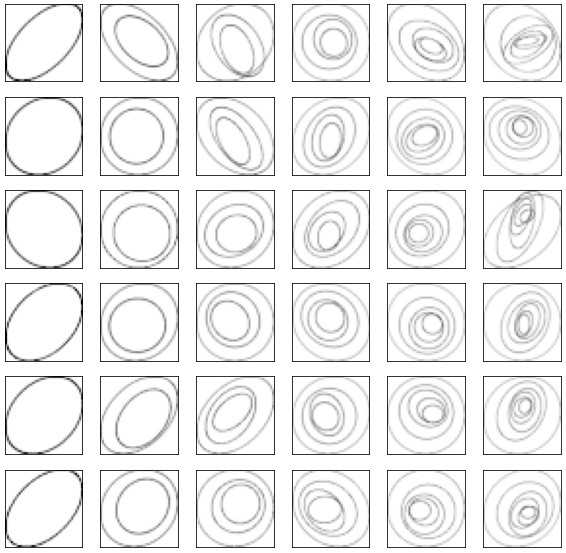
\includegraphics[width=0.5\textwidth]{nested_ellipses.PNG}
    \caption{Sample of the artificial nested ellipses datasets. First column is taken from the first dataset with 1 ellipse, second columns from the second dataset with 2 nested ellipses, until the sixth column with 6 nested ellipses.}
\end{figure}

\begin{table}[h] \label{table1}
  \centering
  \caption{Mean density with the number of nested ellipses. The density has been calculated by averaging the ratio of non-null pixel per images over 100 generated pictures for each dataset sharing the same number $n_{ellipses}$ of nested ellipses.}
  \renewcommand{\arraystretch}{1.5} % Modify the row height
  \begin{tabular}{|c|c|c|c|c|c|c|}
    \hline
    $n_{ellipses}$ & 1 & 2 & 3 & 4 & 5 & 6 \\
    \hline
    $Density$ ($\%$) & 29.0 & 51.4 & 64.3 & 70.9 & 73.5 & 75.0 \\
    \hline
  \end{tabular}
\end{table}


% Note that in this section, we study the time performance of the algorithm with no concern about convergence nor convergence speed, therefore MAM has not been fully optimized in term of convergence: $\rho$ has been set to 100 for every datasets.
% %, as this seems to be a mean value of the optimized hyperparameter. 
% No further refinement have been conducted. 
In this first experiments we analyze the impact over MAM caused by the sparsity and number of measures. We have set $\rho=100$ without proper tuning for every dataset. The study has been carried out with one processor to avoid CPU communication management.\\


% graphs of the results
\begin{figure} \label{surface}
    \centering
    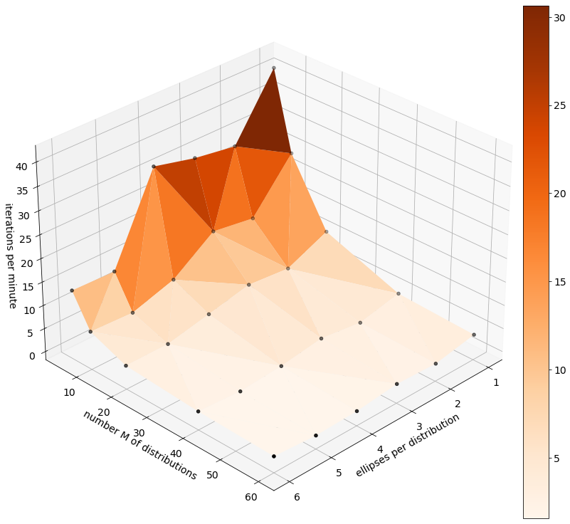
\includegraphics[width=0.8\textwidth]{surface_influence_parameters.png}
    \caption{Evolution of the number of iterations per minute depending on the density or the number of distributions.}
\end{figure}

\cref{surface} shows that, as expected, the execution time of an iteration increases with increasing density and number of measures.
% But decay rate is stronger with the dependency of the number of ellipses per distribution, it induces 
When compared to density it can be seen that the number of measures has greater influence on the method's speed (such a phenomenon can be due to the $numpy$ matrix management). 
%This can be explained by the fact that \textit{Step 2} is computed using $numpy$ that parallelize the vectorized projections of the columns of each marginal matrices before iterating to the next distribution matrice (in the \textit{for loop}). Therefore this result can be slightly different if another way of coding is taken into account, but such a way would be less efficient : $Matlab$ or $C$ can also take advantage of this intern parallelizable algebric step with vectorized matrices. [REFERENCE CODE PYTHON GITHUB ?] \\
% We underline that the number of distribution treated has an expected impact on the computation performances while the density of the support has little impact. 
This means the quantity of information in each measure does not seem to make the algorithm less efficient in term of speed. Such a result is to be put in regard with algorithms such as B-ADMM \cite{J.Ye} that are particularly shaped for sparse dataset but less efficient for denser ones.  This is a significant point that will be further developed in \cref{infl_support}.\\


\subsection{Comparison with IBP}
The Iterative Bregman Projection (IBP) \cite{IBP} is a state-of-the-art algorithm for computing Wasserstein barycenters. As mentionned in the Introduction, IBP employes a regularizing function parametrized by $\lambda>0$.
% IBP 
% %is based on an entropic regularization of the problem, and 
% can be rephrased into a two step iterative algorithms, where one step is the free-space move in the dual space, and the other is the Bregman projection in the primal space. The main idea, to make this iterative algorithm a reformulation of the initial problem, is in fact to transform the problem thanks to a penalization tuned with an hyperparameter $\lambda$, making IBP an inexact approach (see \cref{introduction}). 
The greater the $\lambda$, the worst the approximation. But in practice, $\lambda$ has to be kept in a moderate magnitude to avoid numerical errors (double-precision overflow). IBP is very sensitive to $\lambda$, that strongly relies on the dataset at stake. Thus IBP is an inexact method, whereas MAM is exact. Although the study below shows certain advantages of MAM, we make it clear that the aim is not to demonstrate which algorithm is better in general but instead to highlight the differences between the two methods and their advantages depending on the use. Note that the code for IBP is inspired from the original \cite{IBP_github}.

\subsubsection{Qualitative comparison} \label{qualitative_sec}
Here we use 100 images per digit of the MNIST database \cite{MNIST_database} where each digit has been randomly translated and rotated. Each image has 40 $\times$ 40 pixels and can be treated as probability distributions thanks to a normalization, where the pixel location is the \textit{support} and the pixel intensity the \textit{probability}. In \cref{barycenter_evolution}, we display intermediate barycenter solutions for digits $3, 4, 5$ at different time steps both for MAM and IBP. For the two methods the hyperparameters have been tuned: 
%. In the case of IBP, the larger is $\lambda$ the closer is the obtained solution to the exact solution \cite{J.Ye}
for instance, $\lambda = 1700$ is the greatest lambda that enables IBP to compute the barycenter of the 3's dataset without double-precison overflow error. Regarding MAM, a range of values for $\rho>0$ have been tested for 100 seconds of execution, to identify which one provides good performance (for example, $\rho=50$ for the dataset  of $3$'s).

% graphs of the results
\begin{figure}[h!] \label{barycenter_evolution}
    \centering
    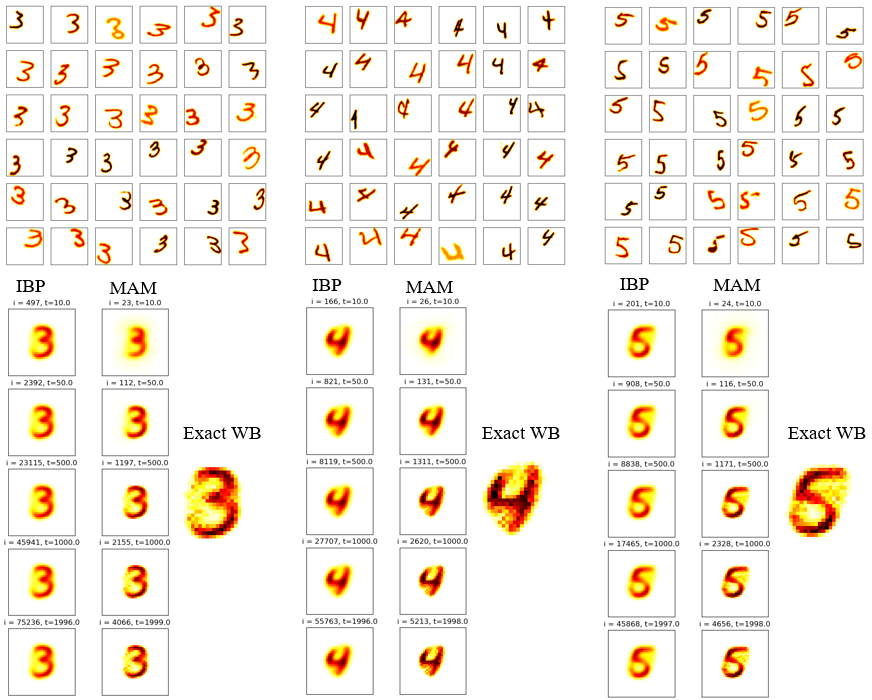
\includegraphics[width=1\textwidth]{qualitative_345.png}
    \caption{(top) For each digit 36 out of the 100 scaled, translated and rotated images considered for each barycenter. (bottom) Barycenters after $t = 10, 50, 500, 1000, 2000$ seconds, where the left-hand-side is IBP evolution of its barycenter approximation, the middle panel is MAM evolutions using 10 CPU
    and the right-hand-side is the exact solution computed by applying \textit{Gurobi} to the LP \cref{HugeLP}.}
\end{figure}

As illustrated in \cref{barycenter_evolution}, for each dataset, IBP gets quickly to a stable approximation of a barycenter. Such a point is obtained shortly after with MAM (less than 5 to 10 seconds after) but MAM continues to converge toward a sharper solution (closer to the exact solution as exemplified quantitatively in \cref{quantitative_section}). It is clear that the more CPUs used for MAM the better. We have limited the study to a dozen of CPU to allow the reader to reproduce the experimentations. While IBP is not well shaped for CPU parallelization  \cite{IBP_github, IBP, J.Ye}, MAM offers a clear advantage depending on the hardware at stake.


\subsubsection{Quantitative comparison} \label{quantitative_section}
Next we benchmark MAM, randomized MAM and IBP on a dataset with 60 images per digit of the MNIST database \cite{MNIST_database} where every digit is a normalized image 40 $\times$ 40 pixels. 
% This corresponds to a limit to compute the exact solution with a Linear Program (LP) with 150Gb RAM [INFORMATION CORRECT ON THE DIGITAL SANDBOX?? cf lscpu], using \textit{scipy.optimize.linprog} on \textit{python}.
First, all three methods have their hyperparameters tuned thanks to a sensitivity study as explained in \cref{qualitative_sec}. Then, at every time step an approximation of the computed barycenter is stored, to compute the error $\bar W_2^2(p^{k}) -\bar W_2^2(p_{exact}) := \sum_{m=1}^M \frac{1}{M}{\tt OT}(p^k,q^{(m)}) - \sum_{m=1}^M \frac{1}{M}{\tt OT}(p_{exact},q^{(m)})$.
% % The distances  $W_2^2(\mu^{(k)}, \nu^{(m)})$ between the intermediate barycenter and the distributions at stakes are calculated thanks to an LP and uniformly averaged to get the exact barycentric distance defined as $\bar W_2^2(\mu^{k}) := \frac{1}{M} \sum_{m=0}^M W_2^2(\mu^k, \nu^{(m)})$.
% The Linear Program to compute the exact value of \cref{ordonnee} uses the HIGHS method \cite{huangfu2018parallelizing} implemented with \textit{scipy} in \textit{python}. The resolution for $M=60$ exploited the total memory of our computer, thus imposing serious limitations on the number of measures that can be dealt with and if one aim at higher dimensions, computing the barycenter via an LP is out of reach \footnote{\textit{Gurobi} can be used to push the limit a bit as exemplified in \cref{qualitative_sec}.}.\\
All methods were implemented in $python$ using a \textit{MPI} based parallelization. Note that IBP is inspired from the code of G. Peyré \cite{IBP_github}, MAM from \cref{alg} and MAM-randomized (\cref{rem:random}) has only one distribution treated by processor. 
%The influence of the number of processors is studied by carrying out computations with varying numbers of processors.
%computations with varying number of processors
% The influence of the number of processors is studied using CPU.
\cref{IBP_vs_MAM} displays the evolution w.r.t time, of the error measure $\bar W_2^2(p^{k}) -\bar W_2^2(p_{exact})$, with $p_{exact}$ an exact barycenter obtained by solving LP \cref{HugeLP} directly.


% graphs of the results
\begin{figure}[h!] \label{IBP_vs_MAM}
    \centering
    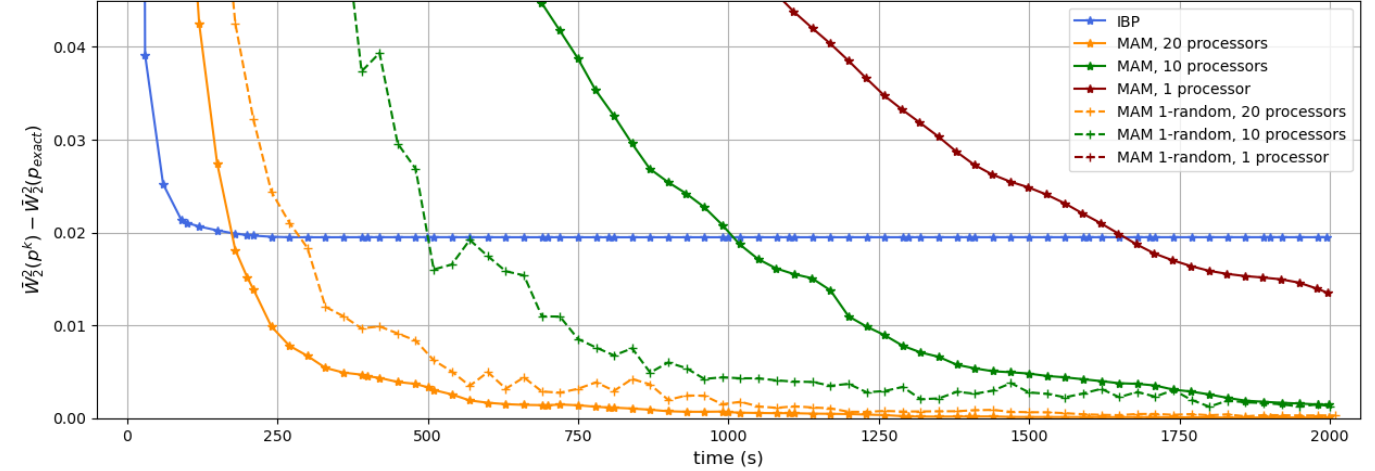
\includegraphics[width=1\textwidth]{IBP_vs_MAM.png}
    \caption{Evolution with respect to time of the difference between the Wasserstein barycenter distance of an approximation, $\bar W_2^2(p^{k})$, and the Wasserstein barycentric distance of the exact solution $\bar W_2^2(p_{exact})$ given by the LP. The time step between two points is 30 seconds.}
\end{figure}

It is clear that IBP is almost 10 time faster per iteration.
%, but being faster in one iteration does not mean faster speed overall.
However IBP computes an exact solution of an approximated problem that is tuned through the hyperparameter $\lambda$ (see \cite{IBP}). Therefore it is natural to witness IBP converging to a solution to the approximated problem, but not to an exact WB. While MAM does converge to an exact solution. So there is a threshold where the accuracy of MAM exceeds IBP: in our case, around 200s - for the computation with the greatest number of processors (see \cref{IBP_vs_MAM}).
% As expected, the more processors, the quicker the algorithm converges to a solution. Note that for every number of processors, the method converge to the same solution. Therefore the threshold where MAM becomes more accurate than IBP 
Such a treshold always exists depending on the computational means (hardware).\\
This quantitative study explains what have been exemplified with the images of \cref{qualitative_sec}: the accuracy of IBP is bounded by the choice of $\lambda$, itself bounded by an overflow error, while MAM hyperparameters only impact the convergence speed and the algorithm is always improving towards an exact solution. For this dataset, the WB computed by IBP is within 2$\%$ of accuracy and thus reasonably good. However, as shown in Table 1 in \cite{J.Ye}, one can choose other datasets where IBP's accuracy might be unsatisfactory.\\
% : \wlo{Table I in \cite{J.Ye} shows errors of approximately 20$\%$, while for such a dataset, MAM has the same behavior than exemplified above and quickly reaches an accurate solution (\cref{BADMM_vs_MAM} elaborates more precisely about MAM performances on this dataset).} \\
\\
Furthermore, \cref{IBP_vs_MAM} exemplifies an interesting asset of randomized variants of MAM: for some configurations randomized-MAM is more efficient than (deterministic) MAM but for others, the latter seems to be more effective.
Note that the curve \textit{MAM 1-random, 1 processor} does not appear on the figure: this is because it is above the y-axis value range due to its bad performance.
Indeed, there is a trade-off between time spent per iteration and precision gained after an iteration. For example, with 10 processors, each processor treats 6 measures in the deterministic MAM but only one is treated in the randomized MAM. Therefore, the time spent per iteration is roughly six time shorter in the latter and this counterbalances the loss of accuracy per iterations. On the other hand, when using 20 processors, only 3 measures are treated by each processor and the trade-off is not worth it anymore: the gain in time does not compensate for the loss in accuracy per iteration. One should adapt the use of the algorithm with care since this trade-off conclusion is only heuristic and strongly depends on the dataset and hardware at use. A sensitivity analysis is always a good thought for choosing the most effective amount of measures handled per processor while using the randomized-MAM against the deterministic MAM.

\subsubsection{Influence of the support} \label{infl_support}
This section is echoing \cref{parametric_section} and studies the influence of the support size. To do so, two datasets have been tested for MAM and IBP. The first dataset is already used in \cref{quantitative_section}: 60 pictures of 3's taken from the classic MNIST database \cite{MNIST_database}. The second dataset is also composed by these 60 images but each digit has been randomly translated and rotated in the same way as in \cref{barycenter_evolution}. Therefore, the union of the support of the second dataset is greater than the first one, as illustrated in \cref{fig_support}.

\begin{figure}[h] \label{fig_support}
    \centering
    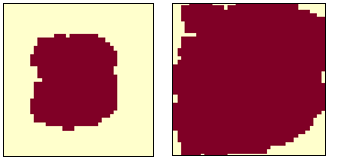
\includegraphics[width=0.5\textwidth]{support_datasets.png}
    \caption{Images with $40 \times 40$ pixel grid, where the red represents the pixels which are in the union of the dataset support composed with 60 images. (left) for the standard MNIST, (right) for the randomly translated and rotated MNIST.}
\end{figure}

\cref{fig_compare_support} presents two graphs that have been obtained just as in \cref{quantitative_section}, but displaying the evolution w.r.t time in percentage: $\Delta W_{\%} := \frac{\bar W_2^2(p^{k}) -\bar W_2^2(p_{exact}) }{\bar W_2^2(p_{exact})} \times 100$. Once more, the hyperparameters have been fully tuned. The hyperparameter of the IBP method is smaller for the second datacase. Indeed, as stated in \cite{J.Ye}, the greater is the support, the stronger are the restrictions on $\lambda$. And since the smaller is $\lambda$ the further is the approximated problem to the exact one this is expected to witness rising differences between on the following graphs. 
%As suggested in \cite{J.Ye}, this numerical difficulty can be partly addressed by treshholding entries that are too small and active research is carried in this direction but won't be deepen here.\\


% results
\begin{figure}[h] \label{fig_compare_support}
    \centering
    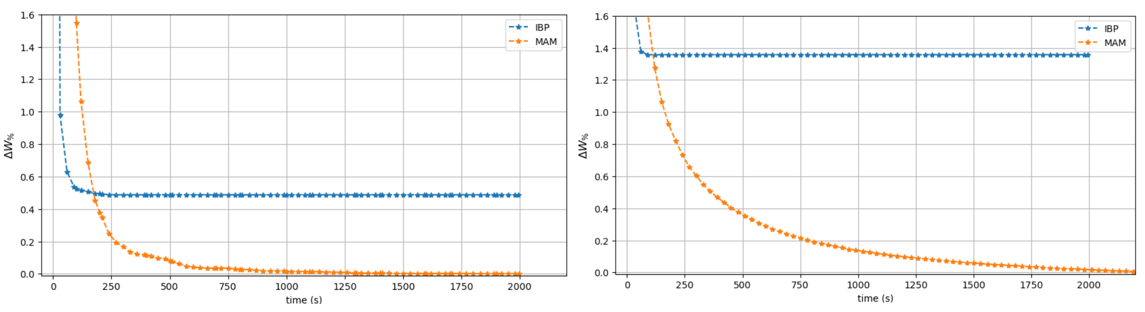
\includegraphics[width=1\textwidth]{IBP_vs_MAM_support_pourcentage.png}
    \caption{Evolution of the percentage of the distance between the exact solution of the barycenter problem and the computed solution using IBP and MAM method with 20 processors: (left) for the standard MNIST, (right) for the randomly translated and rotated MNIST. %\wlo{Ce graphique a des ordonnées en pourcentages pour comparer : c'est logique. Le graph d'au dessus à des ordonnées en valeurs absolu pour 'cacher' les faibles pourcentages, qu'en pensez vous ? Je devrais peut être tout mettre en pourcentage non?} 
    }
\end{figure}

Being an exact method, MAM is insensitive to support size. The density of the dataset has little impact on the convergence time as explained in \cref{parametric_section} and exemplified in \cref{fig_compare_support}. 
%IBP does not converge to the exact solution and because of the hyperparameter limitation, the larger is the support and the farther is the converged approximation. This is critical in the second case scenario where the approximation is almost four time farther than with the first dataset, while the support at stake is only three times larger. 
Such visual results concerning IBP initialization and parametrization have already been discussed in \cref{barycenter_evolution}, some other qualitative results can be found in \cite{Puccetti} where the author shows that properties of the distributions can be lost due to the entropy penalization in IBP.

\subsection{Comparison with B-ADMM} \label{BADMM_vs_MAM}
This subsection compares MAM with the algorithm B-ADMM of \cite{B-ADMM} using the dataset and Matlab implementation provided by the authors at the link \url{https://github.com/bobye/d2_kmeans}. We omit  IBP in our analysis because it has already been shown in  \cite[Table I]{B-ADMM} that IBP is outperformed by B-ADMM in this dataset. As in \cite[Section IV]{B-ADMM}, we consider $M=1000$ discrete measures, each with a sparse finite support set obtained by clustering pixel colors of images.
The average number of support points is around $6$, and the barycenter's number of (fixed) support points is $R=60$.
An exact WB can be computed by applying an LP solver to the extensive formulation \cref{HugeLP}. Its optimal value is $712.7$, computed in $10.6$ seconds by the Gurobi LP solver. We have coded MAM in Matlab to have a fair comparison with the Matlab B-ADMM algorithm provided at the above link. Since MAM and  B-ADMM use different stopping tests, we have set their stopping tolerances equal to zero and let the solvers stop with a maximum number of iterations. \Cref{tab:MAMxBADMM} below reports CPU time in seconds and the objective values yielded by the (approximated) barycenter $\tilde p$ computed by both solvers: $\bar W_2^2(\tilde p)$.
\begin{table}[htb]
\centering
  \caption{MAM vs B-ADMM. The considered implementation of B-ADMM is the one provided by its designers without changing parameters (except the stopping set to zero and the maximum number of iterations). Both algorithms use the same initial point. The dataset is the one considered in \cite[Section IV]{B-ADMM}. The optimal value of the WB barycenter for this dataset is $712.7$, computed by Gurobi in $10.6$ seconds. }
  \label{tab:MAMxBADMM}
\begin{tabular}{|c|cc|cc|}
\hline
\multirow{2}{*}{Iterations} & \multicolumn{2}{c|}{Objective value} & \multicolumn{2}{c|}{Seconds}       \\ \cline{2-5} 
                            & \multicolumn{1}{c|}{B-ADMM}  & MAM   & \multicolumn{1}{c|}{B-ADMM} & MAM  \\ \hline
100                         & \multicolumn{1}{c|}{742.8}   & 716.7 & \multicolumn{1}{c|}{1.1}    & 1.1  \\ \hline
200                         & \multicolumn{1}{c|}{725.9}   & 714.1 & \multicolumn{1}{c|}{2.4}    & 2.2  \\ \hline
500                         & \multicolumn{1}{c|}{716.5}   & 713.3 & \multicolumn{1}{c|}{5.6}    & 5.4  \\ \hline
1000                        & \multicolumn{1}{c|}{714.1}   & 712.9 & \multicolumn{1}{c|}{11.8}   & 10.8 \\ \hline
1500                        & \multicolumn{1}{c|}{713.5}   & 712.8 & \multicolumn{1}{c|}{18.9}   & 16.2 \\ \hline
2000                        & \multicolumn{1}{c|}{713.3}   & 712.8 & \multicolumn{1}{c|}{25.1}   & 21.6 \\ \hline
2500                        & \multicolumn{1}{c|}{713.2}   & 712.8 & \multicolumn{1}{c|}{31.0}   & 27.1 \\ \hline
3000                        & \multicolumn{1}{c|}{713.1}   & 712.7 & \multicolumn{1}{c|}{39.8}   & 32.4 \\ \hline
\end{tabular}
\end{table}


The results show that, for the considered dataset, MAM and B-ADMM are comparable regarding CPU time, with MAM providing more precise results. In contrast with MAM, B-ADMM does not have (at this time) a convergence analysis. 

\if{ % following results are not worht presenting...

\Cref{tab:MAM-random} compares MAM with three random variants in a serial environment with only one processor. To this end, we have fixed the CPU time for the random variants to the values of \cref{tab:MAMxBADMM}: the first column in \cref{tab:MAM-random} is the last one in \cref{tab:MAMxBADMM}, and the last column in \cref{tab:MAMxBADMM} is the third one in \cref{tab:MAMxBADMM}.
For instance, solver MAM-50 is the random variant of \cref{alg} with $50$ measures randomly chosen at every iteration.




\begin{table}[htb]
\centering
  \caption{Comparison of MAM (deterministic) and three randomized variants on the dataset of \cite{B-ADMM}. }
  \label{tab:MAM-random}
\begin{tabular}{|c|ccccl|}
\hline
\multirow{2}{*}{Seconds} & \multicolumn{5}{c|}{Objective value}                                                                                                                \\ \cline{2-6} 
                         & \multicolumn{1}{c|}{MAM-5} & \multicolumn{1}{c|}{MAM-50} & \multicolumn{1}{c|}{MAM-100} & \multicolumn{1}{c|}{MAM-500} & MAM                        \\ \hline
1.1                      & \multicolumn{1}{c|}{723.2} & \multicolumn{1}{c|}{716.9} & \multicolumn{1}{c|}{716.5}   & \multicolumn{1}{c|}{716.6}   & 716.7                      \\ \hline
2.2                      & \multicolumn{1}{c|}{716.4} & \multicolumn{1}{c|}{713.9}  & \multicolumn{1}{c|}{714.4}   & \multicolumn{1}{c|}{714.1}   & 714.1                      \\ \hline
5.4                      & \multicolumn{1}{c|}{714.0} & \multicolumn{1}{c|}{713.3}  & \multicolumn{1}{c|}{713.3}   & \multicolumn{1}{c|}{713.2}   & 713.3                      \\ \hline
10.8                     & \multicolumn{1}{c|}{713.3} & \multicolumn{1}{c|}{712.9}  & \multicolumn{1}{c|}{712.9}   & \multicolumn{1}{c|}{712.9}   & 712.9                      \\ \hline
16.2                     & \multicolumn{1}{c|}{713.0} & \multicolumn{1}{c|}{712.8}  & \multicolumn{1}{c|}{712.9}   & \multicolumn{1}{c|}{712.8}   & \multicolumn{1}{c|}{712.8} \\ \hline
21.2                     & \multicolumn{1}{c|}{713.0} & \multicolumn{1}{c|}{712.8}  & \multicolumn{1}{c|}{712.8}   & \multicolumn{1}{c|}{712.8}   & \multicolumn{1}{c|}{712.8} \\ \hline
27.1                     & \multicolumn{1}{c|}{712.9} & \multicolumn{1}{c|}{712.8}  & \multicolumn{1}{c|}{712.8}   & \multicolumn{1}{c|}{712.8}   & \multicolumn{1}{c|}{712.8} \\ \hline
32.4                     & \multicolumn{1}{c|}{712.8} & \multicolumn{1}{c|}{712.8}  & \multicolumn{1}{c|}{712.7}   & \multicolumn{1}{c|}{712.7}   & \multicolumn{1}{c|}{712.7} \\ \hline
\end{tabular}
\end{table}
In same cases, the randomized variant performs slightly better. For instance, the variants MAM-50 and MAM-100 manage to reach the optimal value faster than the deterministic variant: see the penultimate line in \cref{tab:MAM-random}. 
}\fi

\subsection{Unbalanced Wasserstein Barycenter} \label{sec:resul-UWB}
% \wlo{Est-il necessaire de motivier une fois de plus le cas unbalanced, peut être que j'en dis trop, je voulais motiver dans le cadre applicatif ?}
% It is possible to normalize images, such as by subtracting the mean and dividing by the standard deviation (we only divide by the sum of  the pixels values in our studies), to obtain images with similar statistical properties. However, in some cases, it may not be appropriate to normalize the images or it may not be sufficient to obtain images that are visually similar. \\
% For example, consider a set of images that have different levels of contrast or brightness. Normalizing these images may not be sufficient to make them visually similar, as the differences in contrast and brightness will still be present in the normalized images. In this case, the UWB can be used to compute a barycenter image that represents the set of images, taking into account the differences in contrast and brightness. \\
% Furthermore, the UWB can be used to generate new images that are representative of the set, but with specific characteristics. For example, one can compute the UWB of a set of blurred images with different levels of blur, and then generate new images with a specific level of blur by interpolating between the blurred images and the UWB. This can be useful in applications such as deblurring or image restoration. \\
% Overall, while normalizing images can be effective in some cases, the UWB provides a more general framework for computing representative images of a set with varying characteristics.
% \\

This section treats a particular example to illustrate the interest of using UWB. The artificial dataset is composed by 50 images with resolution $80\times80$. Each image is divided in four squared. The top left, bottom left and bottom right squared are randomly filled with double nested ellipses and the top right squared is always empty as exemplified in \cref{dataset_unbalanced}. In this example, every image is normalized to depict a probability measure so that we can compare WB and UWB.

\begin{figure}[h] \label{dataset_unbalanced}
    \centering
    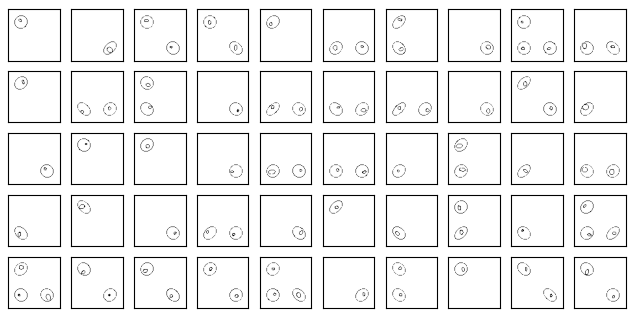
\includegraphics[width=.8\textwidth]{dataset_unbalanced_2_50pics.png}
    \caption{Dataset composed by 50 pictures with nested ellipses randomly positionned in the top left, bottom right and left corners.}
\end{figure}

With respect to \cref{UWB}, one set of constraints is relaxed and the influence of the hyperparameter $\gamma$ is studied. If $\gamma$ is large enough (i.e. greater than $\norm{{\tt vec}(d)} \approx 1000$, see \cref{prop_gamma}), the problem boils down to the standard WB problem since the example deals with probability measures: the resulting UWB is indeed a WB.  When decreasing $\gamma$ the transportation costs take more importance than the distance to $\L$ that is more and more relaxed. Therefore, as illustrated by \cref{res_gamma}, the resulting UWB splits the image in four parts, giving visual meaning to the barycenter.

\begin{figure}[h] \label{res_gamma}
    \centering
    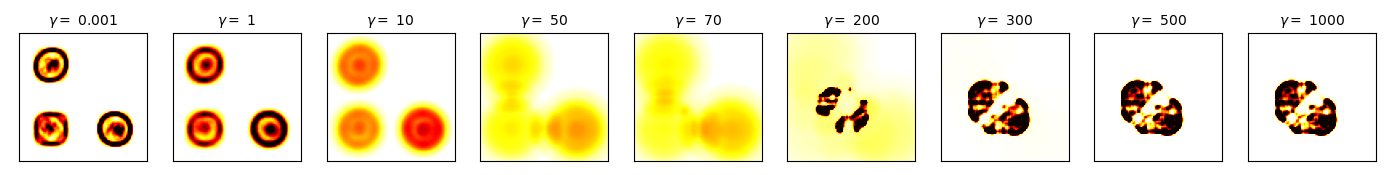
\includegraphics[width=1.\textwidth]{UWB_gamma_M50.PNG}
    \caption{UWB computed with MAM for different values of $\gamma$.}
\end{figure}


% [NOT IN THE ARTICLE]
% \cref{sec:ext} introduces the more generalized UWB problem that relaxes the constraints on $p$ and on $q^{(m)}, m=1...M$. \cref{res_eta} analyzes the impact of the newly introduced hyperparameter $\eta$ which tunes the penalization of the left constraints, while the right constraints are kept ($\gamma$ is set to a large value). Expected results are obtained: with $\eta$ tending to $0$, the transformed LP has no constraint linking $q^{(m)}$ and $\pi^{(m)} \textit{, for all } m=1...M$, therefore a straightforward solution is $\pi^{(m)}_{rs} = 0, r=1...R, s=1...S^{(m)}, m=1...M$. On the other hand, when $\eta$ is large the penalization on the left constraints is important and the UWB problem tends to the WB problem.\\
% The intermediate solutions have the same support than the WB but with reduced weights. In fact the transported distributions are no longer bounded to be the $q^{(m)}, m=1...M$, when reducing $\eta$ the transported distributions are images with support like the initial distributions but with reduced weights.

% \begin{figure}[h] \label{res_eta}
%     \centering
%     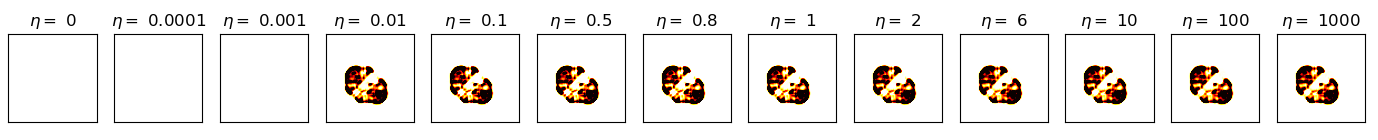
\includegraphics[width=1.\textwidth]{UWB_eta.PNG}
%     \caption{UWB computed with MAM for different hyperparameter $\gamma$.}
% \end{figure}

% \cref{res_eta_gamma} illustrates the influence of the parameters $\gamma$ and $\eta$, they must be tuned depending on the wanted behavior of the UWB. [PLUS D'EXPLICATIONS ?]

% \begin{figure}[h] \label{res_eta_gamma}
%     \centering
%     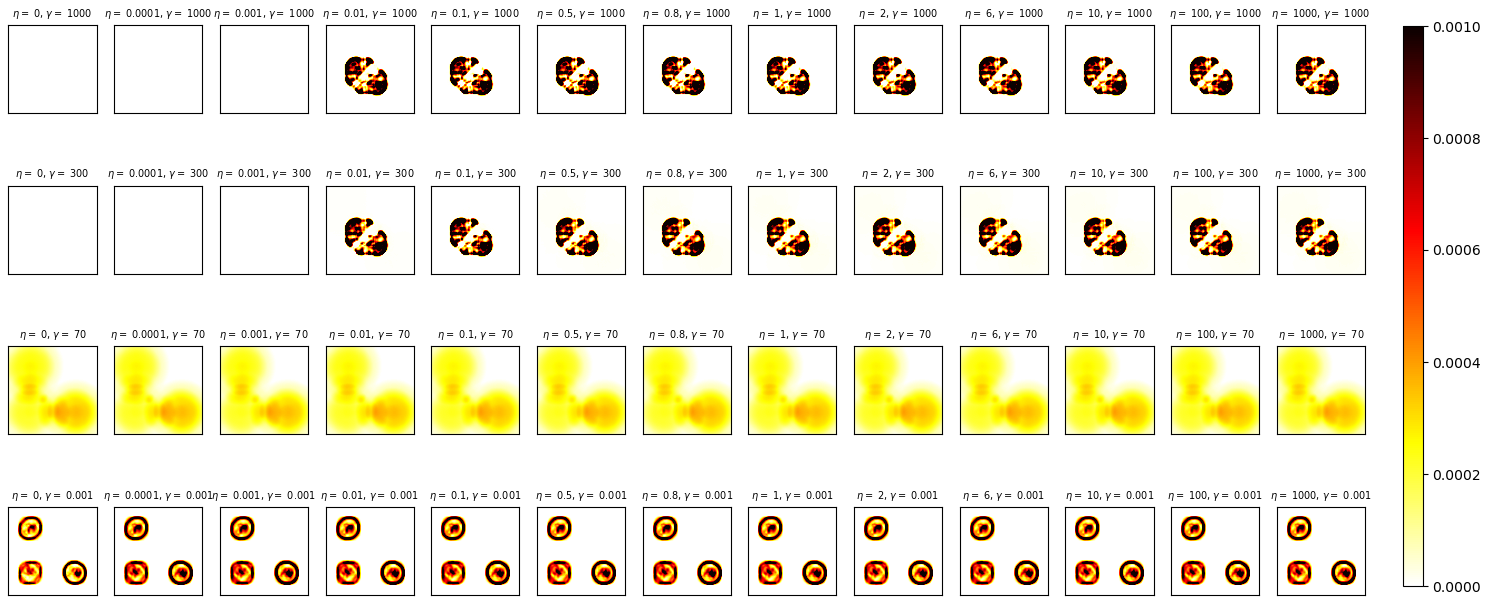
\includegraphics[width=1.\textwidth]{evolution_gamma_eta.PNG}
%     \caption{UWB computed with MAM for different hyperparameter $\gamma$.}
% \end{figure}

In the same vein, \cref{UWB_ill_MAM} provides an illustrative application of MAM for computing UWB in another dataset.

\begin{figure}[h] \label{UWB_ill_MAM}
    \centering
    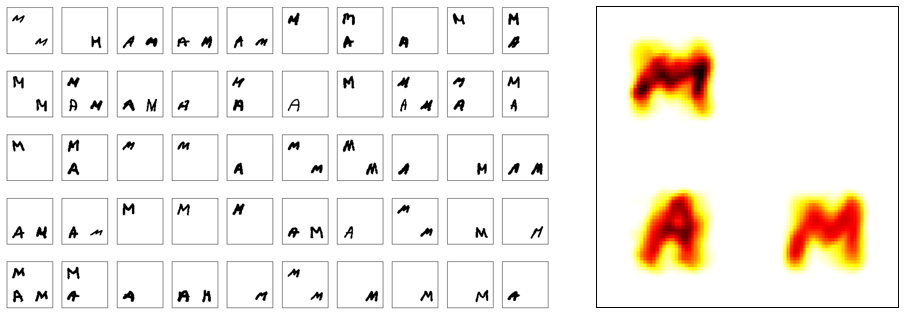
\includegraphics[width=1.\textwidth]{UWB_MAM_ill.PNG}
    \caption{\textit{(left)} UWB for a dataset of letters M-A-M built in the same logic than \cref{dataset_unbalanced} with 50 figures: \textit{(right)} resulting UWB with $\gamma=0.01$, computed in 200 seconds using 10 processors.} %en vérité 1000s mais au bout de 200 secondes on a deja ce résultat visuel
\end{figure}



% \newpage
%\section{Conclusion}

% In this study, we have presented a novel approach for computing the Wasserstein barycenter of discrete measures, leveraging the Douglas-Rachford theory. Through this innovative methodology, we have achieved convergence to the exact Wasserstein barycenter, and convergence proofs have been established based on the DR theory. \\
% Moreover, we have extended our proposed method to address the unbalanced case, resulting in the formulation of the unbalanced Wasserstein barycenter. We have introduced a new formulation of the UWB problem that relaxes only one side of the constraints, and we have further extended this definition to encompass the general case where both sides are relaxed.\\
% To assess the effectiveness of our algorithm, we conducted comprehensive comparisons against state-of-the-art methods such as IBP and B-ADMM. The results of these experiments highlighted the efficiency of MAM, which consistently converges to the exact Wasserstein barycenter. While we acknowledge that depending on the need, IBP can exhibits superior performance, these findings still support the efficacy and competitiveness of our approach.\\
% Furthermore, we have demonstrated the versatility and applicability of MAM by successfully applying it to the broader UWB problem.
% + limites


\newpage

\bibliographystyle{plain}
\bibliography{neutral_article}
% SIAM Article Template
\documentclass[review,onefignum,onetabnum]{article}
%\documentclass[article,onefignum,onetabnum]{siamonline220329} %review %article %siamonline220329

% \usepackage{a4wide}

\usepackage{amsmath,amssymb,bbm,amsthm}
\usepackage{dsfont}
\usepackage{graphicx,framed}
\usepackage{url,bm}
\usepackage{color}
\usepackage{float}
%\usepackage{algorithm}
\RequirePackage{algorithm}[0.1]
% \renewcommand{\ALG@name}{Algorithm}
\usepackage{algpseudocode} % ce package crée un petit beug de mise en page en première page
%\usepackage{algorithm2e}
%\usepackage{algorithmic}
\usepackage{subfigure}
\usepackage{epstopdf,framed}
\usepackage{mathrsfs,multirow}
\usepackage{cite}
%\usepackage[color,draft,notref]{showkeys}
\usepackage{comment}
\usepackage{xspace}
\usepackage[colorlinks=True]{hyperref}

\usepackage{xcolor}
\hypersetup{
  colorlinks,
  citecolor=blue,
  linkcolor=blue,
  urlcolor=blue}
  
\usepackage{cleveref}
\usepackage[left=2cm,right=2cm]{geometry}
\usepackage{authblk}
% Ajout de commandes pour les opérateurs différentiels et les espaces fonctionnels
\def\xd{{\textnormal{d}}}
\def\xL{{\textnormal{L}}}
\def\xW{{\textnormal{W}}}
\def\xProb{{\mathcal{P}}}
\def\xU{{\mathcal{U}}}


% wlo's definitions
%\usepackage[color,draft,notref]{showkeys}
%
\newcommand{\wlo}[1]{{\color{blue}#1}}
\renewcommand{\L}{\mathcal{B}}
\newcommand{\norm}[1]{\ensuremath{\Arrowvert #1 \Arrowvert}}
\newcommand{\inner}[2]{\langle #1, #2 \rangle}
\newcommand{\tol}{{\tt Tol }}
\newcommand{\R}{\mathds{R}}
\renewcommand{\Re}{\R}
\newcommand{\E}{\mathbb{E}}
\newcommand{\ri}[1]{{\tt ri}\,{#1}}
\newcommand{\inte}[1]{{\tt int}\,{#1}}
\newcommand{\finf}{f^{*}}
\newcommand{\dom}[1]{\mathrm{\mathcal{D}om}(#1)} %domain of an operator
\newcommand{\col}[1]{\left\{#1\right\}}
\newcommand{\croch}[1]{\left [#1\right ]}
\newcommand{\paren}[1]{\left (#1\right )}
\newcommand{\ind}{{\bf i}}
\newtheorem{claim}{Claim}
\newtheorem{myass}{Assumption}
\newtheorem{hypothesis}{Assumption}
\newtheorem{remark}{Remark}
\newtheorem{theorem}{Theorem}
\newtheorem{proposition}{Proposition}
\newtheorem{definition}{Definition}
\newtheorem{lemma}{Lemma}
\newtheorem{corollary}{Corollary}

% Information that is shared between the article and the supplement
% (title and author information, macros, packages, etc.) goes into
% ex_shared.tex. If there is no supplement, this file can be included
% directly.

%\input{ex_shared}

% Optional PDF information
% \ifpdf
% \hypersetup{
%   pdftitle={Computing Wasserstein Barycenter via operator splitting: the method of averaged marginals},
%   pdfauthor={Daniel Mimouni, Paul Malisani, Jiamin Zhu, Welington de Oliveira }
% }
% \fi

% The next statement enables references to information in the
% supplement. See the xr-hyperref package for details.

%\externaldocument[][nocite]{ex_supplement}

% FundRef data to be entered by SIAM
%<funding-group specific-use="FundRef">
%<award-group>
%<funding-source>
%<named-content content-type="funder-name"> 
%</named-content> 
%<named-content content-type="funder-identifier"> 
%</named-content>
%</funding-source>
%<award-id> </award-id>
%</award-group>
%</funding-group>

\title{Computing Wasserstein Barycenter via operator splitting: the method of averaged marginals}
\date{}
\author[1,3]{D. Mimouni\thanks{daniel.mimouni@ifpen.fr}}
\author[1]{P. Malisani\thanks{paul.malisani@ifpen.fr}}
\author[2]{J. Zhu\thanks{jiamin.zhu@ifpen.fr}}
\author[3]{W. de Oliveira\thanks{welington.oliveira@minesparis.psl.eu}}
\affil[1]{\footnotesize IFP Energies nouvelles, Dpt. Applied Mathematics, 1-4 Av Bois-Préau, 92852 Rueil-Malmaison}
\affil[2]{\footnotesize IFP Energies nouvelles, Dpt. Control and Signal Processing, 1-4 Av Bois-Préau, 92852 Rueil-Malmaison}
\affil[3]{\footnotesize Mines Paris, Center for Applied Mathematics, 1, rue Claude Daunesse, F-06904 Sophia Antipolis }
\begin{document}

\maketitle

% REQUIRED
\begin{abstract}
The Wasserstein barycenter (WB) is an important tool for summarizing sets of probabilities. It finds applications in applied probability, clustering, image processing, etc. When the probability supports are finite and fixed, the problem of computing a WB is formulated as a linear optimization problem whose dimensions generally exceed standard solvers' capabilities. For this reason, the WB problem is often replaced with a simpler nonlinear optimization model constructed via an entropic regularization function so that specialized algorithms can be employed to compute an approximate WB efficiently. Contrary to such a widespread inexact scheme, we propose an exact approach based on the Douglas-Rachford splitting method applied directly to the WB linear optimization problem for applications requiring accurate WB. 
Our algorithm, which has the interesting interpretation of being built upon averaging marginals, operates series of simple (and exact) projections that can be parallelized and even randomized, making it suitable for large-scale datasets. As a result, our method achieves good performance in terms of speed while still attaining accuracy. Furthermore, the same algorithm can be applied to compute generalized 
barycenters of sets of measures with different total masses by allowing for mass creation and destruction upon setting an additional parameter.  Our contribution to the field lies in the development of an exact and efficient algorithm for computing barycenters, enabling its wider use in practical applications. The approach's mathematical properties are examined, and the method is benchmarked against the state-of-the-art methods on several data sets from the literature.


% The Wasserstein barycenter (WB) is an important tool for summarizing sets of probabilities. It finds applications in applied probability, clustering, image processing, etc. When the probability supports are finite and fixed, the problem of computing a WB is formulated as a linear optimization problem whose dimensions generally exceed standard solvers' capabilities. For this reason, the WB problem is often replaced with a simpler nonlinear optimization model constructed via an entropy-like regularization function so that specialized algorithms can be employed to compute an approximate WB efficiently. Contrary to such a widespread inexact scheme, we propose an exact approach based on the Douglas-Rachford splitting method applied directly to the WB linear optimization problem for applications requiring accurate WB. 
% Our algorithm, which has the interesting interpretation of being built upon averaging marginals, operates a series of simple (and exact) projections that can be carried out  in parallel and even randomly. As a result, our method achieves good performance in terms of speed while still attaining accuracy. Furthermore, the same algorithm can be applied to the broader class of unbalanced WB problems upon setting an additional parameter. The approach's mathematical properties are examined, and the method is benchmarked against the state-of-the-art \emph{Iterative Bregman Projection} method on several data sets from the literature.


%We present a new algorithm for computing the exact Wasserstein barycenter of a set of empirical probability measures under the optimal transport metric. The Wasserstein measure has widespread applications in diverse fields, such as applied probability, economics, statistics, clustering, or image processing. Within this framework, the Wasserstein barycenter is an important tool for summarizing sets of probability distributions. However, computing the exact solution of the barycenter requires resolving large linear programs, which is prohibitively costly. \\
%Our proposed algorithm offers a general approach for computing both classic and unbalanced Wasserstein barycenters. It decomposes the linear program using the Douglas-Rachford method and operates two simple projections until it converges. \\
%We examine the mathematical characteristics of our method and perform experiments to demonstrate its effectiveness. \\
%Our contribution to the field lies in the development of an exact and efficient algorithm for computing the Wasserstein barycenter, enabling its wider use in practical applications. \\
%Additionally, the algorithm is parallelizable and a randomized version is also possible, making it suitable for large-scale datasets. Then, our method achieves high performance in terms of speed, compared to state-of-the-art methods while still maintaining exactness.

\end{abstract}

% REQUIRED
%\begin{keywords}
%Wassertein Barycenters, Optimal Transport, Douglas-Rachford Method
%%, Unbalanced, Image processing \and Parallel computing
%\end{keywords}

% REQUIRED
%\begin{MSCcodes}
%46N10, 90C08, 90C05, 90C25 
%\end{MSCcodes}

\section{Introduction} \label{introduction}


In applied probability, stochastic optimization, and data science, a crucial aspect is the ability to compare, summarize, and reduce the dimensionality of empirical  measures. Since these tasks rely heavily on pairwise comparisons of measures, it is essential to use an appropriate metric for accurate data analysis. 
Different metrics define different barycenters of a set of measures:  %. More precisely, 
a barycenter is a mean element that minimizes the (weighted) sum of all its distances to the set of target measures. 
When the chosen metric is the optimal transport one, and there is mass equality between the measures, the underlying barycenter is denoted by Wasserstein Barycenter (WB).

The optimal transport metric defines the so-called Wasserstein distance (also known as Mallows or Earth Mover's distance),  a popular choice in statistics, machine learning, and stochastic optimization \cite{Peyre_Cuturi_2019,Oliveira_CEPEL_2009,Pflug_Pichler_2014}.
The Wasserstein distance has several valuable theoretical and practical properties \cite{Villani_2009,Rubner_2000} that are transferred to (Wasserstein) barycenters \cite{Carlier,Cuturi_Doucet_14,Puccetti,Peyre_Cuturi_2019}.
Indeed, thanks to the Wasserstein distance, one key advantage of WBs is their ability to preserve the underlying geometry of the data, even in high-dimensional spaces. This fact makes WBs particularly useful in image processing, where datasets often contain many pixels and complex features that must be accurately represented and analyzed \cite{simon2020barycenters,tartavel2016wasserstein}. 
% For example, Wasserstein barycenters can be used in image morphing or segmentation, which involves dividing an image into multiple regions based on the similarity of the pixels within each region. By computing a WB of a set of probability measures defined over the image space, it is possible to accurately cluster similar pixels and identify the different regions of an image \cite{simon2020barycenters}.
% Image restoration is another example: WBs can remove noise and artifacts from an image while preserving important features and structures \cite{tartavel2016wasserstein}. 
 

Being defined by the Wasserstein distance, WBs are challenging to compute. The Wasserstein distance is computationally expensive because, to compute an optimal transport plan, one needs to cope with a large linear program (LP) that has no analytical solution and cubic worst-case complexity\footnote{More precisely, $O(S^3log(S))$, with $S$ the size of the input data.} \cite{J.Ye}. The situation becomes even worse for computing a WB because its definition involves several optimal transport plans. In the simpler case of fixed support, which is the focus of this work (see \cref{sec:background} below), computing a WB amounts to solving an LP whose dimensions generally exceed standard solvers' capabilities \cite{Carlier}. Several numerical methods have been proposed in the literature to address the challenge. 
They invariably fall into one of the following categories:
\begin{itemize}
    \item [i)] Inexact methods, based on reformulations via  an entropic regularization \cite{Cuturi_Doucet_14,J.Ye,Cuturi,Gramfort_Pyre_Cuturi_2015,Cuturi_Peyre_2016,IBP,Peyre_Cuturi_2019};

%\item [ii)] Inexact decomposition methods, based on approximating models (via entropy-like regularizations) and techniques of decomposition \cite{Cuturi_Doucet_14,J.Ye,Gramfort_Pyre_Cuturi_2015};


\item [ii)] Exact decomposition methods, consisting in  solving a sequence of smaller and simpler subproblems \cite{Ye_ADMM,Cuturi}.
\end{itemize}

While our proposal falls into the second category, the vast 
majority of methods found in the literature are inexact ones, employing or not decomposition techniques.  
%If we have $M$ discrete distributions, each with $S(m), m=1,\ldots,M$ support points, their actual Wasserstein barycenter can be determined using linear programming, as demonstrated in \cite{Carlier}. This is a reasonable approach since the support points of the barycenter can only exist in a finite (but still enormous) number of potential positions. Nevertheless, even for a relatively small number of distributions with just 10 support points each, solving the real discrete barycenter quickly becomes impractical. \\
Indeed, the work \cite{Cuturi} proposes to inexactly compute a WB by solving an approximating model obtained by regularizing the WB problem with  an entropy-like function. 
The technique allows one to employ the celebrate Sinkhorn algorithm \cite{Sinkhorn_1974,Cuturi_2013}, which  has a simple closed-form expression and can be implemented  efficiently using only matrix operations. When combined with a projected subgradient method, this regularizing approach fits into category i) above. However, if instead the underlying transport subproblems are solved exactly without the regularization technique, then Algorithm 1 from \cite{Cuturi} falls into category ii).
%that exploits the structure of the Wasserstein metric to avoid computing expensive pairwise distances between distributions. Instead, it iteratively rescales the rows and columns of a cost matrix to enforce a balance constraint. 
%In this setting, \cite{Cuturi} approximates the optimal transport plan with the Sinkhorn subgradient method to compute the Wasserstein barycenter of a set of probability measures. 
%Cuturi's work on the Sinkhorn algorithm has had a profound impact on the field of optimal transport and has enabled the computation of Wasserstein barycenters on large-scale datasets. 
%The algorithm has been used in a wide range of applications, including image processing, machine learning, and neuroscience.  \\

The regularization technique of \cite{Cuturi_2013} opened the way to the \emph{Iterative Bregman Projection} (IBP) method proposed in \cite{IBP}. 
IBP is highly memory efficient for distributions with shared support set and is considered to be one of the most effective methods to tackle WB problems.
However, as IBP works with an approximating model, the computed point is not a solution to the WB problem, and thus IBP is an inexact method. 

Another approach fitting into the category of inexact methods
has been recently proposed in \cite{J.Ye}, which uses the same type of regularization as IBP but decomposes the problem into a sequence of smaller subproblems with straightforward solutions. More specifically, the approach in \cite{J.Ye} is an modification (tailored to the WB problem) of the \emph{Bregman Alternating Direction Method of Multipliers} (B-ADMM) of \cite{B-ADMM}. 
The modified B-ADMM  has been shown to compute promising results for sparse support measures and therefore is well-suited in some clustering applications. However, 
the theoretical convergence properties of the modified B-ADMM algorithm is not well understood and the approach should be considered as an heuristic.
%While the IBP method is often more advised because the theoretical convergence property of the modified B-ADMM algorithm is not well understood. \\

An inexact method that disregards entropic regularizations is presented \cite{Puccetti}, and denoted  by \emph{Iterative Swapping Algorithm} (ISA).
The approach is a non-parametric algorithm that provides a
sharp image of the support of the barycenter and has a quadratic time complexity.
Essentially, ISA is designed upon  approximating the linear program by a multi-index assignment problem which is solved in an iterative manner. 
% Note that an alternative of this algorithm is proposed in the conclusion of the same article \cite{Puccetti} to compute the exact WB in certain cases, but this implies skyrocketting the time and storage complexity. 
Another approach based on successive approximations of the WB (linear programming) problem is proposed in \cite{Borgwardt_2022}.

Concerning exact methods, the work \cite{Carlier_Oberman_Oudet_2015} proposes a simpler linear programming reformulation of the WB problem that leads to an LP that scales linearly with the
number of measures. Although the resulting LP is smaller than the WB problem, it still suffers from heavy computation time and memory consumption \cite{Puccetti}.
In contrast, \cite{Ye_ADMM} proposes to address the WB problem via the standard ADMM algorithm, which decomposes the problem in smaller and simpler subproblems. As mentioned by the authors in their subsequent paper \cite{J.Ye}, the numerical efficiency of the standard ADMM is still inadequate for large datasets.


%All the methods mentioned in the above references deal exclusively with sets of probability measures. The reason is that WBs are limited to measures with equal total masses. As mentioned in \cite{Heinemann_Klatt_Munk_2022}, the difference in total mass intensity is crucial in many real-life applications. Therefore, normalizing general positive measures to compute a standard  WB is generally unsatisfactory and limits the use of WBs in practical applications. Within this framework, generalized barycenters \cite{Heinemann_Klatt_Munk_2022,Sejourne_Peyre_Vialard_2023} are extensions of the standard WB to summarize measures with different total masses.
%This notion is particularly useful in image-processing applications involving comparing and fusing different properties. For example, some applications can be found in medical imaging where it is often necessary to compare images from different patients \wlo{REF}. It is also used in object detection to consider brightness or contrast in images \wlo{REF}. 
All the methods mentioned in the above references deal exclusively with sets of probability measures because WBs are limited to measures with equal total masses. A tentative way to circumvent this limitation is to normalize general positive measures to compute a standard WB. However, such a naive strategy is generally unsatisfactory and limits the use of WBs in many real-life applications such as logistic, medical imaging and others coming from the field of biology \cite{Heinemann_Klatt_Munk_2022,Sejourne_Peyre_Vialard_2023}. 
Consequently, the concept of WB has been generalized to summarize such more general measures. Different generalizations of the WB exist in the literature, and they are based on variants of \emph{unbalanced optimal transport problems} that define a distance between general non-negative, finitely supported measures by allowing for mass creation and destruction \cite{Heinemann_Klatt_Munk_2022}. Essentially, such generalizations, known as unbalanced Wasserstein barycenters (UWBs), depend on how one chooses to relax the marginal constraints. In the review paper \cite{Sejourne_Peyre_Vialard_2023} and references therein, marginal constraints are moved to the objective function with the help of divergence functions. Differently, in \cite{Heinemann_Klatt_Munk_2022} the authors replace the marginal constraints with sub-couplings and penalize their discrepancies. It is worth mentioning that UWB is more than simply copying with global variation in the measures' total masses. Generalized barycenters  tend to be more robust to local mass variations, which include outliers and missing parts \cite{Sejourne_Peyre_Vialard_2023}.

For the sake of a unified algorithmic proposal for both balanced and unbalanced WBs, in this work, we consider a different formulation for dealing with sets of measures with different total masses. 
% Instead of relaxing both marginal constraints in each one of the underlying optimal transportation subproblems as done in \cite{Heinemann_Klatt_Munk_2022,Sejourne_Peyre_Vialard_2023} and references therein, our formulation generalizes the balanced WB by relaxing the constraint that the barycenter is a marginal measure of all underlying transportation plans. 
While our approach can be seen as an abridged alternative to the thorough methodologies of \cite{Heinemann_Klatt_Munk_2022} and \cite{Sejourne_Peyre_Vialard_2023}, its favorable structure for efficient splitting techniques combined with the good quality of the issued UWBs confirm the formulation's practical interest.


%In this work, we propose a distributed algorithm for computing barycenters in the case of finite and fixed support data. Our approach, which falls into the category  of exact decomposition methods, builds upon the celebrated  Douglas-Rachford splitting operator method (DR) \cite{Douglas_Rachford_1956,Eckstein_Bertsekas_1992,Accelerated_DR_2020} and is denoted by \emph{Method of Averaged Marginals} (MAM). 

To cope with the challenge of computing (balanced and unbalanced) WBs, we propose a new algorithm based on the celebrated 
Douglas-Rachford splitting operator method (DR) \cite{Douglas_Rachford_1956,Eckstein_Bertsekas_1992,Accelerated_DR_2020}. Our proposal, which falls into the category  of exact decomposition methods, is denoted by \emph{Method of Averaged Marginals} (MAM). The motivation 
for its name is due to the fact that, at every iteration, 
the algorithm computes a barycenter approximation by 
averaging marginals issued by transportation plans that are 
updated independently, in parallel, and even randomly if necessary. 
Accordingly, the algorithm operates a series of simple and exact projections that can be carried out in parallel and even randomly.
%
%Due to the DR's versatility and 
Thanks to our unified analysis,  MAM can be applied to both balanced and unbalanced WB problems without any change: all that is needed is to set up a parameter.
To the best of our knowledge, MAM is the first approach capable of handling balanced and unbalanced WB problems in a single algorithm, which can be further run in a deterministic or randomized fashion.

 In addition to its versatility, MAM copes with scalability issues arising from barycenter problems, is memory efficient, and has convergence guarantees to an exact barycenter. 
Although MAM's convergence speed is not as exceptional as IBP's, it is observed in practice that after a few tens of iterations, the average of marginals computed by MAM is a better approximation of a WB than the solution provided by IBP, no matter how many iterations the latter performs\footnote{The reason is that IBP converges fast but to the solution of an approximate model, not to an exact WB.}.
As further contributions, we conduct experiments on several data sets from the literature to demonstrate the computational efficiency and accuracy of the new algorithm and make our Python codes publicly available at the link (\url{https://ifpen-gitlab.appcollaboratif.fr/detocs/mam_wb}).
 
The remainder of this work is organized as follows. \Cref{sec:background} introduces the notation
and recalls the balanced WB problems’ formulation.
The proposed formulation for unbalanced WBs is presented in \cref{sec:UWB}.
In \cref{sec:DR} the WB problems are reformulated in a suitable way so that the Douglas-Rachford splitting (DR) method can be applied. The same section briefly recalls the DR algorithm and its convergence properties both in the deterministic and randomized settings. The main contribution of this work, the Method of Averaged Marginals, is presented in \cref{sec:MAM1}.
Convergence analysis is given in the same section by relying on the DR algorithm's properties.
\Cref{sec:num} illustrates the
numerical performance of the deterministic and randomized variants of MAM on several data sets from the literature. Numerical comparisons with IBP and B-ADMM are presented for the balanced case. Then some applications of the UWB are considered. 



\section{Background on optimal transport and Wasserstein barycenter}\label{sec:background}

Let $(\Omega,\mathtt{d})$ be a metric space and $P(\Omega)$ the set of Borel probability measures on $\Omega$. 
Furthermore, let $\xi$ and $\zeta$ be two random vectors having probability measures $\mu$ and $\nu$ in  $P(\Omega)$, that is, $\xi\sim \mu$ and $\zeta\sim \nu$. 
%For any point $\mu \in \Omega$, $\delta_\mu$ is the Dirac unit mass on $\mu$. 

\begin{definition}[Wasserstein Distance]
For $\iota \in [1, \infty)$, and probability measures $\mu$ and $\nu$ in  $P(\Omega)$. Their $\iota$-Wasserstein distance $W_\iota$ is :
\begin{equation}\label{WD}
\tag{WD}
W_\iota(\mu,\nu):=\left(\inf_{\pi \in U(\mu,\nu)} \int_{\Omega\times \Omega} \mathtt{d}(\xi,\zeta)^\iota d\pi(\xi,\zeta)\right)^{1/\iota},
\end{equation}
where $U(\mu,\nu)$ is the set of all probability measures on $\Omega\times \Omega$ having marginals $\mu$ and $\nu$. 
We denote by $W_\iota^\iota(\mu,\nu)$, $W_\iota$ to the power $\iota$ , i.e.  $W_\iota^\iota(\mu,\nu) := (W_\iota(\mu,\nu))^\iota$. 
\end{definition}
Throughout this work, for $\tau\geq 0$ a given scalar, the notation $\Delta_n(\tau)$ denotes the set of non-negative vectors in $\R^n$ adding up to $\tau$, that is,
\begin{equation}\label{eq:Delta}
\Delta_n(\tau):=\col{u \in\R^n_+:\; \sum_{i=1}^nu_i=\tau}.
\end{equation}
If $\tau=1$, then $\Delta_n(\tau)$, denoted simply by $\Delta_n$, is the $n+1$ simplex.

\begin{definition}[Wasserstein Barycenter]
Given $M$ measures
$\{\nu^{(1)},\ldots,\nu^{(M)}\}$ in $ P(\Omega)$ and $\alpha \in \Delta_M$, an $\iota$-\emph{Wasserstein barycenter} with weights $\alpha$ 
 is a solution to the following optimization problem
\begin{equation}\label{WB}
%\tag{WB}
\min_{\mu \in P(\Omega)}\; \sum_{m=1}^M \alpha_m W_\iota^\iota(\mu,\nu^{(m)})\,.
\end{equation}
%(In general, one takes $\alpha_m=\frac 1M$ for all $m=1,\ldots,M$ in the above definition.)
\end{definition}
%A WB exists in generality and is unique should the measures $\nu^{(j)}$ be absolutely continuous \cite{Carlier}.

A WB $\mu$ exists in generality and, if one of the $\nu^{(m)}$ vanishes on all Borel subsets of Hausdorff dimension $dim(\Omega)-1$, then it is also unique \cite{Carlier}. If the measures are discrete, then uniqueness is no longer ensured in general.

%\subsection{Restriction to Empirical Measures}

\subsection{Discrete Wasserstein Barycenter}
This work focus on empirical measures based on finitely many $R$ scenarios $\Xi:=\{\xi_1,\ldots,\xi_R\}$ for $\xi$ and  $S^{(m)}$ scenarios \newline 
$Z^{(m)}:=\{\zeta^{(m)}_1,\ldots,\zeta^{(m)}_{S^{(m)}}\}$ for $\zeta^{(m)}$, $m=1,\ldots,M$, i.e., measures of the form
\begin{equation}\label{eq:empirical}
\mbox{$\mu=\sum_{r=1}^R p_r\delta_{\xi_r}$ \quad and \quad   $\nu^{(m)}=\sum_{s=1}^{S^{(m)}} q^{(m)}_s\delta_{\zeta^{(m)}_s}$,\quad $m=1,\ldots,M$,}
\end{equation}
with $\delta_u$ the Dirac unit mass on $u \in \Omega$, $p \in \Delta_R$, and $q^{(m)}\in \Delta_{S^{(m)}}$, $m=1,\ldots,M$.

%Let the supports $\Xi$ and $Z^{(m)}$ of the empirical measures $\mu$ an $\nu^{(m)}$, $m=1,\ldots,M$, be fixed. 
In this setting, when the support $\Xi$ is fixed, the $\iota$-Wasserstein distance $W_\iota(\mu,\nu)$ of two empirical  measures $\mu$ and $\nu^{(m)}$  is the $\iota^{th}$ root of the optimal value of the following LP, known as \emph{optimal transportation} (OT) problem
\begin{equation}\label{OT}
%\tag{OT}
%{\tt OT}(p,q;{\xi,\zeta})=
{\tt OT}_{\Xi}(p,q):=
\left\{
\begin{array}{lll}
\displaystyle \min_{\pi\geq 0} & \displaystyle  \sum_{r=1}^R \sum_{s=1}^{S} \mathtt{d}(\xi_r,\zeta_s)^\iota\pi_{rs}\\
\mbox{s.t.}& \sum_{r=1}^R \pi_{rs} = q_s,& s=1,\ldots,S\\
&\sum_{s=1}^{S} \pi_{rs} = p_r,& r=1,\ldots,R.
\end{array}
\right.
\end{equation}
The feasible set above is  refereed to as the \emph{transportation polytope}, issued by the so-called \emph{marginal constraints}. 
%Therefore, defined as: $U_=(\mu, \nu) = \{\pi \in \mathbb{R}_+^{R\times S} \| \pi^T \mathbbm{1}_S = p, \pi \mathbbm{1}_R = q  \}$.
An optimal solution of this problem is known as an optimal transportation plan.
Observe that a transportation plan can be represented as a matrix whose entries are non-negative, the row sum equals the marginal $q$, and the column sum equals $p$.
%that row and column marginals of every transportation plan the $R\times S$ nonnegative matrices are equals to $p$ and $q$ respectively.

\begin{definition}[Discrete Wassertein Barycenter - WB]\label{def:WB-general}
A Wassertein barycenter of a set of $M$ empirical probability measures $\nu^{(m)}$ having support $Z^{(m)}$, $m=1,\ldots,M$, is a solution to the following optimization problem
\begin{equation}\label{eq:free-WB}
\min_{\Xi,p\in \Delta_R}\;\sum_{m=1}^M \alpha_m{\tt OT}_{\Xi}(p,q^{(m)}).
\end{equation}
\end{definition}
The above is a challenging nonconvex optimization problem that is in general dealt with via block-coordinate optimization: at iteration $k$, the support is fixed $\Xi^k$, and the convex optimization problem, $\min_{p \in \Delta_R}\;\sum_{m=1}^M \alpha_m{\tt OT}_{\Xi^k}(p,q^{(m)})$,
% \[% \begin{equation}\label{eq:WB}
% \min_{p \in \Delta_R}\;\sum_{m=1}^M \alpha_m{\tt OT}_{\Xi^k,Z^{(m)}}(p,q^{(m)})
% \] %\end{equation}
is solved to define a vector $p^k$, which is in turn fixed to solve $\min_{\Xi}\;\sum_{m=1}^M \alpha_m{\tt OT}_{\Xi}(p^k,q^{(m)})$ that updates the support $\Xi^k$ to $\Xi^{k+1}$.
% \[
% \min_{\Xi}\;\sum_{m=1}^M \alpha_m{\tt OT}_{\Xi,Z^{(m)}}(p^k,q^{(m)}).
% \]
When the metric $\mathtt{d}(\cdot,\cdot)$ is the Euclidean distance and $\iota=2$, the last problem has a straightforward solution (see for instance \cite[Alg. 2]{Cuturi_Doucet_14} and \cite[\S\, II]{J.Ye}). For this reason, in the remainder of this work we focus on the more challenging problem of minimizing w.r.t. the vector $p$.
%We will come back to the more general problem~\cref{eq:free-WB} in Subsection~\ref{subsec:free-WB} below.
%
\begin{definition}[Discrete Wasserstein Barycenter with Fixed Support]\label{def:WB}
A fixed-support Wasserstein barycenter of a set of $M$ empirical probabilities measures $\nu^{(m)}$ having support $Z^{(m)}$, $m=1,\ldots,M$, is a solution to the following optimization problem
\begin{equation}\label{eq:WB}
\min_{p \in \Delta_R}\;\sum_{m=1}^M \alpha_m{\tt OT}_{\Xi}(p,q^{(m)}).
\end{equation}
\end{definition}
In the above definition, the support $\Xi$ is fixed and the optimization is performed with respect  to the vector $p$. Our approach to solve \cref{eq:WB} 
% It is not difficult to see that ${\tt OT}_{\Xi}$ is a convex function on argument $p$. Therefore, \cref{eq:WB} is a convex optimization problem having a hard-to-evaluate objective function: $M$ transportation problems must be solved to compute the functional value for a given vector $p \in \Delta_R$. Such a decomposable structure has already been exploited in \cite{Cuturi_Doucet_14}. To avoid solving $M$ transportation problems per iteration, we take a different path that 
can be better motivated after writing down
the extensive formulation of the problem.
Indeed, looking for a barycenter $\mu$ with fixed atoms $\xi$ and probability $p$ is equivalent to solving the following huge-scale LP, where we denote $\mbox{$d^{(m)}_{rs}:=\alpha_m\mathtt{d}(\xi_r,\zeta^{(m)}_s)$ ($r=1,\ldots,R$, $s=1,\ldots,S^{(m)}$, $m=1,\ldots,M$):}$

% \[\mbox{$d^{(m)}_{rs}:=\alpha_m\mathtt{d}(\xi_r,\zeta^{(m)}_s)$ ($r=1,\ldots,R$, $s=1,\ldots,S^{(m)}$, $m=1,\ldots,M$):}\]

\begin{equation}  \label{HugeLP}
\left\{
\begin{array}{llllllllll}
\displaystyle \min_{p,\pi} & \displaystyle \sum_{r=1}^R \sum_{s=1}^{S^{(1)}} d^{(1)}_{rs}\pi^{(1)}_{rs}&+\cdots +& \displaystyle\sum_{r=1}^R
 \sum_{s=1}^{S^{(M)}} d^{(M)}_{rs}\pi^{(M)}_{rs}\\
 \mbox{ }\\
 \mbox{s.t.} & \sum_{r=1}^R \pi^{(1)}_{rs} &&&\hspace{-1.3cm}= q^{(1)}_s,&\;s=1,\ldots,S^{(1)} \\
 &&\ddots &&\hspace{-1.3cm}\vdots\\
 &&&\sum_{r=1}^R \pi^{(M)}_{rs} &\hspace{-1.3cm}= q^{(M)}_s,&\;s=1,\ldots,S^{(M)}\\[1em]
 &\sum_{s=1}^{S^{(1)}} \pi^{(1)}_{rs} &&&\hspace{-1.3cm}= p_r,&\;r=1,\ldots,R\\
 &&\ddots &&\hspace{-1.3cm}\vdots\\
  &&&\sum_{s=1}^{S^{(M)}} \pi^{(M)}_{rs} &\hspace{-1.3cm}= p_r,&\;r=1,\ldots,R\\
  \\
  & p \in \Delta_R,\pi^{(1)}\geq 0&\cdots &\pi^{(M)}\geq 0,
\end{array}
\right.
\end{equation}
The constraint $p \in \Delta_R$ above is redundant and can be removed: we always have, for $m=1,\ldots,M$, $\sum_{r=1}^Rp_r = \sum_{r=1}^R\left(\sum_{s=1}^{S^{(m)}} \pi^{(m)}_{rs}\right)= \sum_{s=1}^{S^{(m)}} \left(\sum_{r=1}^R \pi^{(m)}_{rs}\right)= \sum_{s=1}^{S^{(m)}} q_s^{(m)}=1.$

% \[\sum_{r=1}^Rp_r = \sum_{r=1}^R\left(\sum_{s=1}^{S^{(m)}} \pi^{(m)}_{rs}\right)= \sum_{s=1}^{S^{(m)}} \left(\sum_{r=1}^R \pi^{(m)}_{rs}\right)= \sum_{s=1}^{S^{(m)}} q_s^{(m)}=1.\]

The dimension of the above LP is $R(1+\sum_{m=1}^M S^{(m)})$ and grows rapidly with the number of measures $M$. For instance, for moderate values such as $R=S^{(m)}=1600$, $m=1,\ldots,M$ (corresponding to figures with $40\times 40$ pixels) and $M=100$, the above LP has more than 256 millions of variables\footnote{More precisely, $ 256\,001\,600$ variables.}.


Although variable $p$ is the one of interest, 
we can remove $p$ from the above formulation and recover it easily by working with the following linear subspace.
\begin{definition}[Balanced subspace]
% Given the fixed-support Wasserstein barycenter problem~\cref{HugeLP}, 
We denote by \emph{balanced subspace} the following linear subspace of balanced transportation plans:  
\begin{equation}\label{eq:L}
\L:=\left\{\pi=(\pi^{(1)},\ldots,\pi^{(M)})\left\vert \begin{array}{lclllllll}
\sum_{s=1}^{S^{(1)}} \pi^{(1)}_{rs} &= &\sum_{s=1}^{S^{(2)}} \pi^{(2)}_{rs},& r=1,\ldots,R\\
\sum_{s=1}^{S^{(2)}} \pi^{(2)}_{rs} &= & \sum_{s=1}^{S^{(3)}} \pi^{(3)}_{rs},&r=1,\ldots,R\\
&\vdots\\
\sum_{s=1}^{S^{(M-1)}} \pi^{(M-1)}_{rs} &=&\sum_{s=1}^{S^{(M)}} \pi^{(M)}_{rs},& r=1,\ldots,R
\end{array}
\right.
\right\}.
\end{equation}
\end{definition}
The term \emph{balanced} is due to the fact that given $\nu^{(m)}$ in~\cref{eq:empirical}, $\sum_{j=1}^{S(m)}q_j^{(m)}=
\sum_{j=1}^{S(m')}q_j^{(m')}$, $ m, m'=1,\ldots,M.$
% \[\sum_{j=1}^{S(m)}q_j^{(m)}=
% \sum_{j=1}^{S(m')}q_j^{(m')}, \quad m, m'=1,\ldots,M.\]
Observe that problem~\cref{HugeLP} is equivalent, in terms of optimal value and optimal transportation plans, to the following LP
\begin{equation}  \label{HugeLP-bis}
\left\{
\begin{array}{llllllllll}
\displaystyle \min_{\pi \in \L} & \displaystyle \sum_{r=1}^R \sum_{s=1}^{S^{(1)}} d^{(1)}_{rs}\pi^{(1)}_{rs}&+\cdots +& \displaystyle\sum_{r=1}^R
 \sum_{s=1}^{S^{(M)}} d^{(M)}_{rs}\pi^{(M)}_{rs}\\
 \mbox{ }\\
 \mbox{s.t.} & \sum_{r=1}^R \pi^{(1)}_{rs} &&&\hspace{-1.3cm}= q^{(1)}_s,&\;s=1,\ldots,S^{(1)} \\
 &&\ddots &&\hspace{-1.3cm}\vdots\\
 &&&\sum_{r=1}^R \pi^{(M)}_{rs} &\hspace{-1.3cm}= q^{(M)}_s,&\;s=1,\ldots,S^{(M)}\\[1em]
  &\pi^{(1)}\geq 0&\cdots &\pi^{(M)}\geq 0,
\end{array}
\right.
\end{equation}
having $R\sum_{m=1}^M S^{(m)}$ variables. Note furthermore that an 
optimal vector $p$ can be easily recovered 
from any given optimal transportation plan $\pi^{(m)}$ by 
simply setting $p_r=\sum_{s=1}^{S^{(m)}} \pi^{(m)}_{rs}$, $r=1,\ldots,R.$
% \[p_r=\sum_{s=1}^{S^{(m)}} \pi^{(m)}_{rs}, \quad r=1,\ldots,R.\] 



\section{Discrete unbalanced Wasserstein Barycenter}\label{sec:UWB} 
A well-known drawback of the above OT-based concepts is their limitation to measures with equal total mass. To overcome this limitation, a simple idea is to relax the marginal constraints in~\cref{OT}, giving rise to an extension of the OT problem often referred to as \emph{unbalanced optimal transportation} (UOT) problem \cite{Sejourne_Peyre_Vialard_2023} because of its ability to cope with “unbalanced” measures, i.e., with different masses.
Different manners to relax the marginal constraints yield various UOT problems that can replace OT problems in the barycenter definition~\cref{eq:WB} to yield different generalizations of the Wasserstein barycenters. 
%For instance, a (fixed-support) Kantorovich-Rubistein barycenter proposed in \cite{Heinemann_Klatt_Munk_2022} is a solution to problem~\cref{eq:WB} with ${\tt OT}_{\Xi,Z^{(m)}}(p,q^{(m)})$ replaced by the optimal value of the relaxed LP obtained by replacing the equality constraints in~\cref{OT} with inequalities ($\leq$), and penalizing the discrepancy $[(\sum_{r}p_r+\sum_{s}q^{(m)}_s)/2-\sum_{rs}\pi_{rs}^{(m)}]$ in the objective function.
As a result, unbalanced Wasserstein barycenter (UWB)
%- a generalization of the barycenter definition~\cref{eq:WB} - 
deals with the fact that in some applications 
the non-negative vectors $q^{(m)}$, $m=1,\ldots,M$, are not necessarily probability related: they do not live in any simplex, i.e., $\sum_{j=1}^{S(m)}q_j^{(m)}\neq \sum_{j=1}^{S(m')}q_j^{(m')}$ for at least a pair $(m,m')$ \;s.t.\;  $m\neq m'$.
%In some applications of interest (see for instance \cite{Sejourne_Peyre_Vialard_2023,Heinemann_Klatt_Munk_2022}), the vectors $q^{(m)}$, $m=1,\ldots,M$, are non-negative but need not be probability densities. In fact, these vectors may be unbalanced, i.e., they have different sums:


% \[\sum_{j=1}^{S(m)}q_j^{(m)}\neq
% \sum_{j=1}^{S(m')}q_j^{(m')} \quad\mbox{for at least a pair $(m,m')$ \;s.t.\;  $m\neq m'$.}\]
In this case, the WB problem~\cref{HugeLP} is infeasible and a (balanced) WB is not defined. 
As an example, think of $p$ as the quantity of goods to be produced, and 
$q^{(m)}$ as an event of the random demand for these goods. 
Since the demand events are different, we can not decide on  a production $p$ that satisfies all the $M$ future demands exactly: the  production of some goods might be overestimated, while for others, underestimated. Hence, it makes sense to produce $p$
that minimizes not only transportation costs but also  the (expectation w.r.t. $\alpha$ of the) mismatches between production $p$ and demand $q^{(m)}$. 
%The quantity of goods to be decided depend on how one models such mismatches. 
Such an intention can be mathematically formulated in several ways. In this work, we propose a simple one
by using  a metric that measures the distance of a multi-plan $\pi=(\pi^{(1)},\ldots,\pi^{(M)})$ to the balanced subspace $\L$ defined in~\cref{eq:L}. We take such a metric as being the
Euclidean distance $\mathtt{dist}_\L(\pi):=\min_{\theta \in \L}\, \norm{\theta - \pi}
    \quad =\quad \norm{\mathtt{Proj}_{\L}(\pi) - \pi},$
% \begin{equation*}
%     \mathtt{dist}_\L(\pi):=\min_{\theta \in \L}\, \norm{\theta - \pi}
%     \quad =\quad \norm{\mathtt{Proj}_{\L}(\pi) - \pi},
% \end{equation*}
and define the following non-linear optimization problem, with $\gamma>0$ a penalty parameter:
\begin{equation}  \label{UWB}
\left\{
\begin{array}{llllllllll}
\displaystyle \min_{\pi } & \displaystyle \sum_{r=1}^R \sum_{s=1}^{S^{(1)}} d^{(1)}_{rs}\pi^{(1)}_{rs}&+\cdots +& \displaystyle\sum_{r=1}^R
 \sum_{s=1}^{S^{(M)}} d^{(M)}_{rs}\pi^{(M)}_{rs} &+& \gamma\,\mathtt{dist}_\L(\pi)\\
 \mbox{ }\\
 \mbox{s.t.} & \sum_{r=1}^R \pi^{(1)}_{rs} &&&\hspace{-1.3cm}= q^{(1)}_s,&\;s=1,\ldots,S^{(1)} \\
 &&\ddots &&\hspace{-1.3cm}\vdots\\
 &&&\sum_{r=1}^R \pi^{(M)}_{rs} &\hspace{-1.3cm}= q^{(M)}_s,&\;s=1,\ldots,S^{(M)}\\[1em]
  &\pi^{(1)}\geq 0&\cdots &\pi^{(M)}\geq 0.
\end{array}
\right.
\end{equation}
 This problem has always a solution because the objective function is continuous and the non-empty feasible set is compact.
Note that in the balanced case, problem~\cref{UWB} is a relaxation of~\cref{HugeLP-bis}. In the unbalanced setting,
any feasible point to~\cref{UWB} yields $\mathtt{dist}_\L(\pi)>0$. As this distance function is strictly convex outside $\L$, the above problem has a unique solution.
    

\begin{definition}[Discrete Unbalanced Wassertein Barycenter - UWB]\label{def:UWB}
    Given a set $\{\nu^{(1)},\ldots,\nu^{(M)}\}$ of unbalanced non-negative vectors, let $\bar \pi\geq0$ be the unique solution to problem~\cref{UWB}, and $\tilde \pi$ the projection of $\bar \pi$ onto the balanced subspace $\L$, that is, $\tilde \pi:={\tt Proj}_\L(\bar \pi)$ ($\geq 0$). 
    %Furthermore, let
    %\[
    %\bar p^{(m)}:=\sum_{s=1}^{S(m)} \bar \pi_{rs}^{(m)}
    %\quad \mbox{and} \quad a_m:=\frac{\frac{1}{S^{(m)}}}{\sum_{j=1}^M\frac{1}{S^{(j)}}},\quad m=1,\ldots,M.
    %\]
    %In this work, the vector 
    %\[
    %\bar p := \sum_{m=1}^M a_m\bar p^{(m)} 
    %\]
The vector $\bar p_r := \sum_{s=1}^{S(m)} \tilde \pi^{(m)}_{rs}$,$ r=1,\ldots,R$ (no matter $m=1,\ldots,M$) is defined as the $\gamma$-unbalanced Wasserstein barycenter of $\{\nu^{(1)},\ldots,\nu^{(M)}\}$.
    % \[
    % \bar p_r := \sum_{s=1}^{S(m)} \tilde \pi^{(m)}_{rs},\quad r=1,\ldots,R \quad \mbox{(no matter $m=1,\ldots,M$)}
    % \]
    
\end{definition}

The above definition differs from the ones found in the literature, that also relaxes the constraints $\sum_{r=1}^R \pi_{rs}^{(m)}=q^{(m)}_s$, see for instance \cite{Sejourne_Peyre_Vialard_2023,Heinemann_Klatt_Munk_2022}. Although the above definition is not as general as the ones
of the latter references,
%in \cite{Heinemann_Klatt_Munk_2022} and \cite{Sejourne_Peyre_Vialard_2023}, which relax both marginal constraints and not the ones related to $p$,
it is important to highlight that our UBW definition provides meaningful results (see \cref{sec:resul-UWB} below), uniqueness of the barycenter (if unbalanced), and is indeed  an extension of \cref{def:WB}. 
\begin{proposition} \label{prop_gamma}
     Suppose that
$\{\nu^{(1)},\ldots,\nu^{(M)}\}$ are probability measures and let $\gamma>\norm{{\tt vec}(d)}$,
%\[\gamma>\norm{{\tt vec}(d)}\]
in problem~\cref{UWB}, with ${\tt vec}(d)$ the vectorization of the matrix $d \in \Re^{R\times \sum_{m=1}^M S^{(m)}}$.
%\[
%\mbox{$ \gamma > d_{rs}^{(m)}$, for all $r=1,\ldots,R$, $s=1,\ldots,S^{(m)}$, and $m=1,\ldots,M$.}
%\]
Then any UWB according to \cref{def:UWB} is also a (balanced) WB.
\end{proposition}
\begin{proof}
Observe that the linear function $\sum_{m=1}^M\sum_{r=1}^R\sum_{s=1}^{S^{(m)}}d^{(m)}_{rs}\pi^{(m)}_{rs}$ is obviously Lipschitz continuous with constant $\norm{{\tt vec}(d)}$. Thus, the standard theory of exact penalty methods in optimization (see for instance \cite[Prop. 1.5.2]{Bertsekas_2015}) ensures that, when
$\gamma>\norm{{\tt vec}(d)}$, then
$\bar \pi$ solves\footnote{Note that in the balance case, the objective function of problem~\cref{UWB} is no longer strictly convex on the feasible set, and thus multiple solutions may exist.} problem~\cref{UWB} if and only if  $\bar \pi$ solves~\cref{HugeLP-bis}. As a result,
 $\bar \pi={\tt Proj}_\L(\bar \pi)$ and \cref{def:UWB} boils down to \cref{def:WB}.
\end{proof}

\noindent Another advantage of our definition is that the problem yielding the proposed UBW enjoys a favorable structure that can be efficiently exploited by splitting methods.

At the first glance, computing a UWB seems much more challenging than computing a WB: the former is obtained by solving a nonlinear optimization problem followed by the projection onto the balanced subspace, while the latter is a solution of an LP. However, in practice, the LP problem~\cref{HugeLP-bis} is already too large to be solved directly by off-the-shelf solvers and thus decomposition techniques need to come into play. In the next section we show that the computational burden to solve either the LP \cref{HugeLP-bis} or the nonlinear problem~\cref{UWB} by the Douglas-Rachford splitting method is the same. Indeed, it turns out that both problems can be efficiently solved by the algorithm presented in \cref{sec:MAM}. 

\if{ % COMMENTED

\subsubsection{Discrete Unbalanced Optimal Transport}
The Unbalanced Optimal Transport system is a generalization of the previous problem. It deals with the idea that the total mass amount are not equals. To put it differently, the density are not necessarily probability related: $p$ and $q$ do not live in any simplex. \\
Therefore the initial problem leads to no unique solution. Then, the idea is to lift this mass conservation restriction by replacing the hard constraint encoded in the \emph{transportation polytope}  by a soft penalization embodied by divergences $D_{\phi_1}$ and $D_{\phi_2}$ that are incorporated in the minimization problem (see \cite{Sejourne_Peyre_Vialard_2023}) :
\begin{equation}\label{OT}
%\tag{UOT}
{\tt UOT}(p,q;{\xi,\zeta})=
\min_{\pi\geq 0} \sum_{r=1}^R \sum_{s=1}^{S} D(\xi_r,\zeta_s)^n\pi_{rs} + D_{\phi_1}(\pi \mathbbm{1}_S , p)^n + D_{\phi_2}(\pi^T \mathbbm{1}_R , q )^n
\end{equation}

The Balanced Optimal Transport problem can be derived by using indicator functions. 

\subsubsection{General Wasserstein Barycenters}
\textbf{Definition 2 (Wasserstein Barycenter)}
A fixed-support $n-$\emph{Wasserstein barycenter} (FS-WB)  of $M$ measures $\{\nu^{(1)},\ldots,\nu^{(M)}\} \in P(\Omega)$,  with weights $\alpha \in \Delta_M$ is a solution of the following optimization problem
\begin{equation}\label{WB}
%\tag{WB}
\min_{\mu \in P(\Omega)}\; \sum_{m=1}^M \alpha_m W_n^n(\mu,\nu^{(m)})\,.
\end{equation}
(In general, $\alpha_m=\frac 1M$ for all $m=1,\ldots,M$.)
\\
Hence, the FS-WB of $M$ empirical measures $\{\nu^{(1)},\ldots,\nu^{(M)}\}$, each one having a sample of $S^{(m)}$ scenarios  $\{\zeta_1^{(m)},\ldots,\zeta^{(m)}_{S^{(m)}}\}$ and associated vector $q^{(m)}$ ($\in \Delta_{S^{(m)}}$ in the case of Balanced Wasserstein Barycneter), reads as
\begin{equation}\label{eq:WB}
\min_{p \in \Delta_R}\;\sum_{m=1}^M \alpha_m{\tt OT}(p,q^{(m)};{\xi,\zeta^{(m)}}).
%\quad \equiv\quad  \min_{\mu \in P(\Omega)}\; \varphi(\mu) \quad \mbox{(with $\varphi=
%\sum_{m=1}^M \alpha_m{\tt OT}_{{\xi,\zeta^{(m)}}}(p,q^{(m)})$)}.
\end{equation}


\noindent A barycenter $\mu$ exists in generality and, if one of the $\nu^{(m)}$ vanishes on all Borel subsets of Hausdorff dimension $M-1$ , then it is also unique (see \cite{Puccetti} and \cite{Carlier} for more).


}\fi



\section{Problem reformulation and the DR algorithm}
\label{sec:DR}



In this section, we reformulate problems~\cref{HugeLP-bis}
and \cref{UWB} in a suitable way so that the Douglas Rachford splitting operator method  can be easily deployed to compute a barycenter in the balanced and unbalanced settings under the following assumptions: (i) each of the $M$ measures $\nu^{(m)}$ are empirical ones, described by a list of atoms whose weights are $q^{(m)} \in \R^{S^{(m)}}_+$; (ii) the search for a barycenter is considered on a finitely fixed support of $R$ atoms with weights $p \in \R^{R}_+$. 
%(The search for a barycenter on a free support setting is postponed to Subsection \ref{subsec:free-WB}.)
%, that integrates this algorithm into a more general one with update on both probabilities and support.\\
%The proposed approach is formulating in the $L^2$-Wasserstein measure, but can be generalized for any $n$. [TO BE VERIFIED : ASK WELINGTON!!!]



%\subsection{Reformulation of the problem}
%\subsubsection{Balanced Case}
To this end, we start by first defining the following convex and compact sets
\begin{equation}
\Pi^{(m)}:=\left\{\pi^{(m)}\geq 0:\,\sum_{r=1}^R \pi^{(m)}_{rs}=q^{(m)}_s,\; s=1,\ldots,S^{(m)}\right\},\; m=1,\ldots,M.
\end{equation}
These are the sets of transportation plans $\pi^{(m)}$  with
right marginals $q^{(m)}$. The set with left marginals has already been characterized by the linear subspace $\L$ of balanced plans~\cref{eq:L}.

With the help of the indicator function $\ind_C$ of a convex set $C$, that is $\ind_C(x)=0$ if $x\in C$ and $\ind_C(x)=\infty$ otherwise, we can define the convex functions

\begin{equation}  \label{eq:fm} 
    f^{(m)}(\pi^{(m)}):= 
\displaystyle \sum_{r=1}^R \sum_{s=1}^{S^{(m)}} d^{(m)}_{rs}\pi^{(m)}_{rs} +\ind_{\Pi^{(m)}}(\pi^{(m)})
,\quad m=1,\ldots,M,
\end{equation}
% \begin{align}
% f^{(m)}(\pi^{(m)})&:= 
% \displaystyle \sum_{r=1}^R \sum_{s=1}^{S^{(m)}} d^{(m)}_{rs}\pi^{(m)}_{rs} +\ind_{\Pi^{(m)}}(\pi^{(m)}) \label{eq:fm} 
% % \\ %,\quad m=1,\ldots,M, \\
% % & = \displaystyle \sum_{r=1}^R \sum_{s=1}^{S^{(m)}} \alpha_m\mathtt{d}(\xi_r,\zeta^{(m)}_s)\pi^{(m)}_{rs} +\ind_{\Pi^{(m)}}(\pi^{(m)})
% ,\quad m=1,\ldots,M,\nonumber
% \end{align}
and recast problems~\cref{HugeLP-bis} and \cref{UWB}
in the following more general setting
\begin{subequations}\label{pbm}
\begin{align}
    &\displaystyle \min_{\pi }\; \displaystyle f(\pi)+g(\pi)\,, \text{   with}:\label{pbm-a}\\
    &f(\pi):=\sum_{m=1}^M f^{(m)}(\pi^{(m)})\quad \mbox{and}\quad
g(x):=\left\{
\begin{array}{ll}
     \ind_\L(\pi)  & \mbox{ if balanced} \\
    \gamma\,{\tt dist}_\L(\pi) & \mbox{ if unbalanced.}
\end{array}
\right.\label{pbm-b}
\end{align}
\end{subequations}
%\begin{subequations}\label{pbm}
%\begin{equation}\label{pbm-a}
%\displaystyle \min_{\pi }\; \displaystyle f(\pi)+g(\pi)\,, \text{   with}:
%\end{equation}
%\wlo{Paul je n'arrive pas à supprimer cette ligne vide entre les 2 equations, peux tu essayer stp ?}
%\begin{equation}\label{pbm-b}
%f(\pi):=\sum_{m=1}^M f^{(m)}(\pi^{(m)})\quad \mbox{and}\quad
%g(x):=\left\{
%\begin{array}{llll}
%     \ind_\L(\pi)  & \mbox{ if balanced} \\
%    \gamma\,{\tt dist}_\L(\pi) & \mbox{ if unbalanced.}
%\end{array}
%\right.
%\end{equation}
%\end{subequations}
Since $f$ is polyhedral and \cref{pbm} is solvable,
computing one of its solution is equivalent to
\begin{equation}\label{GE}
\mbox{find \; $\pi $ \; such that \;  $0 \in \partial f(\pi)   + \partial g(\pi)$.}
\end{equation}
Recall that the subdifferential of a lower semicontinuous convex functions is a maximal monotone operator. Thus, the above generalized equation is nothing but the problem of finding a zero of the sum of two maximal monotone operators, a well-understood problem
for which several methods exist (see, for instance, Chapters 25 and 27 of the textbook \cite{Bauschke_Combettes_2017}). Among the existing algorithms, %for solving~\cref{GE}, 
the Douglas-Rachford operator
splitting method \cite{Douglas_Rachford_1956} (see also \cite[\S\, 25.2 and \S\, 27.2 ]{Bauschke_Combettes_2017}) is the most popular one.
When applied to problem~\cref{GE}, the DR algorithm asymptotically computes a solution by repeating the following steps, with $k=0,1,\ldots$ and given initial point
$\theta^0 =(\theta^{(1),0},\ldots,\theta^{(M),0})$ and prox-parameter $\rho>0$:
        \begin{equation}\label{DR}
        \left\{
        \begin{array}{lll}
        \pi^{k+1} &=&\displaystyle \arg\min_{\pi }\; g(\pi)+\frac{\rho}{2} \norm{\pi -\theta^k}^2\\[1em] 
        \hat \pi^{k+1}&=& 
        \displaystyle \arg\min_{\pi }\; f(\pi)  + \frac{\rho}{2} \norm{\pi - (2\pi^{k+1}-\theta^k)}^2\\[1em]
        %0 \in \partial f(\hat \pi^{k+1}) +\rho[\hat \pi^{k+1}-(2\pi^{k+1}-\theta^k)]\\
        \theta^{k+1}&=&\theta^k + \hat \pi^{k+1}-  \pi^{k+1}.
        \end{array}
        \right.
        \end{equation}
By noting that $f$ and $g$ in~\cref{pbm-b} are lower semicontinuous convex functions and problem~\cref{pbm} is solvable, the following is a direct consequence of Theorem 25.6 and Corollary 27.4 of \cite{Bauschke_Combettes_2017}.
\begin{theorem}\label{theo:DR}
    The sequence $\{\theta^k\}$ produced by the DR algorithm~\cref{DR} converges to a point $\bar \theta$, and the following holds:
    \begin{itemize}
        \item $\bar \pi:= \arg\min_{\pi }\; g(\pi)+\frac{\rho}{2} \norm{\pi -\bar \theta}^2$
        solves~\cref{pbm};
        \item $\{\pi^k\}$ and $\{\hat \pi^k\}$ converges to $\bar \pi$. 
    \end{itemize}
\end{theorem}

The DR algorithm is attractive when the two first steps in~\cref{DR} are convenient to execute, which is the case in our settings. As we will shortly see, the iterate $\pi^{k+1}$ above has an explicit formula in both balanced and unbalanced cases, and computing $\hat \pi^{k+1}$ amounts to executing a series of independent projections onto the simplex. This task can be accomplished exactly and efficiently by specialized algorithms.

Since $f$ in~\cref{pbm-b} has an additive structure, the computation of $\hat \pi^{k+1}$ in~\cref{DR} breaks down to a series of smaller and simpler subproblems as just mentioned. Hence, we may exploit such a structure by combining recent developments in DR literature to produce 
the following randomized version of the DR algorithm~\cref{DR}, with $\alpha$ the vector of weights in~\cref{WB}:
\begin{equation}\label{DR-random}
        \left\{
        \begin{array}{lll}
        \pi^{k+1} &=&\displaystyle \arg\min_{\pi }\; g(\pi)+\frac{\rho}{2} \norm{\pi -\theta^k}^2\\[1em]
        &&\mbox{Draw randomly $m\in\{1,2,\ldots,M\}$ with probability $\alpha_m>0$}\\[1em]
        \hat \pi^{(m),k+1}&=& 
        \displaystyle \arg\min_{\pi^{(m)} }\; f^{(m)}(\pi^{(m)})  + \frac{\rho}{2} \norm{\pi^{(m)} - (2\pi^{(m),k+1}-\theta^{(m),k})}^2\\[1em]
        %0 \in \partial f(\hat \pi^{k+1}) +\rho[\hat \pi^{k+1}-(2\pi^{k+1}-\theta^k)]\\
        \theta^{(m'),k+1}&=&\left\{\begin{array}{ll}
             \theta^{(m),k} + \hat \pi^{(m),k+1}-  \pi^{(m),k+1} & \mbox{if $m'= m$} \\
            \theta^{(m'),k}  & \mbox{if $m'\neq m$.}
        \end{array}\right.
        \end{array}
        \right.
        \end{equation}
        
The randomized DR algorithm~\cref{DR-random} aims at reducing computational burden and accelerating the optimization process. Such goals can be attained in some situations, depending on the underlying problem and available computational resources.
%where the first step in~\cref{DR-random} (computation of $\pi^{k+1}$) is simple. As we show next, this is the case for $g$ given in~\cref{pbm-b}. 
        
The particular choice of $\alpha_m>0$ as the probability of picking up the $m^{th}$ subproblem is not necessary for convergence: the only requirement is that every subproblem is picked-up with a fixed and positive probability.
The intuition behind our choice is that measures that play a more significant role in the objective function of~\cref{eq:WB} (i.e., higher $\alpha_m$) should have more chance to be picked by the randomized DR algorithm.
Furthermore, the presentation above where only one measure (subproblem) in~\cref{DR-random} is drawn is made for the sake of simplicity. One can perfectly split the set of measures into $nb < M$ bundles, each containing a subset of measures, and select randomly bundles instead of individual measures. Such an approach proves advantageous in a parallel computing environment with $nb$ available machines/processors (see \cref{IBP_vs_MAM} in the numerical section).
The almost surely (i.e., with probability one) convergence of the randomized DR algorithm depicted in~\cref{DR-random} can be summarized as follows.
We refer the interest reader to Theorem 2 in \cite{Iutzeler_2013} for the proof (see also additional comments in the Appendix of \cite{Randomized_PHA_2020}).
\begin{theorem}\label{theo:DR-random}
    The sequence $\{\pi^k\}$ produced by the randomized DR algorithm~\cref{DR-random} converges almost surely to a solution $\bar \pi$ of problem~\cref{pbm}.
\end{theorem}

In the next section we further exploit the structure of functions $f$ and $g$ in~\cref{pbm} and re-arrange terms in the schemes~\cref{DR} and~\cref{DR-random} to provide an easy-to-implement and memory-efficient algorithm for computing balanced and unbalanced WBs.


\section{The Method of Averaged Marginals}~\label{sec:MAM1}
Both deterministic and randomized DR algorithms above require evaluating the proximal mapping of function $g$ given in ~\cref{pbm-b}. 

% i.e.,
% \[
% \pi^{k+1}=\displaystyle \arg\min_{\pi }\; g(\pi)+\frac{\rho}{2} \norm{\pi -\theta^k}^2.
% \]

In the balanced WB setting, $g$ is the indicator function of the balanced subspace $\L$ given in \cref{eq:L}.
Therefore, the solution $\pi^{k+1}$ above is nothing but the projection of $\theta^k$ onto $\L$: $\pi^{k+1}= {\tt Proj}_\L(\theta^k)$. On the other hand, in the unbalanced WB case, $g(\cdot)$ is the penalized distance function $\gamma\, {\tt dist}_\L(\cdot)$. Computing $\pi^{k+1}$ then amounts to evaluating the proximal mapping of the distance function: $\displaystyle \min_{\pi }\;{\tt dist}_\L(\pi)+\frac{\rho}{2\gamma} \norm{\pi -\theta^k}^2$. The unique solution to this problem is well-known to be given by
\begin{equation}
\label{eq:Unbalanced-prox}
\pi^{k+1} = 
%\theta^k +\min\left\{1,\,\frac{\gamma}{\rho\,\mathtt{dist}_\L(\theta^k)}\right\}(\mathtt{Proj}_{\L}(\theta^k)-\theta^k).
\left\{\begin{array}{llll}
   \mathtt{Proj}_{\L}(\theta^k)  & \mbox{ if }\; \rho\,\mathtt{dist}_\L(\theta^k) \leq \gamma \\ 
  \theta^k +\frac{\gamma}{\rho\,\mathtt{dist}_\L(\theta^k)}(\mathtt{Proj}_{\L}(\theta^k)-\theta^k)   & \mbox{ otherwise.} 
\end{array}
\right.
\end{equation}
%(Here we adopt the convection that $\gamma/0:=\infty$ for all $\gamma\geq 0$.)
Hence, computing $\pi^{k+1}$ in both balanced and unbalanced settings boils down to projecting onto the balanced subspace (recall that $\mathtt{dist}_\L(\theta)=\norm{\mathtt{Proj}_\L(\theta)-\theta}$). This fact allows us to provide a unified algorithm for WB and UWB problems.


%%%% COMMENTED
\if{

\subsubsection{Unbalanced Case}
As elaborated before, the unbalanced case relies on the assumption that $q^{(m)} \in \mathbb{R}^{S(m)}_+$, $m=1,\ldots,M$ are not probability vectors and $\sum_{s=1}^{S(m)} q_s^{(m)}\neq \sum_{s=1}^{S(m')} q_s^{(m')}$ for at least two pairs of measures $m\neq m'$. In this case, the problem~\cref{pbm} is infeasible. \\
An extension of the Wasserstein barycenter consists in formulating a relaxed version of~\cref{pbm} by penalizing some constraints \cite{Sejourne_Peyre_Vialard_2023},\cite{Heinemann_Klatt_Munk_2022}. Here, we are concerned with the static formulation of ~\cref{pbm} \cite{Sejourne_Peyre_Vialard_2023}:
\begin{equation}\label{pbm-relax}
    \min_{\pi} f(\pi)+\gamma \,\mathtt{dist}_\mathcal{L}(\pi),
\end{equation}
where $\gamma> 0$ is a penalty parameter and $\mathtt{dist}_\mathcal{L}(\pi)$ is the distance of $\pi$ to the linear subspace~\cref{eq:L}:
\begin{equation*}
    \mathtt{dist}_\mathcal{L}(\pi):=\min_{\theta \in \mathcal{L}}\, \norm{\theta - \pi}
    \quad =\quad \norm{\mathtt{Proj}_{\mathcal{L}}(\pi) - \pi}.
\end{equation*}

\noindent Within this framework, solving~\cref{pbm-relax} is equivalent to

\begin{equation}\label{GE-2}
\mbox{find \; $\pi $ \; such that \;  $0 \in \partial f(\pi)   + \gamma\,\partial \,\mathtt{dist}_{\L}(\pi)$.}
\end{equation}


\subsection{Splitting the problem}
Following the last reformulation steps, the next proposition can be demonstrated.\\


\begin{proposition}\label{proposition_1} The huge-scale LP problem~\cref{HugeLP} and the generalized unbalanced static problem can be solved using an explicit sequence $(\pi^k)$ that converges to an exact solution $\pi$ of the LP problem.\\
\end{proposition}


\begin{proof} By deriving~\cref{HugeLP} into \cref{GE} (\cref{GE-2} in the unbalanced case) in an exact sense, we notice that the defined $\partial f$ and $\partial \ind_{\L}$ (resp. $\gamma\,\partial \,\mathtt{dist}_{\L}(\pi)$) are maximal monotone operators. Therefore, solving these systems of generalized equations can be done with the Douglas-Rachford splitting method (DR) \cite{Douglas_Rachford_1956,Eckstein_Bertsekas_1992} that produces the following iterative steps:\\
Let $\theta^0 =(\theta^{(1),0},\ldots,\theta^{(M),0})$ and $\rho>0$, the method performs for incrementing $k=0,1,\ldots$:
\begin{itemize}
    \item In the Balanced case:
        \begin{equation}\label{DR}
        \begin{array}{lll}
        \pi^{k+1} &=& {\tt Proj}_{\L}(\theta^k)\\ 
        \hat \pi^{k+1}&=& 
        \displaystyle \arg\min_{\pi }\; f(\pi)  + \frac{\rho}{2} \norm{\pi - (2\pi^{k+1}-\theta^k)}^2\\
        %0 \in \partial f(\hat \pi^{k+1}) +\rho[\hat \pi^{k+1}-(2\pi^{k+1}-\theta^k)]\\
        \theta^{k+1}&=&\theta^k + \hat \pi^{k+1}-  \pi^{k+1}.
        \end{array}
        \end{equation}

    \item In the Unbalanced case:
        \begin{equation}\label{DR2}
        \begin{array}{lll}
        \pi^{k+1} &=& \displaystyle \arg\min_{\pi }\; \gamma \,\mathtt{dist}_{\L}(\pi) +  \frac{\rho}{2} \norm{\pi - \theta^k}^2 \\ 
        \hat \pi^{k+1}&=& 
        \displaystyle \arg\min_{\pi }\; f(\pi)  + \frac{\rho}{2} \norm{\pi - (2\pi^{k+1}-\theta^k)}^2\\
        %0 \in \partial f(\hat \pi^{k+1}) +\rho[\hat \pi^{k+1}-(2\pi^{k+1}-\theta^k)]\\
        \theta^{k+1}&=&\theta^k + \hat \pi^{k+1}-  \pi^{k+1}.
        \end{array}
        \end{equation}
        \begin{align*}
        \text{We recall that the first step of \cref{DR2} is given by }
        \pi^{k+1} &= \displaystyle \arg\min_{\pi }\; \frac{\gamma}{\rho} \,\mathtt{dist}_{\L}(\pi) +  \frac{1}{2} \norm{\pi - \theta^k}^2 \\
        & = \theta^k +\min\left\{1,\,\frac{\gamma}{\rho\,\mathtt{dist}_\L(\theta^k)}\right\}(\mathtt{Proj}_{\L}(\theta^k)-\theta^k)
        \end{align*}
\end{itemize}

\noindent The DR convergence analysis ensures that $\lim_{k \to \infty} \pi^{k}=\tilde \pi$, with $\tilde \pi$ a solution to~\cref{GE-2} \cref[Thm. 26.11]\cite{Bauschke_Combettes_2016}.
[CET ARTICLE N'EST PAS EN BIBLIO, PEUX TU ME LE REDONNER WELINGTON ?]
\qed 
\end{proof}

\noindent This proposition leads us to an iterative three step problem. The first step is a potentially huge-scale QP, but we will show that it can be derived explicitly and computed in a linear time on parallel processors. The second step is a minimization problem that can be formulated as a simplex projection that state-of-the-art method compute efficiently, and decomposed on parallel processor once more. Finally the last step updates the variables at stake in a linear time. 
}\fi
%%%%%%%%%%%%%%%%%%%%%%%%
\subsection{Projecting onto the subspace of balanced plans}\label{sec:proj}
In what follows we exploit the particular geometry of $\L$ to provide an explicit formula for projecting onto this set.
% The projection operator onto a closed convex set is computationally expensive in general, as it typically requires solving a nonlinear optimization problem. However, the particular geometry of the linear subspace $\L$ yields an explicit formula for projection onto this set.



\begin{proposition} \label{prop_2} 
With the notation of \cref{sec:background}, let $\theta \in \Re^{R\times \sum_{m=1}^M S^{(m)}}$,
\begin{subequations}
\begin{equation}\label{pr}
a_m:=\frac{\frac{1}{S^{(m)}}}{\sum_{j=1}^M\frac{1}{S^{(j)}}},\quad 
p^{(m)}:=\sum_{s=1}^{S^{(m)}}\theta_{rs}^{(m)},
\quad \mbox{and}\quad p:=\sum_{m=1}^M a_mp^{(m)}.
\end{equation}
The (matrix) projection $\pi={\tt Proj}_{\L}(\theta)$ has the explicit form:
\begin{equation}\label{row_sol}
\pi^{(m)}_{rs} := \theta^{(m)}_{rs} +\frac{(p_r-p^{(m)}_r)}{S^{(m)}},\quad s=1,\ldots,S^{(m)},\;r=1,\ldots,R,\; m=1,\ldots,M.
\end{equation}
\end{subequations}
\end{proposition}
\begin{proof}
First, observe that $\pi={\tt Proj}_{\L}(\theta)$ solves the QP problem
\begin{equation}
\left\{
\begin{array}{llllllll}
\displaystyle \min_{y^{(1)},\ldots,y^{(M)}} & \displaystyle \frac{1}{2} \sum_{m=1}^M \norm{y^{(m)}- \theta^{(m),k}}^2\\
\mbox{s.t} &  \sum_{s=1}^{S^{(1)}} y^{(1)}_{rs} &= \sum_{s=1}^{S^{(2)}} y^{(2)}_{rs},&\; r=1,\ldots,R\\
&\sum_{s=1}^{S^{(2)}} y^{(2)}_{rs} & = \sum_{s=1}^{S^{(3)}} y^{(3)}_{rs},&\; r=1,\ldots,R\\
&&\vdots\\
&\sum_{s=1}^{S^{(M-1)}} y^{(M-1)}_{rs} &= \sum_{s=1}^{S^{(M)}} y^{(M)}_{rs},&\; r=1,\ldots,R,
\end{array}
\right.
\end{equation}
which is only coupled 
by the ``columns" of $\pi$: there is no constraint liking $\pi^{(m)}_{rs}$ with $\pi^{(m')}_{r's}$ for $r\neq r'$ and $m$ and $m'$ arbitrary. Therefore, we can decompose it by rows: for $r=1,\ldots,R$, the $r^{th}$-row $(\pi^{(1)}_{r1},\ldots,\pi^{(1)}_{rS^{(1)}},\ldots,\pi^{(M)}_{r1},\ldots,\pi^{(M)}_{rS^{(M)}})$ of $\pi$ is the unique solution to the problem
% \[(\pi^{(1)}_{r1},\ldots,\pi^{(1)}_{rS^{(1)}},\ldots,\pi^{(M)}_{r1},\ldots,\pi^{(M)}_{rS^{(M)}})\] 
\begin{equation}\label{eq:proj_row}
\left\{
\begin{array}{lcllllll}
\displaystyle \min_{w} & \displaystyle \frac{1}{2} \sum_{m=1}^M
\sum_{s=1}^{S^{(m)}} \Big(w^{(m)}_{s} - \theta^{(m)}_{rs}\Big)^2\\
\mbox{s.t} &  \sum_{s=1}^{S^{(1)}} w^{(1)}_{s} = \sum_{s=1}^{S^{(2)}} w^{(2)}_{s}\\
&\sum_{s=1}^{S^{(2)}} w^{(2)}_{s}  = \sum_{s=1}^{S^{(3)}} w^{(3)}_{s}\\
&\vdots\\
&\sum_{s=1}^{S^{(M-1)}} w^{(M-1)}_{s} = \sum_{s=1}^{S^{(M)}} w^{(M)}_{s}.
\end{array}
\right.
\end{equation}
%In the following developments we denote the $r^{th}$ row of $\theta$ by $ \theta^{k}_{r:}$ (in $\mathbb{R}^{\sum_{m=1}^M S^{(m)}}$), respectively. The (column) vector of ones in $\mathbb{R}^{S^{(m)}}$ is represented by $\mathbf{1}_{S^{(m)}}$. Accordingly, the above problem boils down to
%\begin{equation}\label{eq:proj_row_w}
%\left\{
%\begin{array}{llllllll}
%\displaystyle \min_{\pi^{(1)}_{r:},\ldots,\pi^{(S)}_{r:}} & \displaystyle \sum_{m=1}^M\frac{1}{2} 
%\norm{\pi^{(m)}_{r:} - \theta^{(m),k}_{r:}}^2\\
%\mbox{s.t} &  \pi^{(1)}_{r:}\mathbf{1}_{S^{(1)}} &=  \pi^{(2)}_{r:} \mathbf{1}_{S^{(2)}}&\qquad(u^{(1)})\\
%&\pi^{(2)}_{r:}\mathbf{1}_{S^{(2)}} & = \pi^{(3)}_{r:}\mathbf{1}_{S^{(3)}}&\qquad(u^{(2)})\\
%&&\vdots\\
%&\pi^{(M-1)}_{r:}\mathbf{1}_{S^{(M-1)}} &= \pi^{(M)}_{r:} \mathbf{1}_{S^{(M)}}&\qquad(u^{(S-1)}).
%\end{array}
%\right.
%\end{equation}
%The dual variables associate with every constraint above are given between parenthesis.
The Lagrangian function to this problem is, for a dual variable $u$, given by
\begin{equation}
L_r(w,u)= \displaystyle  \frac{1}{2} \sum_{m=1}^M
\sum_{s=1}^{S^{(m)}} \Big(w^{(m)}_{s} - \theta^{(m)}_{rs}\Big)^2
+  \sum_{m=1}^{M-1} u^{(m)}\Big( \sum_{s=1}^{S^{(m)}} w^{(m)}_{s} -  \sum_{s=1}^{S^{(m+1)}} w^{(m+1)}_{s} \Big).
\end{equation}

\noindent A primal-dual $(w,u)$ solution to problem~\cref{eq:proj_row} must satisfy the Lagrange system, in particular $\nabla_{w} L_r(w,u)=0$ with $w$ the $r^{th}$ row of $\pi={\tt Proj}_{\L}(\theta)$, that is,
\begin{equation}\label{eq:sytemL}
\left\{
\begin{array}{lclll}
    \pi^{(1)}_{rs}-\theta^{(1)}_{rs} & +& u^{(1)}&=0 & s=1,\ldots, S^{(1)}\\
    \pi^{(2)}_{rs}-\theta^{(2)}_{rs} & +& u^{(2)}-u^{(1)}&=0 & s=1,\ldots, S^{(2)}\\
    &\vdots& \\
\pi^{(M-1)}_{rs}-\theta^{(M-1)}_{rs} & + &u^{(M-1)}-u^{(M-2)}&=0 & s=1,\ldots, S^{(M-1)}
\\
\pi^{(M)}_{rs}-\theta^{(M)}_{rs} & -& u^{(M-1)}&=0 & s=1,\ldots, S^{(M)}.
\end{array}
\right.
\end{equation}
Let us denote $p_r= \sum_{s=1}^{S^{(m)}} \pi^{(m)}_{rs}$ (no matter $m\in \{1,\ldots,M\}$ because $\pi \in \L$), $p_r^{(m)}=\sum_{s=1}^{S^{(m)}} \theta^{(m)}_{rs}$ (the $r^{th}$ component of $p^{(m)}$ as defined in~\cref{pr}), 
and sum, above over $s$, the first row of system~\cref{eq:sytemL}  to get 
\begin{equation}
p_r- p_r^{(1)}+ u^{(1)}S^{(1)} = 0\quad \Rightarrow \quad  u^{(1)}=
\frac{ p_r^{(1)}-p_r}{S^{(1)}},
\end{equation}

\noindent Now, by summing the second row in \cref{eq:sytemL} over $s$  we get
\begin{equation}
p_r- p_r^{(2)}
 + u^{(2)}{S^{(2)}}-u^{(1)}{S^{(2)}} = 0\quad \Rightarrow \quad u^{(2)}
 =u^{(1)}+
 \frac{ p_r^{(2)}-p_r}{S^{(2)}}.
\end{equation}
By proceeding in this way and setting $u^{(0)}:=0$  we obtain
\begin{subequations}
\begin{align}\label{u_sol}
%u^{(1)} &= \frac{ p_r^{(1)} -p_r}{S^{(1)}}\\
  u^{(m)}
  &= u^{(m-1)}+ \frac{ p_r^{(m)} -p_r}{S^{(m)}}
  ,\quad m=1,\ldots,M-1.
  %\\u^{(M-1)} &= \frac{ p_r^{(M)} -p_r}{S^{(M)}}.
\end{align}
Furthermore, for $M-1$ we get the alternative formula
$u^{(M-1)} = -\frac{ p_r^{(M)} -p_r}{S^{(M)}}$.
\end{subequations}
Given these dual values, we can use \cref{eq:sytemL} to conclude that the $r^{th}$ row of $\pi ={\tt Proj}_\L(\theta)$ is given as in~\cref{row_sol}.
%\begin{equation}\label{row_sol_app}
%\begin{array}{lll}
%\pi^{(1)}_{rs} &:= \theta^{(1)}_{rs} - \frac{ p_r^{(1)}-p_r^k}{S^{(1)}},& \; s=1,\ldots,S^{(1)}\\
%\pi^{(2)}_{rs} &:= \theta^{(2)}_{rs} -\frac{ p_r^{(2)}-p_r}{S^{(2)}},& \;  s=1,\ldots,S^{(2)}\\
%&\vdots\\
%\pi^{(M-1)}_{rs} &:= \theta^{(M-1)}_{rs} -\frac{ p_r^{(M-1)}-p_r}{S^{(M-1)}}\\
%\pi^{(M)}_{rs} &:= \theta^{(M)}_{rs} -\frac{ p_r^{(M)} -p_r}{S^{(M)}},& \; s=1,\ldots,S^{(M)}.
%\end{array}
%\end{equation}
%
It is remaining to show that $p_r= \sum_{s=1}^{S^{(m)}} \pi^{(m)}_{rs}$, as defined above, is alternatively given by~\cref{pr}.
To this end, observe that $u^{(M-1)} =u^{(M-1)}-u^{(0)}=\sum_{m=1}^{M-1}(u^{(m)}-u^{(m-1)})$, so:
    
% \begin{align}
%\nonumber %\\
%&
% \end{align}

\begin{equation} \label{app-aux0}
u^{(M-1)} = \sum_{m=1}^{M-1} \Big( \frac{ p_r^{(m)} -p_r}{S^{(m)}}\Big) =\sum_{m=1}^{M-1}  \frac{ p_r^{(m)} }{S^{(m)}}
-p_r\sum_{m=1}^{M-1}  \frac{1}{S^{(m)}}.
\end{equation}

\noindent Recall that $u^{(M-1)} = \frac{p_r- p_r^{(M)} }{S^{(M)}}$, i.e.,
$ 
p_r= p_r^{(M)} + u^{(M-1)}S^{(M)}.
$ 
Replacing $u^{(M-1)}$ with the expression~\cref{app-aux0} yields
% \begin{align*}
% p_r & = S^{(M)}\Big[\frac{p_r^{(M)}}{S^{(M)}} + u^{(M-1)}\Big] \\
%  &= S^{(M)}\Big[\frac{p_r^{(M)}}{S^{(M)}} + \sum_{m=1}^{M-1}  \frac{ p_r^{(m)} }{S^{(m)}}
% -p_r\sum_{m=1}^{M-1}  \frac{1}{S^{(m)}}\Big],
% \end{align*}
\begin{equation}
p_r  = S^{(M)}\Big[\frac{p_r^{(M)}}{S^{(M)}} + u^{(M-1)}\Big] 
 = S^{(M)}\Big[\frac{p_r^{(M)}}{S^{(M)}} + \sum_{m=1}^{M-1}  \frac{ p_r^{(m)} }{S^{(m)}}
-p_r\sum_{m=1}^{M-1}  \frac{1}{S^{(m)}}\Big],
\end{equation}
which implies $p_r \sum_{m=1}^{M}  \frac{1}{S^{(m)}} = \sum_{m=1}^{M} \Big( \frac{ p_r^{(m)} }{S^{(m)}}\Big)$.
% \begin{align*}
% p_r \sum_{m=1}^{M}  \frac{1}{S^{(m)}}&= \sum_{m=1}^{M} \Big( \frac{ p_r^{(m)} }{S^{(m)}}\Big). %\label{app-aux1}
% \end{align*}
Hence, $p$ is as given in~\cref{pr}, and the proof is thus complete. 
\end{proof}

Note that projection can be computed in parallel over the rows, and the average $p$ of the marginals $p^{(m)}$ is the gathering step between parallel processors.
 
%\noindent The proof is given in the \cref{prof_step_1}.


\subsection{Evaluating the Proximal Mapping of Transportation Costs}
In this subsection we turn our attention to the DR algorithm's second step, which requires solving a convex optimization problem of the form: $\min_{\pi }\; f(\pi)+\frac{\rho}{2} \norm{\pi -y}^2$ (see \cref{DR}).
%(with $y=2\,{\tt Proj}_\L(\theta)-\theta$ for the balanced case):
% \[
% \min_{\pi }\; f(\pi)+\frac{\rho}{2} \norm{\pi -y}^2.
% \]
Given the addictive structure of $f$ in~\cref{pbm-b}, the above problem can be decomposed into $M$ smaller ones
\begin{equation}\label{eq:prox-s}
\min_{\pi^{(m)} }\; f^{(m)}(\pi^{(m)})+\frac{\rho}{2} \norm{\pi^{(m)} -y^{(m)}}^2, \quad  m=1,\ldots,M.
\end{equation}
%Because of the definition of $f(\pi)$, the minimization problem can be decomposed over $M$ minimizations of $f^{(m)}(\pi^{(m)})$. 
Then looking closely at every subproblem above, we can see that we can decompose it even more: 
the columns of the the transportation plan $\pi^{(m)}$ are independent in the minimization. 
Besides, as the following result shows, every column optimization is simply the projection of an $R$-dimensional vector onto the simplex $\Delta_R$.

\begin{proposition} \label{prop_3}
%Let   $y=2\,{\tt Proj}_\L(\theta)-\theta$ and 
Let $\Delta_R(\tau)$ be as in~\cref{eq:Delta}.     
The proximal mapping $\hat \pi:=\min_{\pi }\; f(\pi)+\frac{\rho}{2} \norm{\pi -y}^2$
% \[\hat \pi:=\min_{\pi }\; f(\pi)+\frac{\rho}{2} \norm{\pi -y}^2 \]
can be computed exactly, in parallel along the columns of each transport plan $y^{(m)}$, as follows: %the projection of each column onto the simplex $\Delta_R$:
for  all $m \in \{1,\ldots,M\}$,
\begin{equation}\label{eq:proj-s}
    \begin{pmatrix}\hat \pi^{(m)}_{1s}\\ \vdots \\ \hat \pi^{(m)}_{Rs})\end{pmatrix}=\,{\tt Proj}_{\Delta_R(q_s^{(m)})}
    \begin{pmatrix}
     y_{1s} - \frac{1}{\rho}d^{(m)}_{1s}\\
     \vdots  \\ 
     y_{Rs} - \frac{1}{\rho}d^{(m)}_{Rs} \end{pmatrix},
    \quad s=1,\ldots, S^{(m)}.
\end{equation}
\end{proposition}
%
\begin{proof}
 It has already argued that evaluating this proximal mapping  into $M$ smaller subproblems \cref{eq:prox-s}, which is a quadratic program problem due to the definition of $f^{(m)}$ in~\cref{eq:fm}:
\begin{equation}
\left\{
\begin{array}{lll}
\displaystyle \min_{\pi^{(m)}\geq 0} & \displaystyle \sum_{r=1}^R \sum_{s=1}^{S^{(m)}} \Big[d^{(m)}_{rs}\pi^{(m)}_{rs} + \frac{\rho}{2} \norm{\pi^{(m)}_{rs}-y^{(m)}_{rs})}^2\Big]\\
\mbox{s.t.} & \sum_{r=1}^R \pi^{(m)}_{rs}=q^{(m)}_s,\; s=1, \ldots,S^{(m)}.
\end{array}.
\right.
\end{equation}
By taking a close look at the above problem, we can see that the objective function is decomposable, and the constraints couple only the ``rows" of $\pi^{(m)}$. Therefore, we can go further and decompose the above problem per columns: for $s=1,\ldots,S^{(m)}$, the $s^{th}$-column of $\hat \pi^{(m)}$ 
%(\hat \pi^{(m),k+1}_{1s},\ldots,\hat \pi^{(m),k+1}_{Rs})$ 
is the unique solution to the $R$-dimensional problem
\begin{equation}
\left\{
\begin{array}{lll}
\displaystyle \min_{w\geq 0} & 
\displaystyle \sum_{r=1}^R \Big[d^{(m)}_{rs}w_{r} + \frac{\rho}{2} (w_{r}-y^{(m)}_{rs})^2\Big] \\
\mbox{s.t.} & \sum_{r=1}^R w_r=q^{(m)}_s,
\end{array}
\right.
\end{equation}
which is nothing but \cref{eq:proj-s}. Such projection can be performed exactly~\cite{Condat_2016}.
%The latter is just the projection of the $R$-dimensional vector $w^s$ given in~\cref{w_s}
%onto the simplex. Hence, solving \cref{eq:prox-s} amounts to (independently) project  $S^{(m)}$ vectors of dimension $R$ onto $\Delta_R$, which leads us to the conclusion that computing $\hat \pi^{k+1}$ in the second step of DR requires $\sum_{m=1}^M S^{(m)}$ projections onto $\Delta_R$.
%\qed
\end{proof}
%As already mention in Section~\ref{sec:background}, if $\tau=1$, then $\Delta_R(\tau)$ is the $R+1$ simplex  $\Delta_R$.
\begin{remark}\label{rem:ProjSimplex}
If $\tau=0$, then $\Delta_R(\tau)=\{0\}$ and the projection onto this set is trivial. 
Otherwise, $\tau >0$ and computing $\mathtt{Proj}_{\Delta_R(\tau)}(w)$ amounts to projecting onto the
$R+1$ simplex $\Delta_R$: $\mathtt{Proj}_{\Delta_R(\tau)}(w) \quad := \quad \tau\,\mathtt{Proj}_{\Delta_R}(w/\tau)$.
% \[
% \mathtt{Proj}_{\Delta_R(\tau)}(w) \quad := \quad \tau\,\mathtt{Proj}_{\Delta_R}(w/\tau).
% \]
The latter task can be performed \emph{exactly} by using efficient methods \cite{Condat_2016}.
Hence, evaluating the proximal mapping in \cref{prop_3} decomposes into $\sum_{m=1}^M S^{(m)}$ independent projections onto $\Delta_R$.
\end{remark}

%%%%%%%%%%%%%%% COMMMENTED%%%%%%%%%%%%%%%%%%
\if{ 
\noindent The proof is given in details in the \cref{proof_step_2}.

\noindent It is worth noting that the projection onto the simplex is a non-linear operation and can be computationally expensive for large-scale problems, but we deal with a very parallelisable problem, this enable us to remain effective. We would refer to L. Condat [REFERENCE ALGO EN C JE METS L'URL ? OU EN BIBLIO ? https://lcondat.github.io/software.html, l'article ? Fast projection onto the simplex and the ll1
 ball OU LES 2 ?], who developped an exact algorithm to compute the pojection in a very competitive complexity.


\subsection{Free support Wasserstein barycenter generalization} \label{subsec:free-WB}
In a context of a more general Wasserstein barycenter problem where the support of $\xi$ is not fixed, the optimization problem can be written as :
\begin{equation}\label{eq:WB2}
\min_{p \in \Delta_R, \xi}\;\sum_{m=1}^M \alpha_m{\tt OT}(p,q^{(m)};{\xi,\zeta^{(m)}}),
\end{equation}
where ${\tt OT}(\cdot;\cdot)$ is given in~\cref{OT}.
Within this framework, the scenarios $\{\xi_1,\ldots,\xi_R\}$ for $\xi$ are decision variables. To handle this more general problem, we will assume that the metric function $d$ is given by $d(\xi_r,\zeta_s)= \frac{1}{2}\|\xi_r-\zeta_s\|^2$ and use the standard technique (in the clustering and scenario reduction literature) of minimizing the objective in~\cref{eq:WB2} in two iterative steps repeated until no further improvement is obtained: first solve on $p$ with fixed support using the previous section theory, then solve on $\xi$ with fixed probabilities (say \textit{weights} in the unbalanced case). The latter step can be derived in an explicit way.

\noindent \textbf{Proposition 4.} 
The unique solution of the scenario/support optimization problem, written as
\begin{equation}\label{opti_support}
    \xi =\arg\min_{\xi }\sum_{m=1}^M \alpha_m{\tt OT}(p,q^{(m)};{\xi,\zeta^{(m)}})
\end{equation}
is given by:
\[
\xi_r :=  \frac{\sum_{m=1}^M \alpha_m  \sum_{s=1}^{S^{(m)}} \zeta^{(m)}_s\pi_{rs}^{(m)}}{ \sum_{m=1}^M \alpha_m  \sum_{s=1}^{S^{(m)}}\pi_{rs}^{(m)}}, \quad r=1,\ldots,R.
\]

\noindent \textit{Proof.} 
Let $\pi$ be the transportation plan associated to the weights $p$ (\textit{probabilities} in the balanced case).
Observe that problem~\cref{opti_support} can be written as
\[
\min_{\xi }\; \Psi(\xi), \quad \mbox{with}\quad \Psi(\xi):=\sum_{m=1}^M \alpha_m \sum_{r=1}^R \sum_{s=1}^{S^{(m)}}\frac{1}{2}\|\xi_r-\zeta^{(m)}_s\|^2\pi_{rs}^{(m)}.
\]
The function $\Psi(\cdot)$ is strictly convex and coercive. Hence, the above problem has a unique solution $\xi$, which can be computed by solving the system $\nabla \Psi(\xi)=0$.
To this end, note that for $r=1,\ldots,R$,
\[
\frac{\partial \Psi}{\partial \xi_r}(\xi)=  \sum_{m=1}^M \alpha_m  \sum_{s=1}^{S^{(m)}} (\xi_r-\zeta^{(m)}_s)\pi_{rs}^{(m)}.
\]
Therefore, $\frac{\partial \Psi}{\partial \xi_r}(\xi)=0$ implies the stated formula.\qed


%\newpage
}\fi

\subsection{The Method of Averaged Marginals (MAM)} \label{sec:MAM}

Putting \cref{prop_2,prop_3} together with the general lines of DR algorithm \cref{DR} and rearranging terms we provide below an easy-to-implement and memory efficient algorithm  for computing barycenters. The pseudo code for this algorithm is presented in \cref{alg}.  
% The algorithm, named \emph{Method of Averaged Marginals}, can be deployed more efficiently with a matrix reformulation instead of $for$ $loops$ - using the $numpy$ package in $python$ for example. 
The algorithm gathers the DR's three main steps and integrates an option in case the problem is unbalanced, since treating the Wasserstein barycenter problem the way we did, enables to easily switch from the balanced to the unbalanced case.
Note that part of the first DR step has been placed at the end of the \emph{while-loop} iteration in a storage optimization purpose that will be discussed in the following paragraphs. In the following algorithm, the vector $\alpha \in \Delta_M$ of weights is included in the distance matrix definition, as done in \cref{eq:fm}. Some comments on \cref{alg} are in order.
%Furthermore, the vector $a \in \Delta_M$ is as in~\cref{pr}.

\begin{algorithm}[htb]
\caption{\sc Method of Averaged Marginals - MAM }
  \label{alg}
\begin{algorithmic}[1]

\Statex \Comment{Step 0: input}
%
\State Given $\rho>0$, the distance matrix and initial point $d,\theta^{0} \in \Re^{R\times \sum_{m=1}^M S^{(m)}}$, and $a \in \Delta_M$ as in~\cref{pr},  set $k\gets 0$ and $p_r^{(m)} \gets  \sum_{s=1}^{S^{(m)}}\theta_{rs}^{(m),0}$, $r=1,\ldots,R$,  $m=1,\ldots,M$
\State Set $\gamma\gets \infty$ if $q^{(m)}\in  \R^{S^{(m)}}_+$, $m=1,\ldots,M$, are balanced; otherwise, choose $\gamma \in [0,\infty[$ 
%\State Set $\mathtt{Unbalanced}\in \{\mathtt{false},\mathtt{true}\}$ depending on  $q^{(m)}\in  \R^{S^{(m)}}_+$, $m=1,\ldots,M$,
%\State Choose $\gamma>0$ if $\mathtt{Unbalanced}$
%
\Statex  
\While{not converged}
%
\Statex \Comment{Step 1: average the marginals}
\State Compute  $p^k\gets \sum_{m=1}^M a_mp^{(m)}$
\Statex  
\State Set $t^k=1$ if ${\rho\,\sqrt{\sum_{m=1}^M \frac{\norm{p^k- p^{(m)}}^2}{S^{(m)}}}}\leq \gamma$; otherwise, $t^k\gets {\gamma}/\left({\rho\,\sqrt{\sum_{m=1}^M \frac{\norm{p^k- p^{(m)}}^2}{S^{(m)}}}} \right)$ \label{line:tk}

%\If{$\mathtt{Unbalanced}$ }
%\State Set $t^k\gets \min\left\{1,\,\frac{\gamma}{\rho\,\sqrt{\sum_{m=1}^M \frac{\norm{p^k- p^{(m)}}^2}{S^{(m)}}}}\right\}$
%\Else 
%\State Set $t^k \gets 1$
%\EndIf  
\Statex 
\State Choose an index set $\emptyset\neq  \mathcal{M}^k \subseteq \{1,\ldots,M\}$ \label{line:random}
\For{$m \in \mathcal{M}^k$} \label{line:loop-m}
\Statex\Comment{Step 2: update the $m^{th}$ plan}
\For{$s=1,\ldots,S^{(m)}$} %\Comment{Parallel in $m$ and $s$}
\State Define $w_r \gets  \theta^{(m),k}_{rs} +2\,t^k\,\frac{p_r^k-p_r^{(m)}}{S^{(m)}} - \frac{1}{\rho}d^{(m)}_{rs}$,  $r=1,\ldots, R$\label{line:w}

\State Compute $(\hat \pi^{(m)}_{1s},\ldots,\hat \pi^{(m)}_{Rs}) \gets {\tt Proj}_{\Delta_R( q^{(m)}_s)}(w)$\label{line:proj}

%\State Set $\Delta = \max\{\Delta,|\theta_{rs}^{(m),k}+\frac{p_r^k-p_r^{(m),r}}{S^{(m)}} - \hat \pi^{(m)}_{rs} |\}$
\State Update   
$\theta^{(m),k+1}_{rs} \gets \hat \pi^{(m)}_{rs} - t^k\frac{p_r^k-p_r^{(m)}}{S^{(m)}}$,  $r=1,\ldots, R$\label{line:k+1}

\EndFor
\Statex \Comment{Step 3: update the $m^{th}$ marginal}
\State Update $p^{(m)}_r \gets  \sum_{s=1}^{S^{(m)}}\theta_{rs}^{(m),k+1}$, $r=1,\ldots,R$
\EndFor
%
\Statex
\EndWhile

\State Return $\bar p \gets p^k$ 

  \end{algorithmic}
\end{algorithm}



%\subsection{Algorithm formulation} \label{algo_formulation}


%\begin{algorithm}[htb]
%\caption{\sc  Method of Averaged Marginals - MAM }
%  \label{alg}
%\begin{algorithmic}[1]
%\State  Given the distance matrices $d^{(m)} \in \mathbb{R}^{R\times S(m)}$ and weights $q^{(m)}$ for for all {$m=1,\ldots,M$}
%\State \textbf{Inputs:} $\rho > 0$, and an initial distribution $p \in \mathbb{R}^R$
%
%\State Set $\theta^{(m)}_{rs} = p_r$, {$s=1,\ldots,S^{(m)}$}, for all {$m=1,\ldots,M$}
%\State Set $\mathtt{Unblanced}\in \{\mathtt{false},\mathtt{true}\}$ depending on  $q^{m}$, $m=1,\ldots,M$. Choose $\gamma>0$ if $\mathtt{Unblanced}$.
%
%\While{not converged} 
%
%\State Compute  $p^k=\frac{1}{\sum_{m=1}^M\frac{1}{S^{(m)}}} \times \sum_{m=1}^M \frac{p^{(m),k}}{S^{(m)}}$
%\Comment{Step 1}
%
%\State  If $\mathtt{Unblanced}$ set $t^k\gets \min\left\{1,\,\frac{\gamma}{\rho\,\sqrt{\sum_{m=1}^M \frac{\norm{p^k- p^{(m),k}}^2}{S^{(m)}}}}\right\}$. Otherwise, set $t^k \gets 1$
%
%\Statex  
%\For{$m$ in \{1,\ldots,M\} } \label{line:loop-m}
%\For{$s=1,\ldots,S^{(m)}$} %\Comment{Parallel in $m$ and $s$}
%\State Define $w_r \gets  \theta^{(m),k}_{rs} +2\,t^k\,\frac{p_r^k-p_r^{(m)}}{S^{(m)}} - \frac{1}{\rho}d^{(m)}_{rs}$,  $r=1,\ldots, R$\label{line:w}
%\Comment{Step 2}
%
%\State Compute $(\hat \pi^{(m)}_{1s},\ldots,\hat \pi^{(m)}_{Rs}) \gets {\tt Proj}_{\Delta( q^{(m)}_s)}(w^s)$\label{line:proj}
%\Comment{Step 2}
%\State Update   
%$\theta^{(m),k+1}_{rs} \gets \hat \pi^{(m)}_{rs} - t^k\frac{p_r^k-p_r^{(m)}}{S^{(m)}}$,  $r=1,\ldots, R$\label{line:k+1}
%\Comment{Step 3 incorporated in Step 1}
%\EndFor
%\State Update $p^{(m)}_r \gets  \sum_{s=1}^{S^{(m)}}\theta_{rs}^{(m),k+1}$, $r=1,\ldots,R$
%\Comment{Step 1}
%\EndFor
%
%\Statex
%\EndWhile
%
%\State Return $\bar p \gets p^k$ 
%  \end{algorithmic}
%\end{algorithm}


\paragraph{MAM's interpretation}
A simple interpretation of the \textit{Method of Averaged Marginals}  is as follows: at every iteration the barycenter approximation $p^k$ is a weighted average of the $M$  marginals $p^{(m)}$ of the plans $\theta^{(m),k}$, $m=1,\ldots,M$. As we will shortly see, the whole sequence $\{ p^k \}$ converges (almost surely or deterministically) to an exact barycenter upon specific assumptions on the choice of the index set at line~\ref{line:random} of \cref{alg}.
%Indeed at every iteration $p^{(m)} \in \mathbb{R}^R$ can be understood as an approximation of the one of the marginals of the transport plan $\theta^{(m),k}$. 
%Note that even if $p^{(m)}$ is an approximation, since at early iterations of the algorithm it can have negative components while being a probability (in the case \textit{balanced} for example) - due to the structure of the subspace $\L$ defined in \cref{eq:L} - the whole sequence $\{ p^k \}$ converges to an exact barycenter (i.e. an exact solution of \cref{HugeLP}) as demonstrated in \cref{proposition_1}. 



\paragraph{Initialization}
The algorithm initialization, the choices for $\theta^0 \in \Re^{R\times \sum_{m=1}^M S^{(m)}}$ and $\rho>0$ are arbitrary ones. 
The prox-parameter $\rho>0$ is borrowed from the DR algorithm, which is known to has an impact on the 
practical convergence speed. Therefore, $\rho$
should be tuned for the set of distributions at stakes. 
Some heuristics for tuning this parameter exist for other methods derived from the DR algorithms \cite{Watson_Woodruff_2010,ADMM_Figueiredo_2017} and can be adapted to the setting of \cref{alg}. 

%\wlo{Daniel, your comments on the initialization of $\theta$ do not seem correct: you are mixing up the roles of $\theta$ and $\pi$? }
%As for the initialization of $\theta$, 
%the closer we pick $\theta$ of a solution of~\cref{}
%the closest $p$ is to a solution, the fastest the algorithm will converge to this solution. Therefore in practice this algorithm can be initialized thanks to a quick but non-exact algorithm (see \cref{qualitative_sec} and \cref{quantitative_section} using IBP for example) and converge faster than nominal use (say a random or uniform initialization) to the exact solution of the problem. \\


\paragraph{Stopping criteria}
A possible stopping test for the algorithm, with mathematical justification, is to terminate the iterative process as soon as $\norm{\theta^{k+1}-\theta^k}_\infty \leq \tol $, where $\tol>0$ is a given tolerance. In practical terms, this test boils down to checking whether $|\theta^{(m),k}_{rs} + t^k(p^k_r-p^{(m)}_r)/S^{(m)} - \hat \pi_{rs}|\leq \tol$, for all $r=1,\ldots,R$, $s=1,\ldots,S^{(m)}$, and all $m=1,\ldots,M$. Alternatively, we may stop the algorithm when $\norm{p^{k+1}-p^k}$ is small enough. The latter should be understood as a heuristic criterion.




\paragraph{Deterministic and random variants of MAM}
The most computationally expensive step of MAM is Step 2, which requires a series of independent projections onto the $R+1$ simplex (see \cref{rem:ProjSimplex}).
Our approach underlines that this step can be 
conducted in parallel over $s$ or, if preferable, over the 
measures $m$. As a result, it is a natural idea to derive a 
randomized variant of algorithm. This is the reason for 
having the possibility of choosing an index set $\mathcal{M}^k\subsetneq \{1,\ldots,M\} $ at 
line~\ref{line:random} of \cref{alg}.
For example, we may employ an economical rule and choose $\mathcal{M}^k=\{m\}$ randomly (with a fixed and positive probability, e.g. $\alpha_m$) at every iteration, or the costly one  $\mathcal{M}^k=\{1,\ldots,M\}$ for all $k$. The latter yields the deterministic method of averaged marginals, while the former gives rise to a randomized variant of MAM.
Depending on the computational resources, intermediate choices between these two extremes can perform better in practice. 
\begin{remark}\label{rem:random}
Suppose that $1<{\tt nb}< M$ processors are available. We may then create a partition $A_1,\ldots, A_{\tt nb}$ of the set $\{1,\ldots,M\}$ ($=\cup_{i=1}^{\tt nb}A_i$) and define weights $\beta_i:= \sum_{m \in A_i} \alpha_m >0$. Then, at every iteration $k$, we may draw with probability $\beta_i$ the subset $A_i$ of measures and set $\mathcal{M}^k= A_i$.
\end{remark}
% a possible way to proceed would be to randomly pick one $\pi^{(m)}$ per processor and update its value. 
This randomized variant would enable the algorithm to compute more iterations per time unit but with less precision per iteration (since not all the marginals $p^{(m)}$ are updated). Such a randomized variant of MAM is benchmarked against its deterministic counterpart in \cref{quantitative_section}, where we demonstrate empirically that with certain configurations (depending on  the number $M$ of probability distributions and the number of processors) this randomized algorithm can be effective.\\
We highlight that other choices for $\mathcal{M}^k$ rather than randomized ones or the deterministic rule $\mathcal{M}^k=\{1,\ldots,M\}$ should be understood as heuristics. Within such a framework, one may choose $\mathcal{M}^k \subsetneq \{1,\ldots,M\}$ deterministically, for instance cyclically or yet by the discrepancy of the marginal $p^{(m)}$ with respect to the average $p^k$.   


\paragraph{Storage complexity} \label{storage}
Note that the operation at line~\ref{line:proj} is trivial if $q_s^{(m)}=0$. This motivates us to remove all the zero components of $q^{(m)}$ from the problem's data, and consequently, all the columns $s$ of the distance matrix $d^{(m)}$ and variables $\theta,\hat \pi$ corresponding to $q^{(m)}_s=0$, $m=1,\ldots,M$. In some applications (e.g. general sparse problems), this strategy significantly reduces the WB problem and thus memory allocation, since the non taken columns are both not stored and not treated in the \textit{for loops}. This remark raises the question of how sparse data impacts the practical performance of MAM.  \Cref{parametric_section} conducts an empirical analysis on this matter. 

%Besides, by removing columns of $d^{(m)}$ and $\theta^{(m)}$, the memory allocations is reduced. Indeed, 
In nominal use, the algorithm needs to store the decision variables $\theta^{(m)} \in \mathbb{R}^{R \times S^{(m)}}$ for all $m=1,\ldots,M$ (transport plans for every measure), along with $M$ distance matrices $d \in \mathbb{R}^{R \times S^{(m)}}$, one barycenter approximation $p^k \in \mathbb{R}^R$, $M$ approximated marginals $p^{(m)}\in \mathbb{R}^R$ and $M$ marginals $q^{(m)} \in \R^{S(m)}$. Note that in practical terms, the auxiliary variables $w$ and $\hat \pi$ in \cref{alg} can be easily removed from the algorithm's implementation by merging lines~\ref{line:w}-\ref{line:k+1} into a single one. 
Hence, for $T:=\sum_{m=1}^M S^{(m)}$, the method's memory allocation is $2R\,T+T+M(R+1)$  floating-points. This number can be reduced if the measures share the same distance matrix, i.e., $d^{(m)}=d^{(m')}$ for all $m,m'=1,\ldots,M$. In this case, $S^{(m)}=S$ for all $m$, $T=M\,S$ and the method's memory allocation drops to $R\,T+R\,S+T+M(R+1)$  floating-points. Within the light of the previous remark this memory complexity should be treated as an upper bound: the sparser are the data the less memory will be needed.

\paragraph{Balanced and unbalanced settings}
As already mentioned, our approach can handle both balanced and unbalanced WB problems. All that is necessary it to choose a finite (positive) value for the parameter $\gamma$ in the unbalanced case. Such a parameter is only used to define $t^k \in (0,1]$ at every iteration. Indeed, \cref{alg} defines $t^k=1$ for all iterations if the WB problem is balanced (because $\gamma=\infty$ in this case)\footnote{Observe that line~\ref{line:tk} can be entirely disregarded in this case, by setting $t^k=t=1$ fixed at initialization.}, and $t^k={\gamma}/\left({\rho\,\sqrt{\sum_{m=1}^M \frac{\norm{p^k- p^{(m)}}^2}{S^{(m)}}}}\right)$ otherwise. This rule for setting up $t^k$ is a mere artifice to model \cref{eq:Unbalanced-prox}. 
Indeed, $\mathtt{dist}_\L(\theta^k) = \norm{ \mathtt{Proj}_\L(\theta^k)-\theta^k}$ reduces to $\sqrt{\sum_{m=1}^M \frac{\norm{p^k- p^{(m)}}^2}{S^{(m)}}}$ thanks to \cref{prop_2}.

%To see that, observe that \cref{eq:Unbalanced-prox} can be rewritten as 
%\begin{equation}\label{pik+1}
%\pi^{k+1} = 
%\theta^k +\min\left\{1,\,\frac{\gamma}{\rho\,\mathtt{dist}_\L(\theta^k)}\right\}(\mathtt{Proj}_{\L}(\theta^k)-\theta^k)
%\end{equation}
%by adopting the convection that $\gamma/0:=\infty$ for all $\gamma\geq 0$. Proposition~\ref{prop_2} asserts that the projection of $\theta^k$ onto the balanced subspace $\L$ is given by
%\[
%\theta^{(m),k}_{rs} +\frac{(p^k_r-p^{(m)}_r)}{S^{(m)}},\quad s=1,\ldots,S^{(m)},\;r=1,\ldots,R,\; m=1,\ldots,M.
%\]
%Thus, $\mathtt{dist}_\L(\theta^k) = \norm{ \mathtt{Proj}_\L(\theta^k)-\theta^k}$ reduces to $\sqrt{\sum_{m=1}^M \frac{\norm{p^k- p^{(m)}}^2}{S^{(m)}}}$ and thus $t^k$ in Algorithm~\ref{alg} represents $\min\left\{1,\,\frac{\gamma}{\rho\,\mathtt{dist}_\L(\theta^k)}\right\}$.
%Note that in the unbalanced case, $\mathtt{dist}_\L(\theta^k) >0$ for all $k\geq 1$ and thus $t^k$ is well defined for all $k$ provided the algorithm is started with $\theta^0 \not \in \L$.  
\paragraph{Convergence analysis}
The convergence analysis of \cref{alg} can be summarized as follows.
\begin{theorem}[MAM's convergence analysis]
\begin{itemize}
    \item [a)] (Deterministic MAM.) Consider \cref{alg} with the choice $\mathcal{M}^k=\col{1,\ldots,m}$ for all $k$. Then the sequence of points $\{p^k\}$ generated by the algorithm converges to a point $\bar p$. If the measures are balanced, 
%    \[\sum_{j=1}^{S(m)}q_j^{(m)}=
%\sum_{j=1}^{S(m')}q_j^{(m')}, \quad m\neq m';\]
    then $\bar p$ is a balanced WB; otherwise, $\bar p$ is a $\gamma$-unbalanced WB.
%
\item [b)] (Randomized MAM.) Consider \cref{alg} with the choice $\mathcal{M}^k\subset \col{1,\ldots,m}$
as in \cref{rem:random}.
%, where, for all $k$,  every index $m$ in the latter set is chosen randomly with a probability that is fixed and strictly positive $m$. 
Then the sequence of points $\{p^k\}$ generated by the algorithm converges almost surely to a point $\bar p$. If the measures are balanced, 
    then $\bar p$ is almost surely a balanced WB; otherwise, $\bar p$ is almost surely a $\gamma$-unbalanced WB.
\end{itemize}
\end{theorem}
\begin{proof}
    It suffices to show that \cref{alg} is an implementation of the (randomized) DR algorithm and invoke \cref{theo:DR} for item a) and \cref{theo:DR-random} for item b).    
    To this end, we first rely on \cref{prop_2} %and comments above to define $\pi^{k+1}$ as in~\cref{pik+1}
    to get that the projection of $\theta^k$ onto the balanced subspace $\L$ is given by $\theta^{(m),k}_{rs} +\frac{(p^k_r-p^{(m)}_r)}{S^{(m)}}$, $s=1,\ldots,S^{(m)}$,\;$r=1,\ldots,R$,\; $m=1,\ldots,M$,
% \begin{equation*}%\label{eq:aux:theo}
% \theta^{(m),k}_{rs} +\frac{(p^k_r-p^{(m)}_r)}{S^{(m)}},\quad s=1,\ldots,S^{(m)},\;r=1,\ldots,R,\; m=1,\ldots,M,
% \end{equation*}
where $p^k$ is computed at Step 1 of the algorithm, and the marginals $p^{(m)}$ of $\theta^k$ are  computed at Step 0 if $k=0$ or at Step 3 otherwise. Therefore, $\mathtt{dist}_\L(\theta^k) = \norm{ \mathtt{Proj}_\L(\theta^k)-\theta^k}=\sqrt{\sum_{m=1}^M \frac{\norm{p^k- p^{(m)}}^2}{S^{(m)}}}$. Now, given the rule for updating $t^k$ in \cref{alg} we can define the auxiliary variable $\pi^{k+1}$ as $\pi^{k+1} = 
\theta^k +t^k(\mathtt{Proj}_{\L}(\theta^k)-\theta^k)$, or alternatively,
% \[
% \pi^{k+1} = 
% \theta^k +t^k(\mathtt{Proj}_{\L}(\theta^k)-\theta^k),
% \]
% or alternatively,
\begin{equation}\label{eq:aux:theo}
\pi^{(m),k+1}_{rs} = 
\theta^{(m),k}_{rs} +t^k\frac{(p^k_r-p^{(m)}_r)}{S^{(m)}},\quad s=1,\ldots,S^{(m)},\;r=1,\ldots,R,\; m=1,\ldots,M.
\end{equation}
In the balanced case, $t^k=1$ for all $k$  (because $\gamma=\infty$) and thus $\pi^{k+1}$ is as in \cref{row_sol}. Otherwise, $\pi^{k+1}$ is as in \cref{eq:Unbalanced-prox} (see the comments after \cref{alg}). In both cases, $\pi^{k+1}$ coincides
with the auxiliary variable at the first step of the DR scheme \cref{DR} (see the developments at the beginning of this section).
Next, observe that to perform the second step of \cref{DR} we need to assess $y=2\pi^{k+1}-\theta^k$, which is
%\[
%y=\theta^k+ 2t^k(\mathtt{Proj}_{\L}(\theta^k)-\theta^k)
%\]
thanks to the above formula for $\pi^{k+1}$ given by
%. Furthermore, as
%$\mathtt{Proj}_{\L}(\theta^k)$ is given by \cref{eq:aux:theo}, we can go further and write $y=2\pi^{k+1}-\theta^k$ as
$y^{(m)}_{rs} = \theta^{(m),k}_{rs} +2\,t^k\,\frac{p_r^k-p_r^{(m)}}{S^{(m)}}$, $s=1,\ldots,S^{(m)}$,\;$r=1,\ldots,R$,\; $m=1,\ldots,M$.

% \[
% y^{(m)}_{rs} = \theta^{(m),k}_{rs} +2\,t^k\,\frac{p_r^k-p_r^{(m)}}{S^{(m)}} \quad s=1,\ldots,S^{(m)},\;r=1,\ldots,R,\; m=1,\ldots,M.
% \]
As a result, for the choice $\mathcal{M}^k=\col{1,\ldots,M}$ for all $k$, Step 2 of \cref{alg} yields, thanks to \cref{prop_3}, $\hat \pi^{k+1}$ as at 
the second step of \cref{DR}. Furthermore, the updating of $\theta^{k+1}$ in the latter coincides with the rule in \cref{alg}: for $s=1,\ldots,S^{(m)}$, $r=1,\ldots,R$, and $m=1,\ldots,M$,
% \begin{equation}
% \left\{
\begin{align*}
    \theta^{(m),k+1}_{rs} &= \theta^{(m),k}_{rs}  +\hat \pi^{(m),k+1}_{rs}-\pi^{(m),k+1}_{rs} = \theta^{(m),k}_{rs}  +\hat \pi^{(m),k+1}_{rs}-\left(\theta^{(m),k}_{rs} +t^k\frac{(p^k_r-p^{(m)}_r)}{S^{(m)}}\right)\\
   &=\hat \pi^{(m),k+1}_{rs}-t^k\frac{(p^k_r-p^{(m)}_r)}{S^{(m)}}.
\end{align*}
% \right.
% \end{equation}
Hence, for the choice $\mathcal{M}^k=\col{1,\ldots,M}$ for all $k$, \cref{alg} is the DR Algorithm \cref{DR} applied to the WB \cref{pbm}. 
\Cref{theo:DR} thus ensures that the sequence $\{\pi^k\}$ as defined above converges to some $\bar \pi$ solving \cref{pbm}. To show that $\{p^k\}$ converges to a barycenter, let us first use the property that $\L$ is a linear subspace to obtain the decomposition $\theta=\mathtt{Proj}_\L(\theta)+ \mathtt{Proj}_{\L^\perp}(\theta)$ that allows us to rewrite the auxiliary variable $\pi^{k+1}$ differently:
$\pi^{k+1} = 
\theta^k +t^k(\mathtt{Proj}_{\L}(\theta^k)-\theta^k)
=\theta^k -t^k\mathtt{Proj}_{\L^\perp}(\theta^k)$.
% \[
% \pi^{k+1} = 
% \theta^k +t^k(\mathtt{Proj}_{\L}(\theta^k)-\theta^k)
% =\theta^k -t^k\mathtt{Proj}_{\L^\perp}(\theta^k).
% \]
Let us denote $\tilde \pi^{k+1}:=\mathtt{Proj}_\L(\pi^{k+1})$. 
%\[\tilde \pi^{k+1}:=\mathtt{Proj}_\L(\pi^{k+1}) \quad \mbox{and}\quad \tilde \pi := \mathtt{Proj}_\L(\bar \pi).
%\]
Then $\tilde \pi^{k+1}= %\mathtt{Proj}_\L(\pi^{k+1})=
\mathtt{Proj}_\L(\theta^k -t^k\mathtt{Proj}_{\L^\perp}(\theta^k))=\mathtt{Proj}_\L(\theta^k )$,
% \begin{align*}
% \tilde \pi^{k+1}= %\mathtt{Proj}_\L(\pi^{k+1})=
% \mathtt{Proj}_\L(\theta^k -t^k\mathtt{Proj}_{\L^\perp}(\theta^k))=\mathtt{Proj}_\L(\theta^k ),
% \end{align*}
and thus \cref{prop_2} yields
$\tilde \pi^{(m),k+1}_{rs} = \theta^{(m),k}_{rs} +\frac{p_r^k-p_r^{(m)}}{S^{(m)}}$  $s=1,\ldots,S^{(m)}$,\;$r=1,\ldots,R$,\; $m=1,\ldots,M$,
% \[
% \tilde \pi^{(m),k+1}_{rs} = \theta^{(m),k}_{rs} +\frac{p_r^k-p_r^{(m)}}{S^{(m)}} \quad s=1,\ldots,S^{(m)},\;r=1,\ldots,R,\; m=1,\ldots,M,
% \]
which in turn gives (by recalling that $\sum_{s=1}^{S^{(m)}}\theta^{(m),k}_{rs}=p^{(m)}_r$): 
$\sum_{s=1}^{S^{(m)}}\tilde \pi^{(m),k+1}_{rs}=p_r^k$,  $r=1,\ldots,R$,\; $m=1,\ldots,M$. As $\lim_{k\to \infty}\pi^k =\bar \pi$, %solving~\cref{pbm}
$\lim_{k\to \infty}\tilde \pi^k = \lim_{k\to \infty} \mathtt{Proj}_\L (\pi^k) = \mathtt{Proj}_\L (\bar \pi) =: \tilde \pi$.
Therefore, for all $r=1,\ldots,R$, $m=1,\ldots,M$, the following limits are well defined:
\begin{equation}
    \bar p_r:= \sum_{s=1}^{S^{(m)}}\tilde \pi^{(m)}_{rs}=
\lim_{k\to \infty }\sum_{s=1}^{S^{(m)}}\tilde \pi^{(m),k+1}_{rs}=\lim_{k\to \infty } p_r^k.
\end{equation}

We have shown that the whole sequence $\{p^k\}$ converges to $\bar p$. By recalling that $\bar \pi$ solves \cref{pbm}, we conclude that in the balanced setting $\tilde \pi = \bar \pi$ and thus $\bar p$ is a WB according to \cref{def:WB}. On the other hand, in the unbalanced setting, $\bar p$ above is  a $\gamma$-unbalanced WB according to \cref{def:UWB}.

%============================================
%Theorem~\ref{theo:DR} thus ensures that the sequences $\{\theta^k\}$ and $\{\pi^k\}$ as defined above converge to some $\bar \pi$ solving~\cref{pbm}. 
%As a result of this convergence, there exist vectors $\bar p^{(m)}$, $m=1\ldots,M$, $\bar p$ and scalar $\bar t \in (0,1]$ such that
%\[
%\lim_{k \to \infty} p^{(m),k}=\bar p^{(m)},\quad \lim_{k \to \infty} p^k=\bar p,\quad  \lim_{k \to \infty} t^k =\bar t.
%\]
%(We have indexed $p^{(m)}$ by the iteration counter $k$, i.e., $p^{(m),k}$ to make the dependence explicit.) 
%Next, we proceed to prove that  $\bar p$ is barycenter. We split our analysis in two cases: balanced and unbalanced.

%{\bf Balanced case}. Recall that in this setting $\gamma =\infty$ and thus $t^k=1$ for all $k$. It thus follows from~\cref{eq:aux:theo} that
%\[
%\sum_{s=1}^{S^{(m)}}
%\pi^{(m),k+1}_{rs}  = 
%\sum_{s=1}^{S^{(m)}} \theta^{(m),k}_{rs} +{(p^k_r-p^{(m),k}_r)} = p^{k}_r, \quad r=1,\ldots,R.
%\]
%By applying the limit when $k$ goes to infinity to the above relation we get that
%\[
%\sum_{s=1}^{S^{(m)}}
%\bar \pi^{(m)}_{rs}  = \lim_{k \to \infty}  \sum_{s=1}^{S^{(m)}}
%\pi^{(m),k+1}_{rs}  =
%\lim_{k \to \infty}  p^{k}_r= \bar p_r, \quad r=1,\ldots,R.
%\]
% As   $\bar \pi$ solves~\cref{pbm} (and thus~\cref{HugeLP-bis}) and $ \sum_{s=1}^{S^{(m)}}
%\bar \pi^{(m)}_{rs} =\bar p_r$ for $r=1,\ldots,R$, we conclude that $\bar p$ is a WB barycenter according to Definition~\ref{def:WB}.
%
%{\bf Unbalanced case}. 
%Let us denote 
%\[\tilde \pi^{k+1}:=\mathtt{Proj}_\L(\pi^{k+1}), \quad \tilde \pi := \mathtt{Proj}_\L(\bar \pi),\quad \mbox{and}\quad
%v_r := \sum_{s=1}^{S^{(m)}} \tilde \pi^{(m)}_{rs}, \quad r=1,\ldots,R,
%\]
%(no matter $m \in \col{1,\ldots,M}$ in the latter definition).
%According to Definition~\ref{def:UWB}, we complete the proof of item a) by showing that $v=\bar p$. 
%In this setting, $t^k \in (0,1]$ for all $k$. 
%Proposition~\ref{prop_2} (with $\theta$ replaced with $\pi^{k+1}$) yields
%\[
%\tilde \pi^{(m),k+1}_{rs} = 
%\pi^{(m),k+1}_{rs} +t^k\frac{(w^{k+1}_r- w^{(m),k+1}_r)}{S^{(m)}},\; s=1,\ldots,S^{(m)},\;r=1,\ldots,R,\; m=1,\ldots,M
%\]
%with  $w^{(m),k+1}_r:=\sum_{s=1}^{S^{(m)}} \pi^{(m),k+1}_{rs}$ ($r=1,\ldots,R$) and $ w^{k+1}:=\sum_{m=1}^M a_m  w^{(m),k+1}$.
%Note that~\cref{eq:aux:theo} gives, for all $r=1,\ldots,R$ and $m=1,\ldots,M$,
%\begin{align*}
%w^{(m),k+1}_r&=\sum_{s=1}^{S^{(m)}}
%\pi^{(m),k+1}_{rs}  = 
%\sum_{s=1}^{S^{(m)}} \theta^{(m),k}_{rs} +t^k{(p^k_r-p^{(m),k}_r)}\\
%& = 
%p^{(m),k}_r +t^k{(p^k_r-p^{(m),k}_r)}\\
%& = t^k p^k_r + (1-t^k) p^{(m),k}_r,
%\end{align*}
%and thus
%\begin{align*}
%w^{k+1}&=\sum_{m=1}^M a_m w^{(m),k+1}    
%= \sum_{m=1}^M a_m\left( t^k p^k + (1-t^k) p^{(m),k}\right)\\
%&=  t^k p^k + (1-t^k) \sum_{m=1}^M a_m p^{(m),k}=  t^k p^k + (1-t^k) p^{k}\\
%&=p^k,
%\end{align*}
%where the third equality follows from the fact that $a \in \Delta_M$ and the last one holds because $t^k \in (0,1]$.
%Furthermore,
%\[
%\sum_{s=1}^{S^{(m)}} \tilde \pi^{(m),k+1}_{rs} = t^k w^{k+1}_r+(1-t^k)w^{(m),k+1}_r,
%\]
%and thus
%\begin{align*}
 % \sum_{m=1}^M a_m \sum_{s=1}^{S^{(m)}} \tilde \pi^{(m),k+1}_{rs} & = 
 % \sum_{m=1}^M a_m[t^k w^{k+1}+(1-t^k)w^{(m),k+1}]\\
%  & =
%   t^k w^{k+1}+(1-t^k)\sum_{m=1}^M a_m  w^{(m),k+1}]\\
%   & = t^k w^{k+1}+(1-t^k) w^{k+1}\\
%   &= w^{k+1}=p^k.
%\end{align*}
%Hence,
%\begin{align*}
%v&=\sum_{m=1}^M a_m v =  \sum_{m=1}^M a_m  \sum_{s=1}^{S^{(m)}} \tilde \pi^{(m)}_{rs}\\
% &= \sum_{m=1}^M a_m \lim_{k\to \infty }\sum_{s=1}^{S^{(m)}} \tilde \pi^{(m),k+1}_{rs}=
%\lim_{k \to \infty}  \sum_{m=1}^M a_m \sum_{s=1}^{S^{(m)}} \tilde \pi^{(m),k+1}_{rs}
%=  \lim_{k \to \infty} p^k=\bar p.
%\end{align*}
%The proof of item a) is thus complete: $\bar p$ is a $\gamma$-unbalanced WB according to Definition~\ref{def:UWB}.
The proof of item b) is a verbatim copy of the above proof: the sole difference, given the assumptions on the choice of $\mathcal{M}^k$, is that we need to rely on \cref{theo:DR-random} (and not on \cref{theo:DR} as previously done) to conclude that $\{\pi^k\}$ converges almost surely to some $\bar \pi$ solving \cref{pbm}. Thanks to the continuity of the orthogonal projection onto the subspace $\L$, the limits above yield almost surely convergence of $\{p^k\}$ to a barycenter $\bar p$.
\end{proof}

\if{
\subsection{Algorithm's Extension: the Full Unbalanced Setting}\label{sec:ext}
In our definition of unbalanced Wasserstein barycenter, we have relaxed only the marginals with respect to the barycenter $p$. In constrast, the approaches in \cite{Heinemann_Klatt_Munk_2022} and \cite{Sejourne_Peyre_Vialard_2023} also relax
the marginals with respect to $q^{(m)}$, $m=1,\ldots,M$. As we now show, extending 
MAM to cover such setting is a simple exercise. 

Here, motivated by \cite{Heinemann_Klatt_Munk_2022}, we choose another parameter $\eta>0$, redefine the distance matrices,  
\[
d^{(m)}_{rs}:=\alpha_m[\mathtt{d}(\xi_r,\zeta^{(m)}_s)-\eta], \quad r=1,\ldots,R,\; s=1,\ldots,S^{(m)},\; m=1,\ldots,M,\]
and replace problem~\cref{UWB}
with 
\[
\left\{
\begin{array}{llllllllll}
\displaystyle \min_{\pi } & \displaystyle \sum_{r=1}^R \sum_{s=1}^{S^{(1)}} d^{(1)}_{rs}\pi^{(1)}_{rs}&+\cdots +& \displaystyle\sum_{r=1}^R
 \sum_{s=1}^{S^{(M)}}d^{(M)}_{rs}\pi^{(M)}_{rs} &+& \gamma\,\mathtt{dist}_\L(\pi)\\
 \mbox{ }\\
 \mbox{s.t.} & \sum_{r=1}^R \pi^{(1)}_{rs} &&&\hspace{-1.3cm}\leq q^{(1)}_s,&\;s=1,\ldots,S^{(1)} \\
 &&\ddots &&\hspace{-1.3cm}\vdots\\
 &&&\sum_{r=1}^R \pi^{(M)}_{rs} &\hspace{-1.3cm}\leq  q^{(M)}_s,&\;s=1,\ldots,S^{(M)}\\[1em]
  &\pi^{(1)}\geq 0&\cdots &\pi^{(M)}\geq 0.
\end{array}
\right.
\]
In comparison with~\cref{UWB}, this problem has inequality constraints instead of equalities and penalizes the mismatches $\sum_{s=1}^{S^{(m)}}(q^{(m)}_s - \sum_{r=1}^R \pi^{(m)}_{rs})\geq 0$ with the penalty $\alpha_m \eta>0$, $m=1,\ldots,M$.
As $\sum_{m=1}^M \alpha_m \eta \sum_{s=1}^{S^{(m)}}q^{(m)}_s$ is a constant, it does not need to appear in the objective function above.
By defining 
\begin{gather*}
\Pi^{(m)}_{\leq}:=\left\{\pi^{(m)}\geq 0:\,\sum_{r=1}^R \pi^{(m)}_{rs}\leq q^{(m)}_s,\; s=1,\ldots,S^{(m)}\right\},\; m=1,\ldots,M,
\\
f^{(m)}_{\leq} (\pi^{(m)}):= 
\displaystyle \sum_{r=1}^R \sum_{s=1}^{S^{(m)}} =\alpha_m[\mathtt{d}(\xi_r,\zeta^{(m)}_s)-\eta]\pi^{(m)}_{rs} +\ind_{\Pi^{(m)}_{\leq}}(\pi^{(m)}),\quad m=1,\ldots,M,\\
f(\pi):=\sum_{m=1}^M f^{(m)}_{\leq}(\pi^{(m)})\quad \mbox{and}\quad
g(x)=    \gamma\,{\tt dist}_\L(\pi) ,
\end{gather*}   
the above problem can be recast as in formulation~\cref{pbm} and thus our approach applies.
Evaluating the proximal mapping of function $g$ has already been discussed in \cref{sec:proj}  (see \cref{eq:Unbalanced-prox}). It remains to discuss how to evaluate the  proximal mapping of the new function $f$ above.
On this account, let us define  the following set, for $\tau\geq 0$ arbitrary:
\[
\Delta_{\leq}(\tau):=\col{u \in \Re^R_+:\, \sum_{i=1}^R u_i\leq \tau}.
\]
\begin{proposition} %\label{prop_4} 
Let the distance matrix $d$, function $f(\cdot)$ and set $\Delta_{\leq}(\cdot)$ be as above.
The proximal mapping 
\[\hat \pi:=\min_{\pi }\; f(\pi)+\frac{\rho}{2} \norm{\pi -y}^2 \]
can be computed exactly, in parallel along the columns of each transport plan $y^{(m)}$, as follows: %the projection of each column onto the simplex $\Delta_R$:
for  all $m \in \{1,\ldots,M\}$,
\[
    \begin{pmatrix}\hat \pi^{(m)}_{1s}\\ \vdots \\ \hat \pi^{(m)}_{Rs})\end{pmatrix}=\,{\tt Proj}_{\Delta_{\leq}(q_s^{(m)})}
    \begin{pmatrix}
     y_{1s} - \frac{1}{\rho}d^{(m)}_{1s}\\
     \vdots  \\ 
     y_{Rs} - \frac{1}{\rho}d^{(m)}_{Rs} \end{pmatrix},
    \quad s=1,\ldots, S^{(m)}.
\]
\end{proposition}
\begin{proof}
    It suffices to proceed as in the proof of \cref{prop_3} by replacing equalities by inequalities.
\end{proof}
The projection onto $\Delta_{\leq }(\tau)$ is trivial if $\tau=0$. Let $\tau> 0$ and observe that projecting a vector $w \in \Re^R$ onto $\Delta_{\leq }(\tau)$ can be done in two steps:
\begin{itemize}
    \item First, define the non-negative vector $\check w$, with $ \check w_i:= \max\col{w_i,0}$, $i=1,\ldots,R$. 
    \item If $\sum_{i=1}^R \check w_i \leq \tau$, then $\mathtt{Proj}_{\Delta_{\leq}(\tau)}(w) = \check w$. Else, $\mathtt{Proj}_{\Delta_{\leq}(\tau)}(w) = \mathtt{Proj}_{\Delta_{R}(\tau)}(w)= \tau\,\mathtt{Proj}_{\Delta_{R}}(w/\tau)$,
    where the latter is the projection onto the $R+1$ simplex.
\end{itemize}
%We claim that this task is not much more difficult than in the case of Subsection~\ref{sec:prox}. Indeed, Proposition~\ref{prop_3}
As a result, \cref{alg} can also be applied to solve the above more general unbalanced Wasserstein barycenter problem. All that is needed is to choose another penalty parameter $\eta>0$, modify the distance matrix (as above),
and replace $\Delta_R(q^{(m)}_s)$ with $\Delta_{\leq}(q^{(m)}_s)$ at line~\ref{line:proj} of \cref{alg}.

\begin{remark}
    Considering a forth case where $f(\cdot)$ is as above but $g(\cdot)=\ind_\L(\cdot)$ may give a poor definition of unbalanced WB. The reason is that the total mass of a solution $\bar \pi$ of \cref{pbm} is less than or equal to the minimal total masses of $q^{(m)}$, $m=1,\ldots,M$. Indeed, observe that in this case the multi-plans $\bar \pi^{(m)}$ share the same marginal (barycenter) $\bar p$, i.e., $\bar p_r = \sum_{s=1}^{S^{(m)}}\bar \pi^{(m)}_{rs}$, $r=1,\ldots,R$. Therefore,
    \[
    \sum_{r=1}^R  \bar p_r = \sum_{r=1}^R  \sum_{s=1}^{S^{(m)}}\bar \pi^{(m)}_{rs}
    = \sum_{s=1}^{S^{(m)}} \sum_{r=1}^R \bar \pi^{(m)}_{rs}\leq \sum_{s=1}^{S^{(m)}} q^{S^{(m)}}_s.
    \]
\end{remark}

}\fi

\if{
\paragraph{Constrained barycenter problem}
\paragraph{Relaxing additional marginal constraints}
\paragraph{Optimization of the support}
\label{sec:optim_support}

A more general formulation of MAM can be naturally derived following the theory of \cref{eq:free-WB} that updates both probabilities (say \textit{weights} in the unbalanced case) and support of the barycenter. This method is treated here as a new prospect that remains to be study more in depth since the present paper mainly focuses on the classic MAM (fixed support formulation) performance and properties.

\begin{algorithm}[htb]
\caption{\sc Wasserstein Barycenter }
  \label{alg2}
\begin{algorithmic}[1]

%\Statex\Comment{Initialization}
%\State Choose symmetric positive definite matrices $C^{m}$, $m=1,\ldots,M$, set $k:=0$  and $\xi^0 := \xi $
\State Set $k:=0$  and $\xi^0 := \xi $
\For{$k=0,1,2\ldots,$}

\State Compute $d^{(m)}_{rs}= \frac{1}{2}\|\xi_r^k-\zeta^{(m)}_s\|^2$, $m=1,\ldots,M$
\State Update the probabilities : apply \cref{alg} to the fixed support problem
\[
p^k \in\arg\min_{p \in \Delta_R}\;\sum_{m=1}^M \alpha_m{\tt OT}(p,q^{(m)};{\xi^k,\zeta^{(m)}})
\]

\State Update the support 
\begin{equation}\label{xi-pbm}
\xi^{k+1} =\arg\min_{\xi }\;\sum_{m=1}^M \alpha_m{\tt OT}(p^k,q^{(m)};{\xi,\zeta^{(m)}})
\end{equation}

%\State Stop if $$
\EndFor
  \end{algorithmic}
\end{algorithm}


\noindent Where ~\cref{xi-pbm} is explicitly given in \cref{eq:free-WB}.

%\newpage

}\fi
%
\section{Numerical Experiments}\label{sec:num}

%Wasserstein barycenter and general optimal transportation problems have several applications in image processing and computer graphics, for which we refer for instance to \cite{IBP, Cuturi} [REFERENCE A AJOUTER en + ?]. Also, barycenter problems often echo to $k$-means computations. Indeed the most onerous step in this algorithm is the computation of the optimal centroid for each cluster at each iterations \cite{Puccetti}, some authors use non-exact methods to compute clustering for large clusters: \cite{J.Ye} developped a Bregman alternating direction method to compute the approximate discrete Wasserstein barycenter of large clusters. \\

This section illustrates the MAM's practical performance on some well-known datasets. 
The impact of different data structures is studied before the algorithm is compared to state-of-the-art methods. This section closes with an illustrative example of MAM to compute UWBs. Numerical experiments were conducted using 20 cores (\textit{Intel(R) Xeon(R) Gold 5120 CPU}) and \textit{Python 3.9}.
% , or on a PC Intel(R) with 32GB of RAM under Windows 10, 4 cores, using  \textit{MATLAB 2020a} for the one application where \textit{Gurobi} \cite{gurobi} is needed. 
The test problems and solvers’ codes are available from download in the link \url{https://ifpen-gitlab.appcollaboratif.fr/detocs/mam_wb}.


\subsection{Study on data structure influence} \label{parametric_section}
We start by evaluating the impact of conditions that influence the storage complexity and the algorithm performance. The main conditions are the \textit{sparsity} of the data and the \textit{number of distributions} $M$. Indeed, on the one hand, the denser are the distributions, the greater RAM would be needed to store the data per transport plan (see the management of \textit{storage complexity} in \cref{sec:MAM}). On the other hand, the more distributions are treated, the more transport plans would be stored. In both of these configurations, the time per iteration is meant to grow, either because a processor would need to project more columns onto the respected simplex within \textit{Step 2}, or because \textit{Step 2} is repeated as many time as the number of distribution $M$ (see \cref{alg}). The dataset at hand, inspired from \cite{IBP,Cuturi}, has been naturally built to control the sparsity (or respectively, density) of the distributions (see \cref{nested_ellipses} and \cref{table1}).
% It is inspired from the couple of ellipses dataset used by G. Peyré and M. Cuturi \cite{IBP,Cuturi} but it is modified so that we created multiple dataset by varying the number of nested ellipses. 
Note that each image is normalized making it a representation of a probability distribution.
The density of a dataset is controlled by the number of nested ellipses: as exemplified in \cref{nested_ellipses} and \cref{table1}, measures with only a single ellipse are very sparse, while a dataset with 5 nested ellipses is denser. \\
%The number $M$ of distribution per dataset is straightforward to control.\\
%, and defined in \cref{density}:

% \begin{equation}\label{density}
%     D_{n_{ellipses}} = \frac{1}{M}\sum_{m=1}^M{\frac{\sum_{s=1}^{S^{(m)}}\delta_s^{(m)}}{S^{(m)}}}
% \end{equation}
% where $\delta_s^{(m)} = 1$ if $q^{(m)}_s > 0$, otherwise $\delta_s^{(m)} = 0$.



\begin{figure}[htb] \label{nested_ellipses}
    \centering
    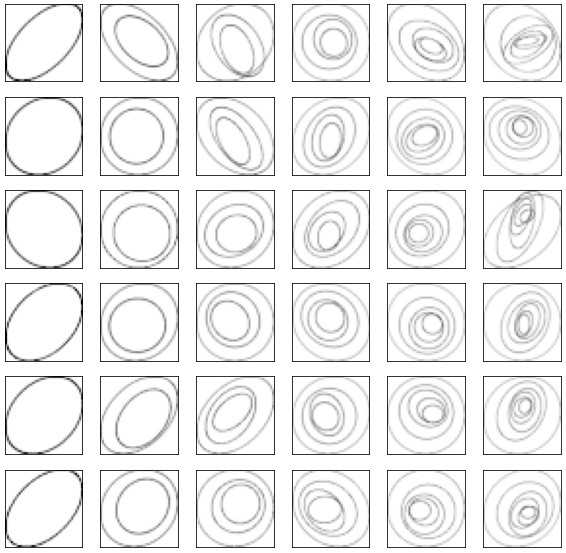
\includegraphics[width=0.5\textwidth]{nested_ellipses.PNG}
    \caption{Sample of the artificial nested ellipses datasets. First column is taken from the first dataset with 1 ellipse, second columns from the second dataset with 2 nested ellipses, until the sixth column with 6 nested ellipses.}
\end{figure}

\begin{table}[h] \label{table1}
  \centering
  \caption{Mean density with the number of nested ellipses. The density has been calculated by averaging the ratio of non-null pixel per images over 100 generated pictures for each dataset sharing the same number $n_{ellipses}$ of nested ellipses.}
  \renewcommand{\arraystretch}{1.5} % Modify the row height
  \begin{tabular}{|c|c|c|c|c|c|c|}
    \hline
    $n_{ellipses}$ & 1 & 2 & 3 & 4 & 5 & 6 \\
    \hline
    $Density$ ($\%$) & 29.0 & 51.4 & 64.3 & 70.9 & 73.5 & 75.0 \\
    \hline
  \end{tabular}
\end{table}


% Note that in this section, we study the time performance of the algorithm with no concern about convergence nor convergence speed, therefore MAM has not been fully optimized in term of convergence: $\rho$ has been set to 100 for every datasets.
% %, as this seems to be a mean value of the optimized hyperparameter. 
% No further refinement have been conducted. 
In this first experiments we analyze the impact over MAM caused by the sparsity and number of measures. We have set $\rho=100$ without proper tuning for every dataset. The study has been carried out with one processor to avoid CPU communication management.\\


% graphs of the results
\begin{figure} \label{surface}
    \centering
    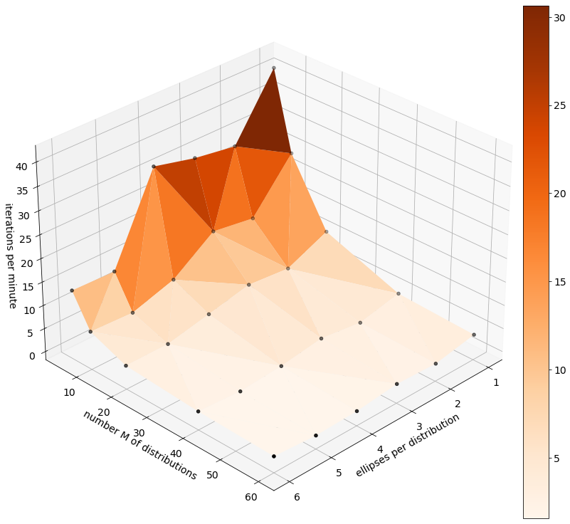
\includegraphics[width=0.8\textwidth]{surface_influence_parameters.png}
    \caption{Evolution of the number of iterations per minute depending on the density or the number of distributions.}
\end{figure}

\cref{surface} shows that, as expected, the execution time of an iteration increases with increasing density and number of measures.
% But decay rate is stronger with the dependency of the number of ellipses per distribution, it induces 
When compared to density it can be seen that the number of measures has greater influence on the method's speed (such a phenomenon can be due to the $numpy$ matrix management). 
%This can be explained by the fact that \textit{Step 2} is computed using $numpy$ that parallelize the vectorized projections of the columns of each marginal matrices before iterating to the next distribution matrice (in the \textit{for loop}). Therefore this result can be slightly different if another way of coding is taken into account, but such a way would be less efficient : $Matlab$ or $C$ can also take advantage of this intern parallelizable algebric step with vectorized matrices. [REFERENCE CODE PYTHON GITHUB ?] \\
% We underline that the number of distribution treated has an expected impact on the computation performances while the density of the support has little impact. 
This means the quantity of information in each measure does not seem to make the algorithm less efficient in term of speed. Such a result is to be put in regard with algorithms such as B-ADMM \cite{J.Ye} that are particularly shaped for sparse dataset but less efficient for denser ones.  This is a significant point that will be further developed in \cref{infl_support}.\\


\subsection{Comparison with IBP}
The Iterative Bregman Projection (IBP) \cite{IBP} is a state-of-the-art algorithm for computing Wasserstein barycenters. As mentionned in the Introduction, IBP employes a regularizing function parametrized by $\lambda>0$.
% IBP 
% %is based on an entropic regularization of the problem, and 
% can be rephrased into a two step iterative algorithms, where one step is the free-space move in the dual space, and the other is the Bregman projection in the primal space. The main idea, to make this iterative algorithm a reformulation of the initial problem, is in fact to transform the problem thanks to a penalization tuned with an hyperparameter $\lambda$, making IBP an inexact approach (see \cref{introduction}). 
The greater the $\lambda$, the worst the approximation. But in practice, $\lambda$ has to be kept in a moderate magnitude to avoid numerical errors (double-precision overflow). IBP is very sensitive to $\lambda$, that strongly relies on the dataset at stake. Thus IBP is an inexact method, whereas MAM is exact. Although the study below shows certain advantages of MAM, we make it clear that the aim is not to demonstrate which algorithm is better in general but instead to highlight the differences between the two methods and their advantages depending on the use. Note that the code for IBP is inspired from the original \cite{IBP_github}.

\subsubsection{Qualitative comparison} \label{qualitative_sec}
Here we use 100 images per digit of the MNIST database \cite{MNIST_database} where each digit has been randomly translated and rotated. Each image has 40 $\times$ 40 pixels and can be treated as probability distributions thanks to a normalization, where the pixel location is the \textit{support} and the pixel intensity the \textit{probability}. In \cref{barycenter_evolution}, we display intermediate barycenter solutions for digits $3, 4, 5$ at different time steps both for MAM and IBP. For the two methods the hyperparameters have been tuned: 
%. In the case of IBP, the larger is $\lambda$ the closer is the obtained solution to the exact solution \cite{J.Ye}
for instance, $\lambda = 1700$ is the greatest lambda that enables IBP to compute the barycenter of the 3's dataset without double-precison overflow error. Regarding MAM, a range of values for $\rho>0$ have been tested for 100 seconds of execution, to identify which one provides good performance (for example, $\rho=50$ for the dataset  of $3$'s).

% graphs of the results
\begin{figure}[h!] \label{barycenter_evolution}
    \centering
    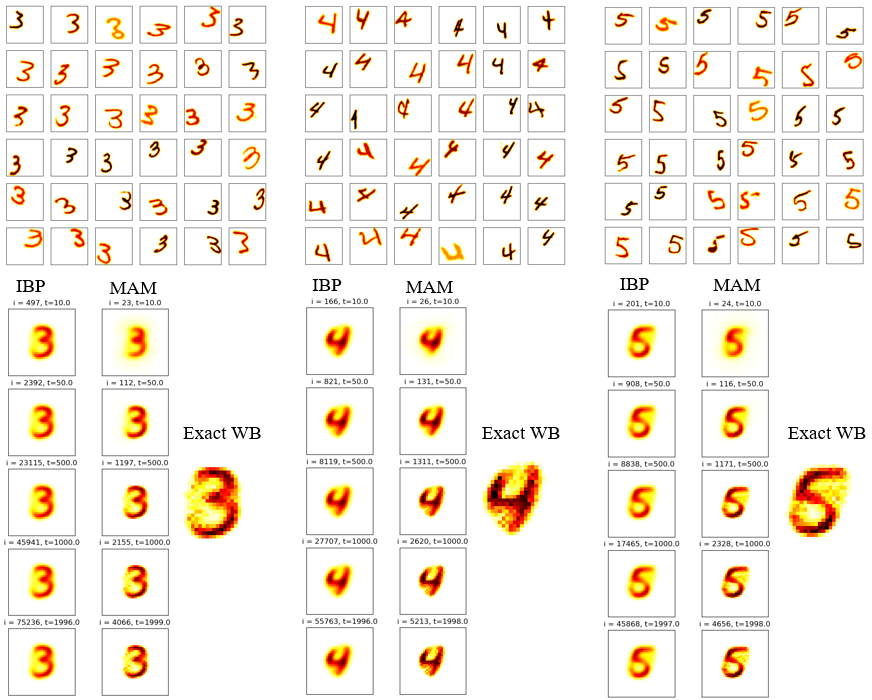
\includegraphics[width=1\textwidth]{qualitative_345.png}
    \caption{(top) For each digit 36 out of the 100 scaled, translated and rotated images considered for each barycenter. (bottom) Barycenters after $t = 10, 50, 500, 1000, 2000$ seconds, where the left-hand-side is IBP evolution of its barycenter approximation, the middle panel is MAM evolutions using 10 CPU
    and the right-hand-side is the exact solution computed by applying \textit{Gurobi} to the LP \cref{HugeLP}.}
\end{figure}

As illustrated in \cref{barycenter_evolution}, for each dataset, IBP gets quickly to a stable approximation of a barycenter. Such a point is obtained shortly after with MAM (less than 5 to 10 seconds after) but MAM continues to converge toward a sharper solution (closer to the exact solution as exemplified quantitatively in \cref{quantitative_section}). It is clear that the more CPUs used for MAM the better. We have limited the study to a dozen of CPU to allow the reader to reproduce the experimentations. While IBP is not well shaped for CPU parallelization  \cite{IBP_github, IBP, J.Ye}, MAM offers a clear advantage depending on the hardware at stake.


\subsubsection{Quantitative comparison} \label{quantitative_section}
Next we benchmark MAM, randomized MAM and IBP on a dataset with 60 images per digit of the MNIST database \cite{MNIST_database} where every digit is a normalized image 40 $\times$ 40 pixels. 
% This corresponds to a limit to compute the exact solution with a Linear Program (LP) with 150Gb RAM [INFORMATION CORRECT ON THE DIGITAL SANDBOX?? cf lscpu], using \textit{scipy.optimize.linprog} on \textit{python}.
First, all three methods have their hyperparameters tuned thanks to a sensitivity study as explained in \cref{qualitative_sec}. Then, at every time step an approximation of the computed barycenter is stored, to compute the error $\bar W_2^2(p^{k}) -\bar W_2^2(p_{exact}) := \sum_{m=1}^M \frac{1}{M}{\tt OT}(p^k,q^{(m)}) - \sum_{m=1}^M \frac{1}{M}{\tt OT}(p_{exact},q^{(m)})$.
% % The distances  $W_2^2(\mu^{(k)}, \nu^{(m)})$ between the intermediate barycenter and the distributions at stakes are calculated thanks to an LP and uniformly averaged to get the exact barycentric distance defined as $\bar W_2^2(\mu^{k}) := \frac{1}{M} \sum_{m=0}^M W_2^2(\mu^k, \nu^{(m)})$.
% The Linear Program to compute the exact value of \cref{ordonnee} uses the HIGHS method \cite{huangfu2018parallelizing} implemented with \textit{scipy} in \textit{python}. The resolution for $M=60$ exploited the total memory of our computer, thus imposing serious limitations on the number of measures that can be dealt with and if one aim at higher dimensions, computing the barycenter via an LP is out of reach \footnote{\textit{Gurobi} can be used to push the limit a bit as exemplified in \cref{qualitative_sec}.}.\\
All methods were implemented in $python$ using a \textit{MPI} based parallelization. Note that IBP is inspired from the code of G. Peyré \cite{IBP_github}, MAM from \cref{alg} and MAM-randomized (\cref{rem:random}) has only one distribution treated by processor. 
%The influence of the number of processors is studied by carrying out computations with varying numbers of processors.
%computations with varying number of processors
% The influence of the number of processors is studied using CPU.
\cref{IBP_vs_MAM} displays the evolution w.r.t time, of the error measure $\bar W_2^2(p^{k}) -\bar W_2^2(p_{exact})$, with $p_{exact}$ an exact barycenter obtained by solving LP \cref{HugeLP} directly.


% graphs of the results
\begin{figure}[h!] \label{IBP_vs_MAM}
    \centering
    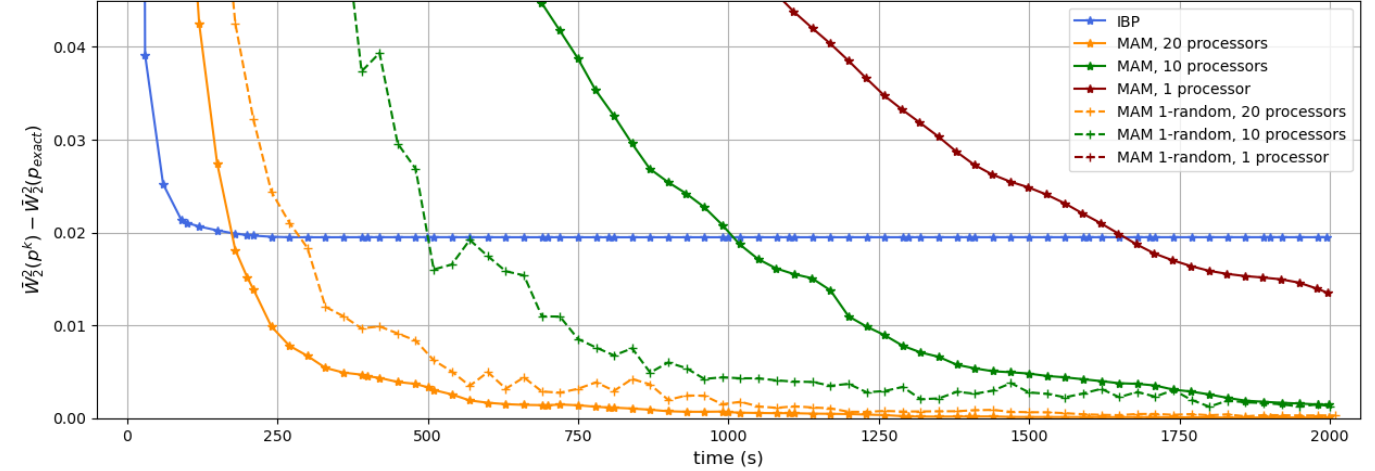
\includegraphics[width=1\textwidth]{IBP_vs_MAM.png}
    \caption{Evolution with respect to time of the difference between the Wasserstein barycenter distance of an approximation, $\bar W_2^2(p^{k})$, and the Wasserstein barycentric distance of the exact solution $\bar W_2^2(p_{exact})$ given by the LP. The time step between two points is 30 seconds.}
\end{figure}

It is clear that IBP is almost 10 time faster per iteration.
%, but being faster in one iteration does not mean faster speed overall.
However IBP computes an exact solution of an approximated problem that is tuned through the hyperparameter $\lambda$ (see \cite{IBP}). Therefore it is natural to witness IBP converging to a solution to the approximated problem, but not to an exact WB. While MAM does converge to an exact solution. So there is a threshold where the accuracy of MAM exceeds IBP: in our case, around 200s - for the computation with the greatest number of processors (see \cref{IBP_vs_MAM}).
% As expected, the more processors, the quicker the algorithm converges to a solution. Note that for every number of processors, the method converge to the same solution. Therefore the threshold where MAM becomes more accurate than IBP 
Such a treshold always exists depending on the computational means (hardware).\\
This quantitative study explains what have been exemplified with the images of \cref{qualitative_sec}: the accuracy of IBP is bounded by the choice of $\lambda$, itself bounded by an overflow error, while MAM hyperparameters only impact the convergence speed and the algorithm is always improving towards an exact solution. For this dataset, the WB computed by IBP is within 2$\%$ of accuracy and thus reasonably good. However, as shown in Table 1 in \cite{J.Ye}, one can choose other datasets where IBP's accuracy might be unsatisfactory.\\
% : \wlo{Table I in \cite{J.Ye} shows errors of approximately 20$\%$, while for such a dataset, MAM has the same behavior than exemplified above and quickly reaches an accurate solution (\cref{BADMM_vs_MAM} elaborates more precisely about MAM performances on this dataset).} \\
\\
Furthermore, \cref{IBP_vs_MAM} exemplifies an interesting asset of randomized variants of MAM: for some configurations randomized-MAM is more efficient than (deterministic) MAM but for others, the latter seems to be more effective.
Note that the curve \textit{MAM 1-random, 1 processor} does not appear on the figure: this is because it is above the y-axis value range due to its bad performance.
Indeed, there is a trade-off between time spent per iteration and precision gained after an iteration. For example, with 10 processors, each processor treats 6 measures in the deterministic MAM but only one is treated in the randomized MAM. Therefore, the time spent per iteration is roughly six time shorter in the latter and this counterbalances the loss of accuracy per iterations. On the other hand, when using 20 processors, only 3 measures are treated by each processor and the trade-off is not worth it anymore: the gain in time does not compensate for the loss in accuracy per iteration. One should adapt the use of the algorithm with care since this trade-off conclusion is only heuristic and strongly depends on the dataset and hardware at use. A sensitivity analysis is always a good thought for choosing the most effective amount of measures handled per processor while using the randomized-MAM against the deterministic MAM.

\subsubsection{Influence of the support} \label{infl_support}
This section is echoing \cref{parametric_section} and studies the influence of the support size. To do so, two datasets have been tested for MAM and IBP. The first dataset is already used in \cref{quantitative_section}: 60 pictures of 3's taken from the classic MNIST database \cite{MNIST_database}. The second dataset is also composed by these 60 images but each digit has been randomly translated and rotated in the same way as in \cref{barycenter_evolution}. Therefore, the union of the support of the second dataset is greater than the first one, as illustrated in \cref{fig_support}.

\begin{figure}[h] \label{fig_support}
    \centering
    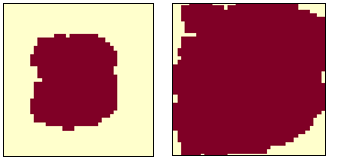
\includegraphics[width=0.5\textwidth]{support_datasets.png}
    \caption{Images with $40 \times 40$ pixel grid, where the red represents the pixels which are in the union of the dataset support composed with 60 images. (left) for the standard MNIST, (right) for the randomly translated and rotated MNIST.}
\end{figure}

\cref{fig_compare_support} presents two graphs that have been obtained just as in \cref{quantitative_section}, but displaying the evolution w.r.t time in percentage: $\Delta W_{\%} := \frac{\bar W_2^2(p^{k}) -\bar W_2^2(p_{exact}) }{\bar W_2^2(p_{exact})} \times 100$. Once more, the hyperparameters have been fully tuned. The hyperparameter of the IBP method is smaller for the second datacase. Indeed, as stated in \cite{J.Ye}, the greater is the support, the stronger are the restrictions on $\lambda$. And since the smaller is $\lambda$ the further is the approximated problem to the exact one this is expected to witness rising differences between on the following graphs. 
%As suggested in \cite{J.Ye}, this numerical difficulty can be partly addressed by treshholding entries that are too small and active research is carried in this direction but won't be deepen here.\\


% results
\begin{figure}[h] \label{fig_compare_support}
    \centering
    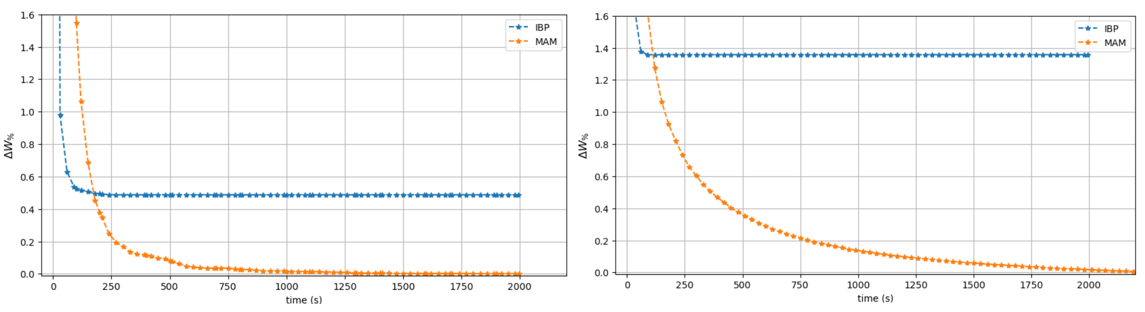
\includegraphics[width=1\textwidth]{IBP_vs_MAM_support_pourcentage.png}
    \caption{Evolution of the percentage of the distance between the exact solution of the barycenter problem and the computed solution using IBP and MAM method with 20 processors: (left) for the standard MNIST, (right) for the randomly translated and rotated MNIST. %\wlo{Ce graphique a des ordonnées en pourcentages pour comparer : c'est logique. Le graph d'au dessus à des ordonnées en valeurs absolu pour 'cacher' les faibles pourcentages, qu'en pensez vous ? Je devrais peut être tout mettre en pourcentage non?} 
    }
\end{figure}

Being an exact method, MAM is insensitive to support size. The density of the dataset has little impact on the convergence time as explained in \cref{parametric_section} and exemplified in \cref{fig_compare_support}. 
%IBP does not converge to the exact solution and because of the hyperparameter limitation, the larger is the support and the farther is the converged approximation. This is critical in the second case scenario where the approximation is almost four time farther than with the first dataset, while the support at stake is only three times larger. 
Such visual results concerning IBP initialization and parametrization have already been discussed in \cref{barycenter_evolution}, some other qualitative results can be found in \cite{Puccetti} where the author shows that properties of the distributions can be lost due to the entropy penalization in IBP.

\subsection{Comparison with B-ADMM} \label{BADMM_vs_MAM}
This subsection compares MAM with the algorithm B-ADMM of \cite{B-ADMM} using the dataset and Matlab implementation provided by the authors at the link \url{https://github.com/bobye/d2_kmeans}. We omit  IBP in our analysis because it has already been shown in  \cite[Table I]{B-ADMM} that IBP is outperformed by B-ADMM in this dataset. As in \cite[Section IV]{B-ADMM}, we consider $M=1000$ discrete measures, each with a sparse finite support set obtained by clustering pixel colors of images.
The average number of support points is around $6$, and the barycenter's number of (fixed) support points is $R=60$.
An exact WB can be computed by applying an LP solver to the extensive formulation \cref{HugeLP}. Its optimal value is $712.7$, computed in $10.6$ seconds by the Gurobi LP solver. We have coded MAM in Matlab to have a fair comparison with the Matlab B-ADMM algorithm provided at the above link. Since MAM and  B-ADMM use different stopping tests, we have set their stopping tolerances equal to zero and let the solvers stop with a maximum number of iterations. \Cref{tab:MAMxBADMM} below reports CPU time in seconds and the objective values yielded by the (approximated) barycenter $\tilde p$ computed by both solvers: $\bar W_2^2(\tilde p)$.
\begin{table}[htb]
\centering
  \caption{MAM vs B-ADMM. The considered implementation of B-ADMM is the one provided by its designers without changing parameters (except the stopping set to zero and the maximum number of iterations). Both algorithms use the same initial point. The dataset is the one considered in \cite[Section IV]{B-ADMM}. The optimal value of the WB barycenter for this dataset is $712.7$, computed by Gurobi in $10.6$ seconds. }
  \label{tab:MAMxBADMM}
\begin{tabular}{|c|cc|cc|}
\hline
\multirow{2}{*}{Iterations} & \multicolumn{2}{c|}{Objective value} & \multicolumn{2}{c|}{Seconds}       \\ \cline{2-5} 
                            & \multicolumn{1}{c|}{B-ADMM}  & MAM   & \multicolumn{1}{c|}{B-ADMM} & MAM  \\ \hline
100                         & \multicolumn{1}{c|}{742.8}   & 716.7 & \multicolumn{1}{c|}{1.1}    & 1.1  \\ \hline
200                         & \multicolumn{1}{c|}{725.9}   & 714.1 & \multicolumn{1}{c|}{2.4}    & 2.2  \\ \hline
500                         & \multicolumn{1}{c|}{716.5}   & 713.3 & \multicolumn{1}{c|}{5.6}    & 5.4  \\ \hline
1000                        & \multicolumn{1}{c|}{714.1}   & 712.9 & \multicolumn{1}{c|}{11.8}   & 10.8 \\ \hline
1500                        & \multicolumn{1}{c|}{713.5}   & 712.8 & \multicolumn{1}{c|}{18.9}   & 16.2 \\ \hline
2000                        & \multicolumn{1}{c|}{713.3}   & 712.8 & \multicolumn{1}{c|}{25.1}   & 21.6 \\ \hline
2500                        & \multicolumn{1}{c|}{713.2}   & 712.8 & \multicolumn{1}{c|}{31.0}   & 27.1 \\ \hline
3000                        & \multicolumn{1}{c|}{713.1}   & 712.7 & \multicolumn{1}{c|}{39.8}   & 32.4 \\ \hline
\end{tabular}
\end{table}


The results show that, for the considered dataset, MAM and B-ADMM are comparable regarding CPU time, with MAM providing more precise results. In contrast with MAM, B-ADMM does not have (at this time) a convergence analysis. 

\if{ % following results are not worht presenting...

\Cref{tab:MAM-random} compares MAM with three random variants in a serial environment with only one processor. To this end, we have fixed the CPU time for the random variants to the values of \cref{tab:MAMxBADMM}: the first column in \cref{tab:MAM-random} is the last one in \cref{tab:MAMxBADMM}, and the last column in \cref{tab:MAMxBADMM} is the third one in \cref{tab:MAMxBADMM}.
For instance, solver MAM-50 is the random variant of \cref{alg} with $50$ measures randomly chosen at every iteration.




\begin{table}[htb]
\centering
  \caption{Comparison of MAM (deterministic) and three randomized variants on the dataset of \cite{B-ADMM}. }
  \label{tab:MAM-random}
\begin{tabular}{|c|ccccl|}
\hline
\multirow{2}{*}{Seconds} & \multicolumn{5}{c|}{Objective value}                                                                                                                \\ \cline{2-6} 
                         & \multicolumn{1}{c|}{MAM-5} & \multicolumn{1}{c|}{MAM-50} & \multicolumn{1}{c|}{MAM-100} & \multicolumn{1}{c|}{MAM-500} & MAM                        \\ \hline
1.1                      & \multicolumn{1}{c|}{723.2} & \multicolumn{1}{c|}{716.9} & \multicolumn{1}{c|}{716.5}   & \multicolumn{1}{c|}{716.6}   & 716.7                      \\ \hline
2.2                      & \multicolumn{1}{c|}{716.4} & \multicolumn{1}{c|}{713.9}  & \multicolumn{1}{c|}{714.4}   & \multicolumn{1}{c|}{714.1}   & 714.1                      \\ \hline
5.4                      & \multicolumn{1}{c|}{714.0} & \multicolumn{1}{c|}{713.3}  & \multicolumn{1}{c|}{713.3}   & \multicolumn{1}{c|}{713.2}   & 713.3                      \\ \hline
10.8                     & \multicolumn{1}{c|}{713.3} & \multicolumn{1}{c|}{712.9}  & \multicolumn{1}{c|}{712.9}   & \multicolumn{1}{c|}{712.9}   & 712.9                      \\ \hline
16.2                     & \multicolumn{1}{c|}{713.0} & \multicolumn{1}{c|}{712.8}  & \multicolumn{1}{c|}{712.9}   & \multicolumn{1}{c|}{712.8}   & \multicolumn{1}{c|}{712.8} \\ \hline
21.2                     & \multicolumn{1}{c|}{713.0} & \multicolumn{1}{c|}{712.8}  & \multicolumn{1}{c|}{712.8}   & \multicolumn{1}{c|}{712.8}   & \multicolumn{1}{c|}{712.8} \\ \hline
27.1                     & \multicolumn{1}{c|}{712.9} & \multicolumn{1}{c|}{712.8}  & \multicolumn{1}{c|}{712.8}   & \multicolumn{1}{c|}{712.8}   & \multicolumn{1}{c|}{712.8} \\ \hline
32.4                     & \multicolumn{1}{c|}{712.8} & \multicolumn{1}{c|}{712.8}  & \multicolumn{1}{c|}{712.7}   & \multicolumn{1}{c|}{712.7}   & \multicolumn{1}{c|}{712.7} \\ \hline
\end{tabular}
\end{table}
In same cases, the randomized variant performs slightly better. For instance, the variants MAM-50 and MAM-100 manage to reach the optimal value faster than the deterministic variant: see the penultimate line in \cref{tab:MAM-random}. 
}\fi

\subsection{Unbalanced Wasserstein Barycenter} \label{sec:resul-UWB}
% \wlo{Est-il necessaire de motivier une fois de plus le cas unbalanced, peut être que j'en dis trop, je voulais motiver dans le cadre applicatif ?}
% It is possible to normalize images, such as by subtracting the mean and dividing by the standard deviation (we only divide by the sum of  the pixels values in our studies), to obtain images with similar statistical properties. However, in some cases, it may not be appropriate to normalize the images or it may not be sufficient to obtain images that are visually similar. \\
% For example, consider a set of images that have different levels of contrast or brightness. Normalizing these images may not be sufficient to make them visually similar, as the differences in contrast and brightness will still be present in the normalized images. In this case, the UWB can be used to compute a barycenter image that represents the set of images, taking into account the differences in contrast and brightness. \\
% Furthermore, the UWB can be used to generate new images that are representative of the set, but with specific characteristics. For example, one can compute the UWB of a set of blurred images with different levels of blur, and then generate new images with a specific level of blur by interpolating between the blurred images and the UWB. This can be useful in applications such as deblurring or image restoration. \\
% Overall, while normalizing images can be effective in some cases, the UWB provides a more general framework for computing representative images of a set with varying characteristics.
% \\

This section treats a particular example to illustrate the interest of using UWB. The artificial dataset is composed by 50 images with resolution $80\times80$. Each image is divided in four squared. The top left, bottom left and bottom right squared are randomly filled with double nested ellipses and the top right squared is always empty as exemplified in \cref{dataset_unbalanced}. In this example, every image is normalized to depict a probability measure so that we can compare WB and UWB.

\begin{figure}[h] \label{dataset_unbalanced}
    \centering
    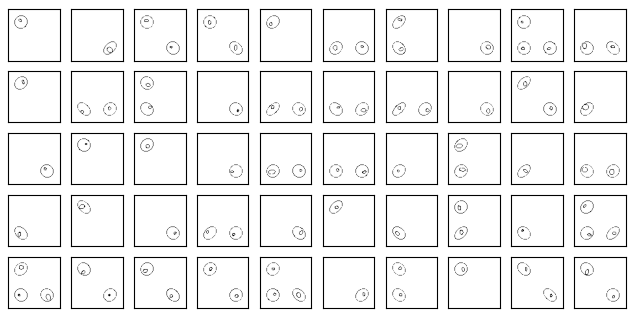
\includegraphics[width=.8\textwidth]{dataset_unbalanced_2_50pics.png}
    \caption{Dataset composed by 50 pictures with nested ellipses randomly positionned in the top left, bottom right and left corners.}
\end{figure}

With respect to \cref{UWB}, one set of constraints is relaxed and the influence of the hyperparameter $\gamma$ is studied. If $\gamma$ is large enough (i.e. greater than $\norm{{\tt vec}(d)} \approx 1000$, see \cref{prop_gamma}), the problem boils down to the standard WB problem since the example deals with probability measures: the resulting UWB is indeed a WB.  When decreasing $\gamma$ the transportation costs take more importance than the distance to $\L$ that is more and more relaxed. Therefore, as illustrated by \cref{res_gamma}, the resulting UWB splits the image in four parts, giving visual meaning to the barycenter.

\begin{figure}[h] \label{res_gamma}
    \centering
    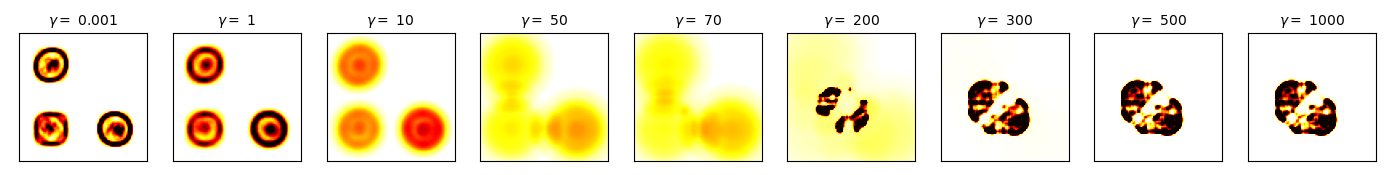
\includegraphics[width=1.\textwidth]{UWB_gamma_M50.PNG}
    \caption{UWB computed with MAM for different values of $\gamma$.}
\end{figure}


% [NOT IN THE ARTICLE]
% \cref{sec:ext} introduces the more generalized UWB problem that relaxes the constraints on $p$ and on $q^{(m)}, m=1...M$. \cref{res_eta} analyzes the impact of the newly introduced hyperparameter $\eta$ which tunes the penalization of the left constraints, while the right constraints are kept ($\gamma$ is set to a large value). Expected results are obtained: with $\eta$ tending to $0$, the transformed LP has no constraint linking $q^{(m)}$ and $\pi^{(m)} \textit{, for all } m=1...M$, therefore a straightforward solution is $\pi^{(m)}_{rs} = 0, r=1...R, s=1...S^{(m)}, m=1...M$. On the other hand, when $\eta$ is large the penalization on the left constraints is important and the UWB problem tends to the WB problem.\\
% The intermediate solutions have the same support than the WB but with reduced weights. In fact the transported distributions are no longer bounded to be the $q^{(m)}, m=1...M$, when reducing $\eta$ the transported distributions are images with support like the initial distributions but with reduced weights.

% \begin{figure}[h] \label{res_eta}
%     \centering
%     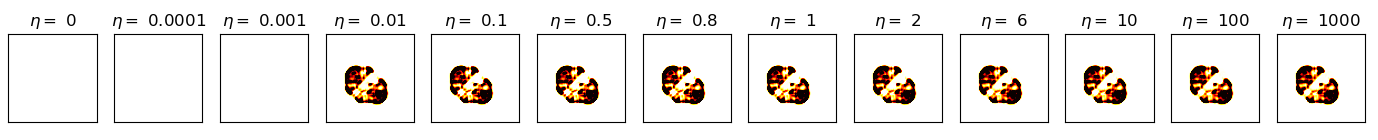
\includegraphics[width=1.\textwidth]{UWB_eta.PNG}
%     \caption{UWB computed with MAM for different hyperparameter $\gamma$.}
% \end{figure}

% \cref{res_eta_gamma} illustrates the influence of the parameters $\gamma$ and $\eta$, they must be tuned depending on the wanted behavior of the UWB. [PLUS D'EXPLICATIONS ?]

% \begin{figure}[h] \label{res_eta_gamma}
%     \centering
%     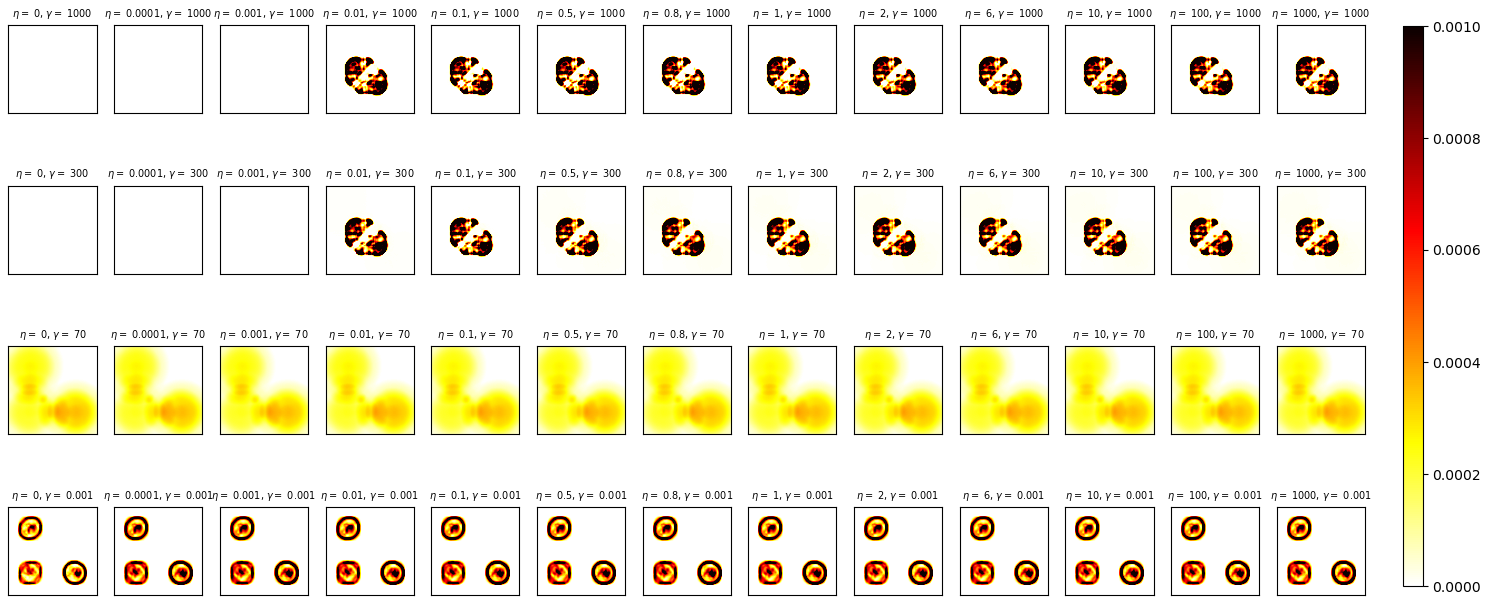
\includegraphics[width=1.\textwidth]{evolution_gamma_eta.PNG}
%     \caption{UWB computed with MAM for different hyperparameter $\gamma$.}
% \end{figure}

In the same vein, \cref{UWB_ill_MAM} provides an illustrative application of MAM for computing UWB in another dataset.

\begin{figure}[h] \label{UWB_ill_MAM}
    \centering
    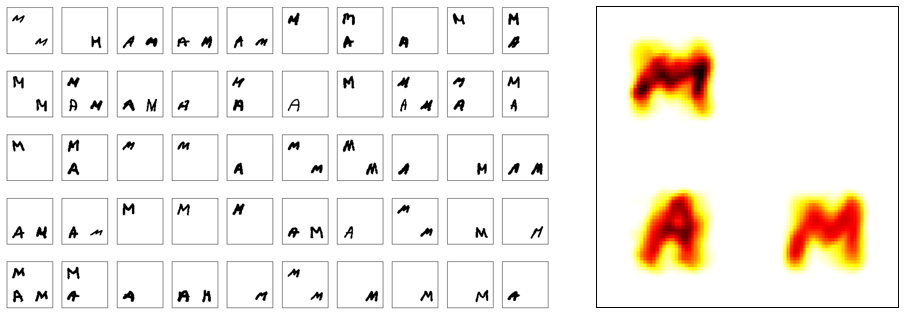
\includegraphics[width=1.\textwidth]{UWB_MAM_ill.PNG}
    \caption{\textit{(left)} UWB for a dataset of letters M-A-M built in the same logic than \cref{dataset_unbalanced} with 50 figures: \textit{(right)} resulting UWB with $\gamma=0.01$, computed in 200 seconds using 10 processors.} %en vérité 1000s mais au bout de 200 secondes on a deja ce résultat visuel
\end{figure}



% \newpage
%\section{Conclusion}

% In this study, we have presented a novel approach for computing the Wasserstein barycenter of discrete measures, leveraging the Douglas-Rachford theory. Through this innovative methodology, we have achieved convergence to the exact Wasserstein barycenter, and convergence proofs have been established based on the DR theory. \\
% Moreover, we have extended our proposed method to address the unbalanced case, resulting in the formulation of the unbalanced Wasserstein barycenter. We have introduced a new formulation of the UWB problem that relaxes only one side of the constraints, and we have further extended this definition to encompass the general case where both sides are relaxed.\\
% To assess the effectiveness of our algorithm, we conducted comprehensive comparisons against state-of-the-art methods such as IBP and B-ADMM. The results of these experiments highlighted the efficiency of MAM, which consistently converges to the exact Wasserstein barycenter. While we acknowledge that depending on the need, IBP can exhibits superior performance, these findings still support the efficacy and competitiveness of our approach.\\
% Furthermore, we have demonstrated the versatility and applicability of MAM by successfully applying it to the broader UWB problem.
% + limites


\newpage

\bibliographystyle{plain}
\bibliography{references}

\newpage
\appendix

%%%%%%%%%COMMENTED%%%%%%%%%%%%
\if{
\section{Proof of ~\cref{prop_2}} \label{prof_step_1}
%\begin{proof}
First, observe that $\pi^{k+1}={\tt Proj}_{\L}(\theta^k)$ solves the QP problem
\[
\left\{
\begin{array}{llllllll}
\displaystyle \min_{\pi^{(1)},\ldots,\pi^{(M)}} & \displaystyle \frac{1}{2} \sum_{m=1}^M \norm{\pi^{(m)}- \theta^{(m),k}}^2\\
\mbox{s.t} &  \sum_{s=1}^{S^{(1)}} \pi^{(1)}_{rs} &= \sum_{s=1}^{S^{(2)}} \pi^{(2)}_{rs},&\; r=1,\ldots,R\\
&\sum_{s=1}^{S^{(2)}} \pi^{(2)}_{rs} & = \sum_{s=1}^{S^{(3)}} \pi^{(3)}_{rs},&\; r=1,\ldots,R\\
&&\vdots\\
&\sum_{s=1}^{S^{(M-1)}} \pi^{(M-1)}_{rs} &= \sum_{s=1}^{S^{(M)}} \pi^{(M)}_{rs},&\; r=1,\ldots,R
\end{array}
\right.
\]
Note that this problem is only coupled 
by the ``columns" of $\pi$: there is no constraint liking $\pi^{(m)}_{rs}$ with $\pi^{(m')}_{r's}$ for $r\neq r'$ and $m$ and $m'$ arbitrary. Therefore, we can decompose it by rows: for $r=1,\ldots,R$, the $r^{th}$-row 
\[(\pi^{(1),k+1}_{r1},\ldots,\pi^{(1),k+1}_{rS^{(1)}},\ldots,\pi^{(M),k+1}_{r1},\ldots,\pi^{(M),k+1}_{rS^{(M)}})\] of $\pi^{k+1}$ is the unique solution of
\begin{equation}\label{eq:proj_row}
\left\{
\begin{array}{llllllll}
\displaystyle \min_{\pi^{(1)}_{r1},\ldots,\pi^{(M)}_{rS^{(M)}}} & \displaystyle \frac{1}{2} \sum_{m=1}^M
\sum_{s=1}^{S^{(m)}} \Big(\pi^{(m)}_{rs} - \theta^{(m),k+1}_{rs}\Big)^2\\
\mbox{s.t} &  \sum_{s=1}^{S^{(1)}} \pi^{(1)}_{rs} &= \sum_{s=1}^{S^{(2)}} \pi^{(2)}_{rs}\\
&\sum_{s=1}^{S^{(2)}} \pi^{(2)}_{rs} & = \sum_{s=1}^{S^{(3)}} \pi^{(3)}_{rs}\\
&&\vdots\\
&\sum_{s=1}^{S^{(M-1)}} \pi^{(M-1)}_{rs} &= \sum_{s=1}^{S^{(M)}} \pi^{(M)}_{rs}.
\end{array}
\right.
\end{equation}
In the following developments we denote the $r^{th}$ row of $\pi$ and $\theta^{k}$ by $\pi_{r:}$ and $\theta^{k}_{r:}$ (in $\mathbb{R}^{\sum_{m=1}^M S^{(m)}}$), respectively. The (column) vector of ones in $\mathbb{R}^{S^{(m)}}$ is represented by $\mathbf{1}_{S^{(m)}}$. Accordingly, the above problem boils down to
\begin{equation}\label{eq:proj_row_w}
\left\{
\begin{array}{llllllll}
\displaystyle \min_{\pi^{(1)}_{r:},\ldots,\pi^{(S)}_{r:}} & \displaystyle \sum_{m=1}^M\frac{1}{2} 
\norm{\pi^{(m)}_{r:} - \theta^{(m),k}_{r:}}^2\\
\mbox{s.t} &  \pi^{(1)}_{r:}\mathbf{1}_{S^{(1)}} &=  \pi^{(2)}_{r:} \mathbf{1}_{S^{(2)}}&\qquad(u^{(1)})\\
&\pi^{(2)}_{r:}\mathbf{1}_{S^{(2)}} & = \pi^{(3)}_{r:}\mathbf{1}_{S^{(3)}}&\qquad(u^{(2)})\\
&&\vdots\\
&\pi^{(M-1)}_{r:}\mathbf{1}_{S^{(M-1)}} &= \pi^{(M)}_{r:} \mathbf{1}_{S^{(M)}}&\qquad(u^{(S-1)}).
\end{array}
\right.
\end{equation}
The dual variables associated to every constraint above are given between parenthesis.
The Lagrangian function to this problem is, for a dual variable $u$, given by
\[
L(\pi_{r:},u)= \displaystyle \sum_{m=1}^M\frac{1}{2} 
\norm{\pi^{(m)}_{r:} - \theta^{(m),k}_{r:}}^2
+  \sum_{m=1}^{M-1} u^{(m)}\Big( \pi^{(m)}_{r:}\mathbf{1}_{S^{(m)}} -  \pi^{(m+1)}_{r:}\mathbf{1}_{S^{(m+1)}}\Big).
\]
A solution to problem~\cref{eq:proj_row_w} must satisfy $\nabla_{\pi{_r:}} L(\pi^{k+1}_{_r:},u)=0$, that is,
\begin{equation}\label{eq:sytemL}
\begin{pmatrix}
\pi_{r:}^{(1),k+1}- \theta_{r:}^{(1),k} \\
\pi_{r:}^{(2),k+1}- \theta_{r:}^{(2),k} \\
\pi_{r:}^{(3),k+1}- \theta_{r:}^{(3),k}\\
\vdots \\
\pi_{r:}^{(M-1,k+1)}- \theta_{r:}^{(M-1),k}\\
\pi_{r:}^{(M),k+1}- \theta_{r:}^{(M),k}\\
\end{pmatrix}
+
\begin{pmatrix}
u^{(1)}\mathbf{1}_{S^{(1)}} \\
u^{(2)}\mathbf{1}_{S^{(2)}}- u^{(1)}\mathbf{1}_{S^{(2)}}\\
u^{(3)}\mathbf{1}_{S^{(3)}}- u^{(2)}\mathbf{1}_{S^{(3)}}\\
\vdots \\
u^{(M-1)}\mathbf{1}_{S^{(M-1)}}- u^{(M-2)}\mathbf{1}_{S^{(M-1)}}\\
- u^{(M-1)}\mathbf{1}_{S^{(M)}}
\end{pmatrix}
=0.
\end{equation}
%We claim that $p_r= \pi^{(1)}_{r:}\mathbf{1}_{S^{(1)}}$ ($=\pi^{(m)}_{r:}\mathbf{1}_{S^{(m)}}$ for all $m$ due to feasibility of $\pi_{r:}$) is given by
%\[
%p_r= \frac{\sum_{m=1}^M \frac{\sum_{s=1}^{S^{(m)}}\theta_{rs}^{(m),k}}{ S^{(m)}} }{\sum_{m=1}^M \frac{1}{S^{(m)}}}.
%\]
%(The proof of this result does not follow from the above Lagrange system, by from the one written for the constraints $\mathbf{1}_{N^{(s)}}^\top w^{(s)}=p_m$, $s=1,\ldots,S$.)
Let us denote $p_r^k= \pi^{(1),k+1}_{r:}\mathbf{1}_{S^{(1)}}$ ($=\pi^{(m),k+1}_{r:}\mathbf{1}_{S^{(m)}}$ for all $m$ due to feasibility of $\pi_{r:}$)
%. Having determined $p_m$, the dual variables in the above system can be obtained recursively. To this end, lets 
and multiply the first set of equations by $\mathbf{1}_{S^{(1)}}$ to get 
\[
p_r^k- \theta^{(1),k}_{r:}\mathbf{1}_{S^{(1)}}
 + u^{(1)}{S^{(1)}} = 0\quad \Rightarrow \quad u^{(1)}:= \frac{ \theta^{(1),k}_{r:}\mathbf{1}_{S^{(1)}}-p_r^k}{S^{(1)}}=\frac{ \sum_{s}^{S^{(1)}}\theta^{(1),k}_{rs}-p_r^k}{S^{(1)}}=
\frac{ p_r^{(1),k}-p_r^k}{S^{(1)}},
\]
where $p_r^{(m),k}$ is $r^{th}$ component of $p^{(m),k}$ defined in~\cref{pr}.
Now, multiplying the second set of equations in \cref{eq:sytemL} by $\mathbf{1}_{S^{(2)}}$ we get
\[
p_r^k- \theta^{(2),k}_{r:}\mathbf{1}_{S^{(2)}}
 + u^{(2)}{S^{(2)}}-u^{(1)}{S^{(2)}} = 0\quad \Rightarrow \quad u^{(2)}:=u^{(1)}+
 \frac{ \sum_{s}^{S^{(2)}}\theta^{(2),k}_{rs}-p_r^k}{S^{(2)}}
 =u^{(1)}+
 \frac{ p_r^{(2),k}-p_r^k}{S^{(2)}}.
\]
By proceeding in this way and setting $u^{(0)}:=0$  we get 
\begin{equation}\label{u_sol}
  u^{(m)}:=  u^{(m-1)}+ \frac{ \sum_{s=1}^{S^{(m)}} \theta_{rs}^{(m),k} -p_r^k}{S^{(m)}} 
  = u^{(m-1)}+ \frac{ p_r^{(m),k} -p_r^k}{S^{(m)}}
  ,\quad m=1,\ldots,M-1.
\end{equation}
Again using \cref{eq:sytemL}, we get the optimal solution $(\pi^{(1),k+1}_{r1},\ldots,\pi^{(1),k+1}_{mS^{(1)}},\ldots,\pi^{(M),k+1}_{r1},\ldots,\pi^{(M),k+1}_{rS^{(M)}})$ of \cref{eq:proj_row} is
\begin{equation}\label{row_sol_app}
\begin{array}{lll}
\pi^{(1),k+1}_{rs} &:= \theta^{(1),k}_{rs} - \frac{ p_r^{(1),k}-p_r^k}{S^{(1)}},& \; s=1,\ldots,S^{(1)}\\
\pi^{(2),k+1}_{rs} &:= \theta^{(2),k}_{rs} -\frac{ p_r^{(2),k}-p_r^k}{S^{(2)}},& \;  s=1,\ldots,S^{(2)}\\
&\vdots\\
\pi^{(M-1),k+1}_{rs} &:= \theta^{(M-1),k}_{rs} -\frac{ p_r^{(M-1),k}-p_r^k}{S^{(M-1)}}\\
\pi^{(M),k+1}_{rs} &:= \theta^{(M),k}_{rs} +u^{(M-1)},& \; s=1,\ldots,S^{(M)}.
\end{array}
\end{equation}
It is remaining to show that $p_r^k= \pi^{(1),k+1}_{r:}\mathbf{1}_{S^{(1)}}$ is alternatively given by~\cref{pr} and $u^{(M-1)}$ is indeed $\frac{pr^{M},k}{S^{M}}$.
Observe that
\begin{align}
u^{(M-1)}&=u^{(M-1)}-u^{(0)}=\sum_{m=1}^{M-1}(u^{(m)}-u^{(m-1)})=
\sum_{m=1}^{M-1} \Big( \frac{ p_r^{(m),k} -p_r^k}{S^{(m)}}\Big)\nonumber\\
&=\sum_{m=1}^{M-1}  \frac{ p_r^{(m),k} }{S^{(m)}}
-p_r^k\sum_{m=1}^{M-1}  \frac{1}{S^{(m)}}.\label{app-aux0}
\end{align}
Moreover, by multiplying the last line in~\cref{eq:sytemL} by  $\mathbf{1}_{S^{(M)}}$ we get
\[
p_r^k- \sum_{s=1}^{S(M)}\theta^{(M),k}_{rs} - u^{(M-1)}S^{(M)} = 0.
\]
Replacing $u^{(M-1)}$ above yields
\begin{align*}
p_r^k &= S^{(M)}\Big[\frac{\sum_{s=1}^{S(M)}\theta^{(M),k}_{rs}}{S^{(M)}} + u^{(M-1)}\Big] \\
 &= S^{(M)}\Big[\frac{p_r^{(M),k}}{S^{(M)}} + \sum_{m=1}^{M-1}  \frac{ p_r^{(m),k} }{S^{(m)}}
-p_r^k\sum_{m=1}^{M-1}  \frac{1}{S^{(m)}}\Big],
\end{align*}
which implies
\begin{align}
p_r^k \sum_{m=1}^{M}  \frac{1}{S^{(m)}}&= \sum_{m=1}^{M} \Big( \frac{ p_r^{(m),k} }{S^{(m)}}\Big). \label{app-aux1}
\end{align}
Hence, $p^k$ is as given in~\cref{pr}. Furthermore, by plugging~\cref{app-aux1} into~\cref{app-aux0} we get that
$u^{(M-1)}=\frac{pr^{M},k}{S^{M}}$ and thus~\cref{row_sol_app} gives the formula~\cref{row_sol}.
The proof is thus complete. \qed

%\end{proof}

\section{Proof of ~\cref{prop_3}} \label{proof_step_2}
The second step of the DR's algorithm given in~\cref{DR} means that
\[
\begin{array}{llll}
\hat \pi^{k+1} & = \displaystyle \arg\min_{\pi } f(\pi)  + \frac{\rho}{2} \|{\pi - (2\pi^{k+1}-\theta^k)\|^2 \\
&= \displaystyle \arg\min_{\pi^{(1)},\ldots,\pi^{(M)}} 
\sum_{m=1}^M \Big[f^{(m)}(\pi^{(m)})  + \frac{\rho}{2} \|{\pi^{(m)}-(2\pi^{(m),k+1} - \theta^{(m),k})\|^2\Big].
\end{array}
\]
The latter problem can be decomposed into $M$ subproblems: the point \\ $\hat \pi^{k+1}=(\hat \pi^{(1),k+1},\ldots,\hat \pi^{(M),k+1})$ can be computed as

\begin{equation}\label{eq:prox-s}
\hat \pi^{(m),k+1} = \displaystyle \arg\min_{\pi^{(m)}} \;f^{(m)}(\pi^{(m)})  + \frac{\rho}{2} \| {\pi^{(m)}-(2\pi^{(m),k+1} - \theta^{(m),k})\|^2,
\end{equation}
which is nothing but
\[
\begin{array}{lll}
\displaystyle \min_{\pi^{(m)}\geq 0} & \displaystyle \sum_{r=1}^R \sum_{s=1}^{S^{(m)}} \Big[d^{(m)}_{rs}\pi^{(m)}_{rs} + \frac{\rho}{2} \norm{\pi^{(m)}_{rs}-(2\pi^{(m),k+1}_{rs} - \theta^{(m),k}_{rs})}^2\Big]\\
\mbox{s.t.} & \sum_{r=1}^R \pi^{(m)}_{rs}=q^{(m)}_s,\; s=1, \ldots,S^{(m)}.
\end{array}
\]
By taking a close look at the above problem, we can see that the objective function is decomposable, and the constraints couple only the ``rows" of $\pi^{(m)}$. Therefore, we can go further and decompose the above problem per columns: for $s=1,\ldots,S^{(m)}$, the $s^{th}$-column $(\hat \pi^{(m),k+1}_{1s},\ldots,\hat \pi^{(m),k+1}_{Rs})$ is the unique solution of
\[
\begin{array}{lll}
\displaystyle \min_{y\geq 0} & 
\displaystyle \sum_{r=1}^R \Big[d^{(m)}_{rs}y_{r} + \frac{\rho}{2} \norm{y_{r}-(2\pi^{(m),k+1}_{rs} - \theta^{(m),k}_{rs})}^2\Big] \\
\mbox{s.t.} & \sum_{r=1}^R y_r=q^{(m)}_s,
\end{array}
\]
i.e., 
\[
(\hat \pi^{(m),k+1}_{1s},\ldots,\hat \pi^{(m),k+1}_{Rs})= q^{(m)}_s
\left\{
\begin{array}{lllll}
 \displaystyle \arg\min_{y\geq 0} & \sum_{r=1}^R  \frac{\rho}{2} \norm{y_{r}-(2\pi^{(m),k+1}_{rs} - \theta^{(m),k}_{rs} - \frac{1}{\rho}d^{(m)}_{rs})/q^{(m)}_s}^2\\
\mbox{s.t.} & \sum_{r=1}^R y_r=1.
\end{array}
\right.
\]
The latter is just the projection of the $R$-dimensional vector $w^s$ given in~\cref{w_s}
onto the simplex. Hence, solving \cref{eq:prox-s} amounts to (independently) project  $S^{(m)}$ vectors of dimension $R$ onto $\Delta_R$, which leads us to the conclusion that computing $\hat \pi^{k+1}$ in the second step of DR requires $\sum_{m=1}^M S^{(m)}$ projections onto $\Delta_R$.
%\qed

}\fi 

\end{document}


\newpage
\appendix

%%%%%%%%%COMMENTED%%%%%%%%%%%%
\if{
\section{Proof of ~\cref{prop_2}} \label{prof_step_1}
%\begin{proof}
First, observe that $\pi^{k+1}={\tt Proj}_{\L}(\theta^k)$ solves the QP problem
\[
\left\{
\begin{array}{llllllll}
\displaystyle \min_{\pi^{(1)},\ldots,\pi^{(M)}} & \displaystyle \frac{1}{2} \sum_{m=1}^M \norm{\pi^{(m)}- \theta^{(m),k}}^2\\
\mbox{s.t} &  \sum_{s=1}^{S^{(1)}} \pi^{(1)}_{rs} &= \sum_{s=1}^{S^{(2)}} \pi^{(2)}_{rs},&\; r=1,\ldots,R\\
&\sum_{s=1}^{S^{(2)}} \pi^{(2)}_{rs} & = \sum_{s=1}^{S^{(3)}} \pi^{(3)}_{rs},&\; r=1,\ldots,R\\
&&\vdots\\
&\sum_{s=1}^{S^{(M-1)}} \pi^{(M-1)}_{rs} &= \sum_{s=1}^{S^{(M)}} \pi^{(M)}_{rs},&\; r=1,\ldots,R
\end{array}
\right.
\]
Note that this problem is only coupled 
by the ``columns" of $\pi$: there is no constraint liking $\pi^{(m)}_{rs}$ with $\pi^{(m')}_{r's}$ for $r\neq r'$ and $m$ and $m'$ arbitrary. Therefore, we can decompose it by rows: for $r=1,\ldots,R$, the $r^{th}$-row 
\[(\pi^{(1),k+1}_{r1},\ldots,\pi^{(1),k+1}_{rS^{(1)}},\ldots,\pi^{(M),k+1}_{r1},\ldots,\pi^{(M),k+1}_{rS^{(M)}})\] of $\pi^{k+1}$ is the unique solution of
\begin{equation}\label{eq:proj_row}
\left\{
\begin{array}{llllllll}
\displaystyle \min_{\pi^{(1)}_{r1},\ldots,\pi^{(M)}_{rS^{(M)}}} & \displaystyle \frac{1}{2} \sum_{m=1}^M
\sum_{s=1}^{S^{(m)}} \Big(\pi^{(m)}_{rs} - \theta^{(m),k+1}_{rs}\Big)^2\\
\mbox{s.t} &  \sum_{s=1}^{S^{(1)}} \pi^{(1)}_{rs} &= \sum_{s=1}^{S^{(2)}} \pi^{(2)}_{rs}\\
&\sum_{s=1}^{S^{(2)}} \pi^{(2)}_{rs} & = \sum_{s=1}^{S^{(3)}} \pi^{(3)}_{rs}\\
&&\vdots\\
&\sum_{s=1}^{S^{(M-1)}} \pi^{(M-1)}_{rs} &= \sum_{s=1}^{S^{(M)}} \pi^{(M)}_{rs}.
\end{array}
\right.
\end{equation}
In the following developments we denote the $r^{th}$ row of $\pi$ and $\theta^{k}$ by $\pi_{r:}$ and $\theta^{k}_{r:}$ (in $\mathbb{R}^{\sum_{m=1}^M S^{(m)}}$), respectively. The (column) vector of ones in $\mathbb{R}^{S^{(m)}}$ is represented by $\mathbf{1}_{S^{(m)}}$. Accordingly, the above problem boils down to
\begin{equation}\label{eq:proj_row_w}
\left\{
\begin{array}{llllllll}
\displaystyle \min_{\pi^{(1)}_{r:},\ldots,\pi^{(S)}_{r:}} & \displaystyle \sum_{m=1}^M\frac{1}{2} 
\norm{\pi^{(m)}_{r:} - \theta^{(m),k}_{r:}}^2\\
\mbox{s.t} &  \pi^{(1)}_{r:}\mathbf{1}_{S^{(1)}} &=  \pi^{(2)}_{r:} \mathbf{1}_{S^{(2)}}&\qquad(u^{(1)})\\
&\pi^{(2)}_{r:}\mathbf{1}_{S^{(2)}} & = \pi^{(3)}_{r:}\mathbf{1}_{S^{(3)}}&\qquad(u^{(2)})\\
&&\vdots\\
&\pi^{(M-1)}_{r:}\mathbf{1}_{S^{(M-1)}} &= \pi^{(M)}_{r:} \mathbf{1}_{S^{(M)}}&\qquad(u^{(S-1)}).
\end{array}
\right.
\end{equation}
The dual variables associated to every constraint above are given between parenthesis.
The Lagrangian function to this problem is, for a dual variable $u$, given by
\[
L(\pi_{r:},u)= \displaystyle \sum_{m=1}^M\frac{1}{2} 
\norm{\pi^{(m)}_{r:} - \theta^{(m),k}_{r:}}^2
+  \sum_{m=1}^{M-1} u^{(m)}\Big( \pi^{(m)}_{r:}\mathbf{1}_{S^{(m)}} -  \pi^{(m+1)}_{r:}\mathbf{1}_{S^{(m+1)}}\Big).
\]
A solution to problem~\cref{eq:proj_row_w} must satisfy $\nabla_{\pi{_r:}} L(\pi^{k+1}_{_r:},u)=0$, that is,
\begin{equation}\label{eq:sytemL}
\begin{pmatrix}
\pi_{r:}^{(1),k+1}- \theta_{r:}^{(1),k} \\
\pi_{r:}^{(2),k+1}- \theta_{r:}^{(2),k} \\
\pi_{r:}^{(3),k+1}- \theta_{r:}^{(3),k}\\
\vdots \\
\pi_{r:}^{(M-1,k+1)}- \theta_{r:}^{(M-1),k}\\
\pi_{r:}^{(M),k+1}- \theta_{r:}^{(M),k}\\
\end{pmatrix}
+
\begin{pmatrix}
u^{(1)}\mathbf{1}_{S^{(1)}} \\
u^{(2)}\mathbf{1}_{S^{(2)}}- u^{(1)}\mathbf{1}_{S^{(2)}}\\
u^{(3)}\mathbf{1}_{S^{(3)}}- u^{(2)}\mathbf{1}_{S^{(3)}}\\
\vdots \\
u^{(M-1)}\mathbf{1}_{S^{(M-1)}}- u^{(M-2)}\mathbf{1}_{S^{(M-1)}}\\
- u^{(M-1)}\mathbf{1}_{S^{(M)}}
\end{pmatrix}
=0.
\end{equation}
%We claim that $p_r= \pi^{(1)}_{r:}\mathbf{1}_{S^{(1)}}$ ($=\pi^{(m)}_{r:}\mathbf{1}_{S^{(m)}}$ for all $m$ due to feasibility of $\pi_{r:}$) is given by
%\[
%p_r= \frac{\sum_{m=1}^M \frac{\sum_{s=1}^{S^{(m)}}\theta_{rs}^{(m),k}}{ S^{(m)}} }{\sum_{m=1}^M \frac{1}{S^{(m)}}}.
%\]
%(The proof of this result does not follow from the above Lagrange system, by from the one written for the constraints $\mathbf{1}_{N^{(s)}}^\top w^{(s)}=p_m$, $s=1,\ldots,S$.)
Let us denote $p_r^k= \pi^{(1),k+1}_{r:}\mathbf{1}_{S^{(1)}}$ ($=\pi^{(m),k+1}_{r:}\mathbf{1}_{S^{(m)}}$ for all $m$ due to feasibility of $\pi_{r:}$)
%. Having determined $p_m$, the dual variables in the above system can be obtained recursively. To this end, lets 
and multiply the first set of equations by $\mathbf{1}_{S^{(1)}}$ to get 
\[
p_r^k- \theta^{(1),k}_{r:}\mathbf{1}_{S^{(1)}}
 + u^{(1)}{S^{(1)}} = 0\quad \Rightarrow \quad u^{(1)}:= \frac{ \theta^{(1),k}_{r:}\mathbf{1}_{S^{(1)}}-p_r^k}{S^{(1)}}=\frac{ \sum_{s}^{S^{(1)}}\theta^{(1),k}_{rs}-p_r^k}{S^{(1)}}=
\frac{ p_r^{(1),k}-p_r^k}{S^{(1)}},
\]
where $p_r^{(m),k}$ is $r^{th}$ component of $p^{(m),k}$ defined in~\cref{pr}.
Now, multiplying the second set of equations in \cref{eq:sytemL} by $\mathbf{1}_{S^{(2)}}$ we get
\[
p_r^k- \theta^{(2),k}_{r:}\mathbf{1}_{S^{(2)}}
 + u^{(2)}{S^{(2)}}-u^{(1)}{S^{(2)}} = 0\quad \Rightarrow \quad u^{(2)}:=u^{(1)}+
 \frac{ \sum_{s}^{S^{(2)}}\theta^{(2),k}_{rs}-p_r^k}{S^{(2)}}
 =u^{(1)}+
 \frac{ p_r^{(2),k}-p_r^k}{S^{(2)}}.
\]
By proceeding in this way and setting $u^{(0)}:=0$  we get 
\begin{equation}\label{u_sol}
  u^{(m)}:=  u^{(m-1)}+ \frac{ \sum_{s=1}^{S^{(m)}} \theta_{rs}^{(m),k} -p_r^k}{S^{(m)}} 
  = u^{(m-1)}+ \frac{ p_r^{(m),k} -p_r^k}{S^{(m)}}
  ,\quad m=1,\ldots,M-1.
\end{equation}
Again using \cref{eq:sytemL}, we get the optimal solution $(\pi^{(1),k+1}_{r1},\ldots,\pi^{(1),k+1}_{mS^{(1)}},\ldots,\pi^{(M),k+1}_{r1},\ldots,\pi^{(M),k+1}_{rS^{(M)}})$ of \cref{eq:proj_row} is
\begin{equation}\label{row_sol_app}
\begin{array}{lll}
\pi^{(1),k+1}_{rs} &:= \theta^{(1),k}_{rs} - \frac{ p_r^{(1),k}-p_r^k}{S^{(1)}},& \; s=1,\ldots,S^{(1)}\\
\pi^{(2),k+1}_{rs} &:= \theta^{(2),k}_{rs} -\frac{ p_r^{(2),k}-p_r^k}{S^{(2)}},& \;  s=1,\ldots,S^{(2)}\\
&\vdots\\
\pi^{(M-1),k+1}_{rs} &:= \theta^{(M-1),k}_{rs} -\frac{ p_r^{(M-1),k}-p_r^k}{S^{(M-1)}}\\
\pi^{(M),k+1}_{rs} &:= \theta^{(M),k}_{rs} +u^{(M-1)},& \; s=1,\ldots,S^{(M)}.
\end{array}
\end{equation}
It is remaining to show that $p_r^k= \pi^{(1),k+1}_{r:}\mathbf{1}_{S^{(1)}}$ is alternatively given by~\cref{pr} and $u^{(M-1)}$ is indeed $\frac{pr^{M},k}{S^{M}}$.
Observe that
\begin{align}
u^{(M-1)}&=u^{(M-1)}-u^{(0)}=\sum_{m=1}^{M-1}(u^{(m)}-u^{(m-1)})=
\sum_{m=1}^{M-1} \Big( \frac{ p_r^{(m),k} -p_r^k}{S^{(m)}}\Big)\nonumber\\
&=\sum_{m=1}^{M-1}  \frac{ p_r^{(m),k} }{S^{(m)}}
-p_r^k\sum_{m=1}^{M-1}  \frac{1}{S^{(m)}}.\label{app-aux0}
\end{align}
Moreover, by multiplying the last line in~\cref{eq:sytemL} by  $\mathbf{1}_{S^{(M)}}$ we get
\[
p_r^k- \sum_{s=1}^{S(M)}\theta^{(M),k}_{rs} - u^{(M-1)}S^{(M)} = 0.
\]
Replacing $u^{(M-1)}$ above yields
\begin{align*}
p_r^k &= S^{(M)}\Big[\frac{\sum_{s=1}^{S(M)}\theta^{(M),k}_{rs}}{S^{(M)}} + u^{(M-1)}\Big] \\
 &= S^{(M)}\Big[\frac{p_r^{(M),k}}{S^{(M)}} + \sum_{m=1}^{M-1}  \frac{ p_r^{(m),k} }{S^{(m)}}
-p_r^k\sum_{m=1}^{M-1}  \frac{1}{S^{(m)}}\Big],
\end{align*}
which implies
\begin{align}
p_r^k \sum_{m=1}^{M}  \frac{1}{S^{(m)}}&= \sum_{m=1}^{M} \Big( \frac{ p_r^{(m),k} }{S^{(m)}}\Big). \label{app-aux1}
\end{align}
Hence, $p^k$ is as given in~\cref{pr}. Furthermore, by plugging~\cref{app-aux1} into~\cref{app-aux0} we get that
$u^{(M-1)}=\frac{pr^{M},k}{S^{M}}$ and thus~\cref{row_sol_app} gives the formula~\cref{row_sol}.
The proof is thus complete. \qed

%\end{proof}

\section{Proof of ~\cref{prop_3}} \label{proof_step_2}
The second step of the DR's algorithm given in~\cref{DR} means that
\[
\begin{array}{llll}
\hat \pi^{k+1} & = \displaystyle \arg\min_{\pi } f(\pi)  + \frac{\rho}{2} \|{\pi - (2\pi^{k+1}-\theta^k)\|^2 \\
&= \displaystyle \arg\min_{\pi^{(1)},\ldots,\pi^{(M)}} 
\sum_{m=1}^M \Big[f^{(m)}(\pi^{(m)})  + \frac{\rho}{2} \|{\pi^{(m)}-(2\pi^{(m),k+1} - \theta^{(m),k})\|^2\Big].
\end{array}
\]
The latter problem can be decomposed into $M$ subproblems: the point \\ $\hat \pi^{k+1}=(\hat \pi^{(1),k+1},\ldots,\hat \pi^{(M),k+1})$ can be computed as

\begin{equation}\label{eq:prox-s}
\hat \pi^{(m),k+1} = \displaystyle \arg\min_{\pi^{(m)}} \;f^{(m)}(\pi^{(m)})  + \frac{\rho}{2} \| {\pi^{(m)}-(2\pi^{(m),k+1} - \theta^{(m),k})\|^2,
\end{equation}
which is nothing but
\[
\begin{array}{lll}
\displaystyle \min_{\pi^{(m)}\geq 0} & \displaystyle \sum_{r=1}^R \sum_{s=1}^{S^{(m)}} \Big[d^{(m)}_{rs}\pi^{(m)}_{rs} + \frac{\rho}{2} \norm{\pi^{(m)}_{rs}-(2\pi^{(m),k+1}_{rs} - \theta^{(m),k}_{rs})}^2\Big]\\
\mbox{s.t.} & \sum_{r=1}^R \pi^{(m)}_{rs}=q^{(m)}_s,\; s=1, \ldots,S^{(m)}.
\end{array}
\]
By taking a close look at the above problem, we can see that the objective function is decomposable, and the constraints couple only the ``rows" of $\pi^{(m)}$. Therefore, we can go further and decompose the above problem per columns: for $s=1,\ldots,S^{(m)}$, the $s^{th}$-column $(\hat \pi^{(m),k+1}_{1s},\ldots,\hat \pi^{(m),k+1}_{Rs})$ is the unique solution of
\[
\begin{array}{lll}
\displaystyle \min_{y\geq 0} & 
\displaystyle \sum_{r=1}^R \Big[d^{(m)}_{rs}y_{r} + \frac{\rho}{2} \norm{y_{r}-(2\pi^{(m),k+1}_{rs} - \theta^{(m),k}_{rs})}^2\Big] \\
\mbox{s.t.} & \sum_{r=1}^R y_r=q^{(m)}_s,
\end{array}
\]
i.e., 
\[
(\hat \pi^{(m),k+1}_{1s},\ldots,\hat \pi^{(m),k+1}_{Rs})= q^{(m)}_s
\left\{
\begin{array}{lllll}
 \displaystyle \arg\min_{y\geq 0} & \sum_{r=1}^R  \frac{\rho}{2} \norm{y_{r}-(2\pi^{(m),k+1}_{rs} - \theta^{(m),k}_{rs} - \frac{1}{\rho}d^{(m)}_{rs})/q^{(m)}_s}^2\\
\mbox{s.t.} & \sum_{r=1}^R y_r=1.
\end{array}
\right.
\]
The latter is just the projection of the $R$-dimensional vector $w^s$ given in~\cref{w_s}
onto the simplex. Hence, solving \cref{eq:prox-s} amounts to (independently) project  $S^{(m)}$ vectors of dimension $R$ onto $\Delta_R$, which leads us to the conclusion that computing $\hat \pi^{k+1}$ in the second step of DR requires $\sum_{m=1}^M S^{(m)}$ projections onto $\Delta_R$.
%\qed

}\fi 

\end{document}
